\documentclass[12pt,a4paper]{report}

\usepackage[a4paper,margin=2.5cm]{geometry}
\usepackage{fontspec}
\setmainfont{Calibri}
\raggedbottom
\usepackage[romanian]{babel}
\usepackage{csquotes}
\usepackage{setspace}
\singlespacing
\usepackage{graphicx}
\usepackage{booktabs}
\usepackage{longtable}
\usepackage{tabularx}
\usepackage{array}
\usepackage{ragged2e}
\usepackage{float}
\usepackage{caption}
\usepackage{subcaption}
\usepackage{enumitem}
\usepackage{listings}
\usepackage{xcolor}
\usepackage{fancyhdr}
\usepackage{titlesec}
\usepackage{hyperref}
\usepackage{xurl}
\usepackage{pdfpages}
\usepackage[backend=biber,style=numeric,sorting=nyt]{biblatex}

\addbibresource{bibliography/references.bib}

\hypersetup{
  colorlinks=true,
  linkcolor=black,
  citecolor=black,
  urlcolor=blue!50!black,
  pdftitle={Favigon - Platformă web pentru proiectarea vizuală a interfețelor web, asistată de inteligență artificială, partajarea și conversia lor în cod},
  pdfauthor={Vasile Rares Mihail}
}

\definecolor{codebg}{HTML}{F7F7F7}
\definecolor{codeframe}{HTML}{D9D9D9}
\definecolor{codetext}{HTML}{1F2937}
\lstdefinestyle{favigon}{
  backgroundcolor=\color{codebg},
  basicstyle=\ttfamily\footnotesize\color{codetext},
  frame=single,
  rulecolor=\color{codeframe},
  xleftmargin=0.25em,
  xrightmargin=0.25em,
  aboveskip=0.75em,
  belowskip=0.75em,
  breaklines=true,
  breakatwhitespace=true,
  showstringspaces=false,
  columns=fullflexible
}

\newcolumntype{Y}{>{\RaggedRight\arraybackslash}X}
\setlength{\emergencystretch}{8em}
\pretolerance=2000
\tolerance=4000
\hyphenpenalty=10000
\exhyphenpenalty=10000
\setlength{\textfloatsep}{10pt plus 2pt minus 2pt}
\setlength{\intextsep}{8pt plus 2pt minus 2pt}
\setlength{\floatsep}{8pt plus 2pt minus 2pt}
\setlength{\abovecaptionskip}{6pt}
\setlength{\belowcaptionskip}{2pt}
\setlength{\LTpre}{6pt}
\setlength{\LTpost}{0pt}
\setlist[itemize,enumerate]{topsep=4pt,itemsep=2pt,parsep=0pt,partopsep=0pt}
\widowpenalty=10000
\clubpenalty=10000
\displaywidowpenalty=10000
\renewcommand*{\bibfont}{\small}
\setlength{\bibitemsep}{0.15\baselineskip}
\Urlmuskip=0mu plus 1mu\relax

\newcommand{\thesistitle}{Favigon - Platformă web pentru proiectarea vizuală a interfețelor web, asistată de inteligență artificială, partajarea și conversia lor în cod}
\newcommand{\studentname}{Vasile Rares Mihail}
\newcommand{\coordinatorname}{Lect. dr. Spridon Delia-Elena}
\newcommand{\thesisyear}{2026}

\pagestyle{fancy}
\fancyhf{}
\fancyfoot[C]{\thepage}
\renewcommand{\headrulewidth}{0pt}
\renewcommand{\footrulewidth}{0pt}
\fancypagestyle{plain}{
  \fancyhf{}
  \fancyfoot[C]{\thepage}
  \renewcommand{\headrulewidth}{0pt}
  \renewcommand{\footrulewidth}{0pt}
}

\titleformat{\chapter}[display]
  {\normalfont\bfseries\Large}
  {\chaptertitlename\ \thechapter}
  {0.6ex}
  {\LARGE}
\titlespacing*{\chapter}{0pt}{0.8ex}{1.4ex}
\titlespacing*{\section}{0pt}{2.0ex plus 0.4ex minus 0.2ex}{0.9ex}
\titlespacing*{\subsection}{0pt}{1.5ex plus 0.3ex minus 0.2ex}{0.7ex}
\captionsetup{font=small,labelfont=bf,skip=5pt}
\setcounter{tocdepth}{2}
\begin{document}

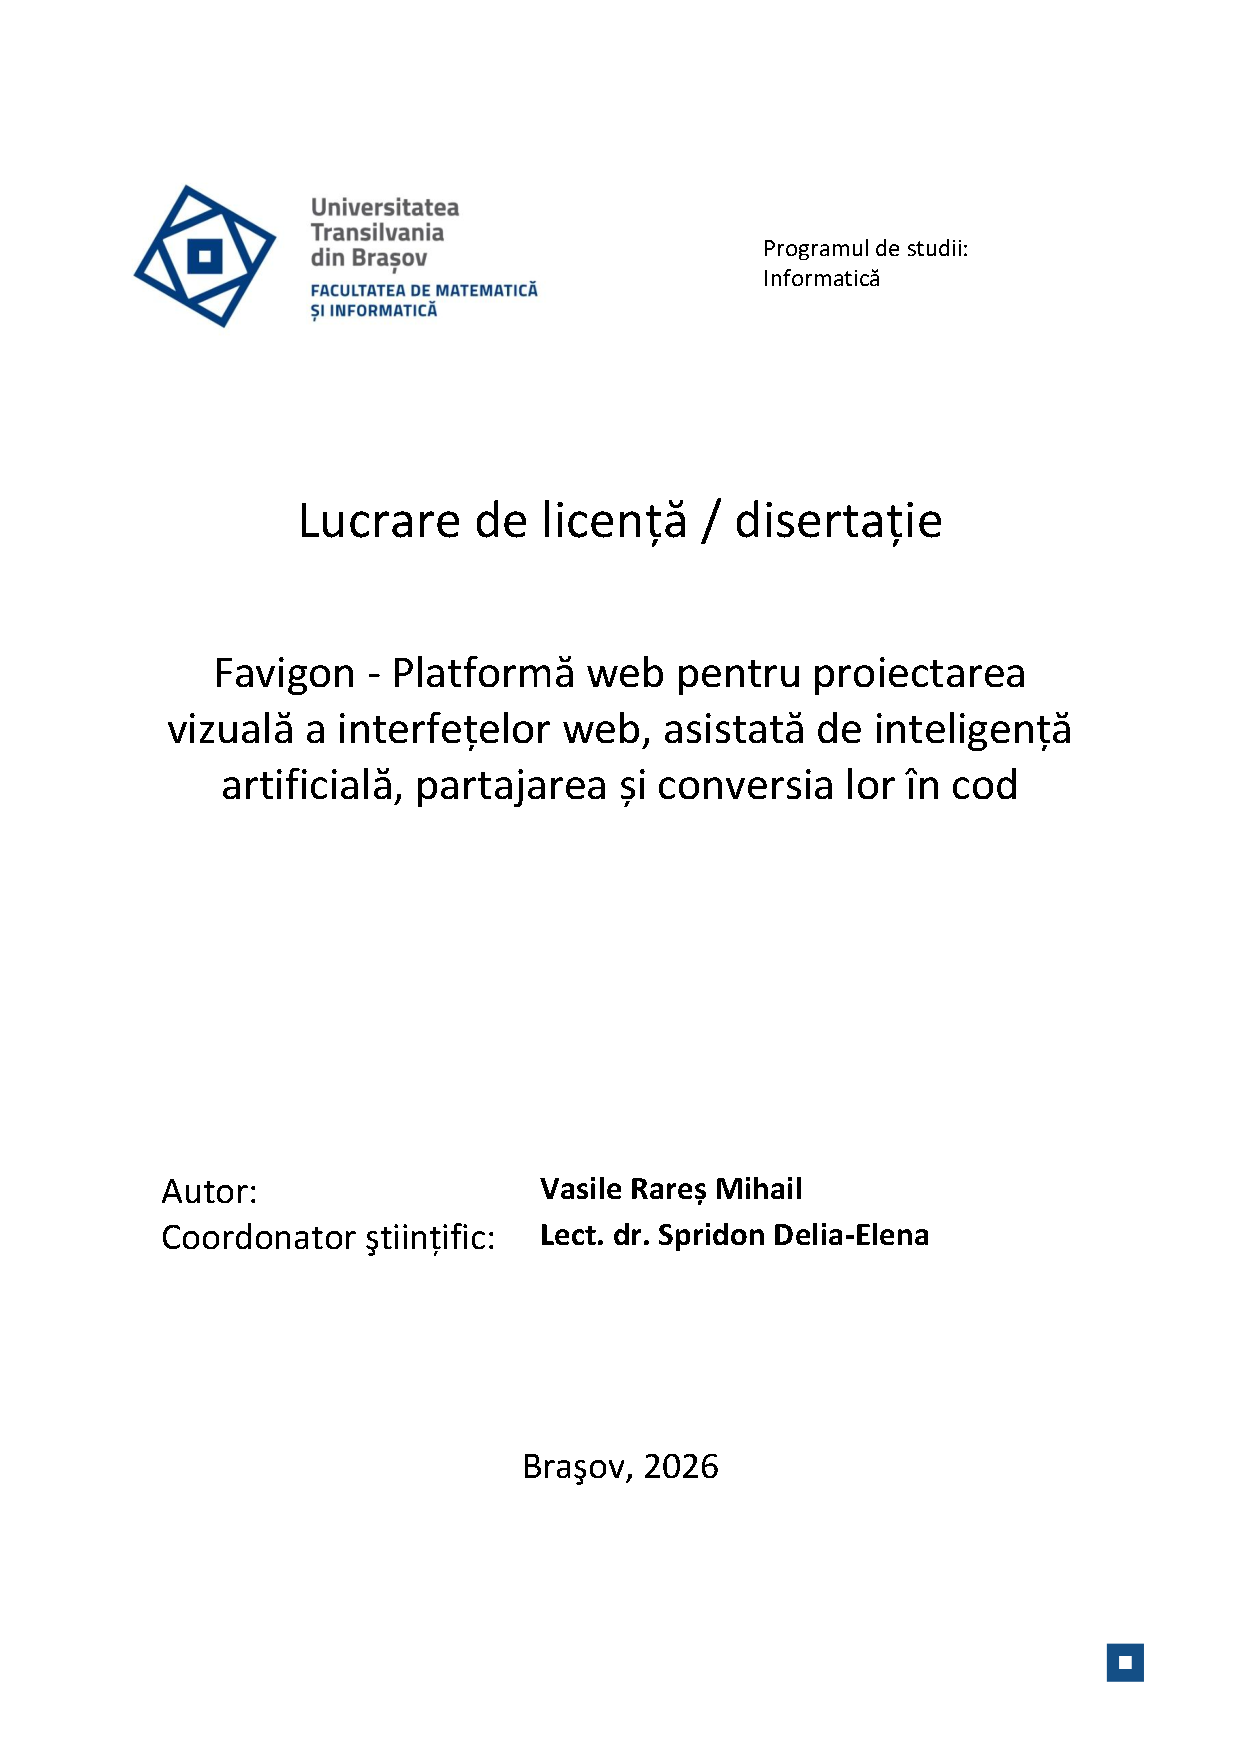
\includepdf[pages=1]{coperta licenta MI.pdf}

\pagenumbering{roman}

\chapter*{Rezumat}
\addcontentsline{toc}{chapter}{Rezumat}
Lucrarea prezintă proiectarea și implementarea platformei \textit{Favigon}, o aplicație web full-stack orientată spre construirea, editarea, partajarea și exportul interfețelor web. Ideea proiectului a pornit de la o observație simplă: în multe fluxuri de lucru actuale, trecerea de la design la cod rămâne fragmentată. Designerul lucrează într-un instrument, dezvoltatorul reconstruiește manual interfața, iar utilizatorul final vede rezultatul abia după mai multe iterații. În cazul proiectelor mici această separare este suportabilă, însă pentru proiecte dinamice devine rapid o sursă de timp pierdut, nealiniere și compromisuri tehnice.

În acest context, lucrarea urmărește realizarea unei platforme care să combine mai multe direcții într-un singur produs: editare vizuală într-un canvas, generare asistată de inteligență artificială, export de cod pentru mai multe framework-uri și o zonă socială în care proiectele pot fi publicate, apreciate și reutilizate. În forma actuală, Favigon se adresează în special designerilor, frontend developerilor, studenților și echipelor mici care vor să transforme rapid o idee de interfață într-un prototip editabil, într-un model intern coerent și, la final, în cod executabil. Din punct de vedere tehnic, aplicația folosește un frontend dezvoltat în Angular 20, un backend REST realizat în ASP.NET Core 9, o bază de date PostgreSQL și o infrastructură containerizată cu Docker Compose. Pentru expunerea aplicației în exterior este folosit și un tunel Cloudflare.

O parte importantă a lucrării este reprezentată de editorul canvas. Acesta nu este tratat ca o simplă interfață de desen, ci ca un subsistem complex, cu stare proprie, istoric de editare, persistare automată, operații de clipboard, gesturi de manipulare și suport pentru mai multe pagini. În jurul lui este construit un model de date orientat pe elemente și pagini, iar pe frontend logica este organizată în servicii dedicate pentru viewport, gesturi, istoric, persistare și generare de cod. Această separare menține codul relativ ușor de extins și evită concentrarea tuturor responsabilităților într-o singură componentă.

Capitolul central al lucrării este dedicat funcționalității de generare asistată de AI și conversiei din design în cod. În locul unei generări directe, greu de controlat, este folosită o soluție în trei faze. Prima fază extrage intenția utilizatorului și definește structura logică a paginii. A doua fază generează o reprezentare intermediară a interfeței, bazată pe un arbore de noduri cu informații de layout, stil, poziționare și metadate. A treia fază aplică stilizarea finală, păstrând structura deja validată. În acest mod, partea de AI poate fi constrânsă mai bine, iar rezultatele sunt mai ușor de verificat și reparat atunci când modelul produce ieșiri imperfecte.

Conversia în cod folosește aceeași reprezentare intermediară și o transformă în fișiere pentru HTML, React și Angular. Astfel, editorul și motorul de export nu sunt legate rigid de un singur framework. Din punct de vedere practic, această decizie a fost una dintre cele mai importante din proiect, deoarece a separat clar problema construirii designului de problema randării lui într-o tehnologie concretă. În plus, platforma suportă și export multi-page, precum și generare responsive prin diferențe între breakpoints.

Lucrarea tratează și componentele conexe care fac aplicația utilizabilă ca produs, nu doar ca demo tehnic: autentificare cu JWT în cookie-uri, OAuth prin furnizori externi, resetare parolă, autentificare în doi pași, gestiunea profilului, proiecte publice și private, explorare de proiecte și funcții sociale precum like, star, follow sau fork. În plus, sunt prezentate măsurile de securitate aplicate în backend, cum ar fi rate limiting-ul, limitarea dimensiunii cererilor, middleware-ul de tratare a excepțiilor și politicile de securitate HTTP.

Pentru validare, proiectul include atât testare automată, cât și scenarii funcționale. La momentul redactării lucrării, suita de teste backend conține 108 teste care verifică servicii, controllere, middleware și motorul de conversie. Partea de frontend este testată mai puțin automatizat, motiv pentru care în lucrare sunt prezentate și validarea prin scenarii operaționale, observații directe și demonstrarea fluxurilor principale.

Rezultatul final este o platformă care nu încearcă să înlocuiască instrumentele consacrate din ecosistem, ci să ofere un flux integrat pentru proiectare rapidă, experimentare, export și publicare. Aportul personal se reflectă mai ales în integrarea coerentă a acestor module, în modelul intermediar folosit pentru design și cod, în pipeline-ul AI în trei faze și în modul în care editorul canvas a fost separat pe servicii specializate. În ansamblu, proiectul a permis combinarea unor teme de arhitectură software, dezvoltare web, securitate, UX și inteligență artificială aplicată într-un produs unitar.


\tableofcontents
\listoffigures
\listoftables

\clearpage
\pagenumbering{arabic}

\chapter{Introducere}

\section{Contextul actual al temei}

În ultimii ani, dezvoltarea produselor digitale a devenit tot mai dependentă de colaborarea dintre roluri diferite: designeri, frontend developeri, backend developeri, product manageri și, din ce în ce mai des, sisteme automate bazate pe inteligență artificială. Dincolo de faptul că aceste roluri folosesc instrumente diferite, ele gândesc produsul și la niveluri de abstractizare diferite. Designerul lucrează cu layout, ierarhie vizuală și consistență. Dezvoltatorul web lucrează cu componente, stare, apeluri HTTP, validări și performanță. În practică, diferența dintre aceste două perspective produce aproape mereu un cost suplimentar în procesul de implementare.

Într-o aplicație web clasică de tip SPA, interfața nu mai este doar o succesiune de pagini statice. Ea este rezultatul unor stări multiple, a rutării client-side și a interacțiunilor asincrone cu serverul, ceea ce face ca proiectarea și implementarea să fie strâns legate \cite{fielding2000rest,angularRouting2026}. În același timp, ecosistemul modern a produs o gamă largă de instrumente specializate: unele pun accent pe design și handoff, altele pe no-code, altele pe generare de cod sau pe conținut. Deși fiecare rezolvă o parte a problemei, fluxul complet rămâne adesea fragmentat.

Aplicații precum Figma, Webflow, Framer sau Builder.io ilustrează foarte bine această tendință. Figma oferă un mediu matur pentru design și inspecție tehnică, cu suport pentru Dev Mode și conectare la cod \cite{figmaDevMode2026}. Webflow mută accentul spre construcția vizuală a site-urilor și publicarea rapidă \cite{webflow2026}. Framer împinge zona de prototipare și generare de layout cu ajutorul AI \cite{framerWireframer2026}. Builder.io propune un model de dezvoltare vizuală cu integrare în cod și AI orientat spre reutilizarea componentelor existente \cite{builderPlatform2026,builderAi2026}. Tocmai această diversitate arată că problema nu este încă închisă și că există loc pentru experimente și soluții integrate.

\section{Problema pe care o urmărește lucrarea}

Problema de la care pornește lucrarea este una concretă: cum poate fi redusă distanța dintre ideea de interfață, reprezentarea ei vizuală și codul care ajunge efectiv să ruleze într-un browser? În fluxul obișnuit, utilizatorul descrie o nevoie, designerul desenează o soluție, dezvoltatorul o reconstruiește în cod, iar echipa verifică manual dacă rezultatul este apropiat de intenția inițială. Fiecare transfer dintre etape introduce timp de așteptare, ambiguitate și posibile erori.

Din această observație rezultă trei subprobleme. Prima este problema editării vizuale: utilizatorul are nevoie de un spațiu în care să poată construi o pagină, să repoziționeze elemente, să lucreze cu mai multe pagini și să își poată salva progresul fără operații tehnice inutile. A doua este problema structurării interfeței: dacă se dorește folosirea AI sau exportul de cod, nu este suficientă existența unei imagini convingătoare, ci este necesară o reprezentare internă coerentă, stabilă și validabilă. A treia este problema reutilizării: odată ce un design există, el ar trebui să poată fi publicat, apreciat, partajat și eventual preluat de alți utilizatori.

În multe produse existente aceste trei subprobleme sunt tratate separat. Există editoare vizuale foarte bune, dar fără export tehnic serios. Există generatoare AI interesante, dar greu de controlat. Există convertoare către cod, dar care pornesc de la intrări rigide și nu oferă un spațiu de lucru propriu-zis. În cadrul acestui proiect, ele sunt tratate împreună, într-o platformă unitară.

Formulat direct, ideea proiectului este următoarea: Favigon este o platformă web pentru designeri, frontend developeri, studenți și echipe mici care doresc să reducă distanța dintre concept, prototip editabil și cod executabil. Accentul nu cade pe publicarea imediată a unui site, ci pe construirea unui flux coerent în care interfața poate fi desenată, structurată, validată, exportată și apoi reutilizată.

\section{Motivația alegerii temei}

Tema a fost aleasă deoarece reunește mai multe direcții relevante pentru un proiect de licență. În primul rând, are o componentă clară de arhitectură software. Un produs de tipul Favigon nu poate fi realizat doar ca interfață sau doar ca API, deoarece valoarea lui apare tocmai din cooperarea mai multor subsisteme. Din acest motiv, tema a impus decizii reale de separare a responsabilităților, persistare, modelare a datelor și organizare a codului.

În al doilea rând, tema are o componentă puternică de experiență a utilizatorului. Editorul canvas nu este util dacă doar ``funcționează'' tehnic. El trebuie să fie suficient de fluid încât utilizatorul să simtă că poate experimenta fără fricțiune mare. Asta înseamnă zoom, selecție, pan, istoric, clipboard, editare text, previzualizare și salvare automată. Practic, multe decizii de implementare au fost influențate direct de comportamentul așteptat în interfață.

În al treilea rând, integrarea AI într-un produs real reprezintă un subiect actual și util, dar numai dacă este tratată pragmatic. Interesul nu este folosirea inteligenței artificiale ca element decorativ, ci ca mecanism care poate accelera generarea unei structuri inițiale și poate reduce timpul dintre idee și rezultat. De aceea este evitată o soluție bazată doar pe prompt și este introdus un pipeline etapizat, cu validare și constrângeri explicite prin JSON Schema \cite{jsonSchemaCore2022,jsonSchemaValidation2022,openaiStructuredOutputs2026}.

\section{Obiectivele proiectului}

Obiectivul general al proiectului este proiectarea și implementarea unei platforme web care să permită:

\begin{itemize}[leftmargin=1.5cm]
  \item crearea și editarea vizuală a interfețelor web într-un canvas;
  \item generarea asistată de AI a unei structuri inițiale pentru pagini;
  \item conversia interfețelor construite într-o reprezentare intermediară coerentă;
  \item exportul automat al rezultatului în HTML, React și Angular;
  \item publicarea și reutilizarea proiectelor într-un spațiu cu funcții sociale.
\end{itemize}

Pentru a atinge acest obiectiv general, au fost urmărite și o serie de obiective specifice:

\begin{enumerate}[leftmargin=1.5cm]
  \item proiectarea unei arhitecturi full-stack suficient de clare încât logica de business, persistența și integrarea externă să nu fie amestecate;
  \item definirea unui model de date care să acopere utilizatorii, proiectele, relațiile sociale și legăturile externe de autentificare;
  \item dezvoltarea unui editor canvas care să poată gestiona mai multe pagini și mai multe tipuri de operații de editare;
  \item introducerea unei reprezentări intermediare reutilizabile atât de editor, cât și de motorul de conversie;
  \item dezvoltarea unui pipeline AI în mai multe faze, pentru a crește controlul asupra ieșirii;
  \item validarea soluției atât prin testare automată, cât și prin scenarii funcționale.
\end{enumerate}

Pe parcursul implementării, a fost păstrată o regulă simplă: fiecare funcționalitate nouă trebuie să aducă valoare clară în produs și să poată fi justificată tehnic. Din acest motiv, anumite idei care ar fi mărit spectaculos aplicația, dar fără un câștig real de coerență, au fost lăsate pentru dezvoltări viitoare.

\section{Contribuțiile proprii}

Aportul personal din această lucrare se vede în principal în șase direcții.

Prima direcție este integrarea într-un produs unitar a unor funcții care, de regulă, apar în produse diferite: editor vizual, generare AI, conversie în cod și distribuire socială. Miza nu a fost doar adăugarea mai multor module, ci și funcționarea lor pe aceeași bază de date, pe aceeași logică de autentificare și pe același model intern.

A doua direcție este organizarea editorului canvas. În locul unei implementări monolitice, logica este separată pe servicii focalizate pentru viewport, istoric, clipboard, persistare, gesturi și randare. Această decizie nu este vizibilă imediat la nivel de interfață, dar a contat mult pentru stabilitatea dezvoltării ulterioare.

A treia direcție este reprezentarea intermediară a interfeței. Editorul nu lucrează doar cu elemente vizuale izolate, iar exportul nu pornește direct de la DOM. Între aceste niveluri există un model intern bazat pe noduri, layout, stil și poziționare, care face posibilă atât validarea, cât și exportul în mai multe tehnologii.

A patra direcție este pipeline-ul AI în trei faze: intenție, structură și stil. Această separare este utilă deoarece generarea directă a codului sau a designului final este mai greu de controlat. În schimb, dacă problema este spartă în pași mai mici, fiecare pas poate fi verificat mai ușor și, la nevoie, reparat.

A cincea direcție este motorul de conversie. Acesta nu generează doar un singur rezultat static, ci suportă export single-page, multi-page și responsive. În plus, aceeași bază este folosită pentru HTML, React și Angular, ceea ce obligă la o abstracție mai curată decât în cazul unui export dedicat unei singure ținte.

A șasea direcție este componenta de produs: autentificare cu 2FA, OAuth, proiecte publice și private, explore, like, star, follow și fork. Aceste funcții schimbă proiectul dintr-un simplu editor tehnic într-o platformă care poate susține colaborare și reutilizare.

\section{Metoda de lucru}

Din punct de vedere practic, dezvoltarea aplicației a fost iterativă. Procesul a început cu funcționalitățile de bază necesare pentru existența produsului: autentificare, proiecte și editor minimal. După aceea, au fost adăugate treptat comportamente mai complexe în editor, persistare automată și suport pentru export. Abia după ce această bază a devenit suficient de stabilă a fost integrat pipeline-ul AI, deoarece fără un model intern coerent rezultatele generate ar fi fost greu de controlat.

Pe partea de backend a fost urmărită o structură apropiată de principiile prezentate în literatura de arhitectură software \cite{bass2021softwarearchitecture,martin2017cleanarchitecture}. Asta a însemnat separarea API-ului de logica de aplicație, a logicii de aplicație de infrastructură și folosirea interfețelor între straturi. Nu a fost urmărită o implementare dogmatică, ci una practică: suficient de clară ca să poată susține extinderea proiectului, dar fără un volum de abstracții inutile.

Pe partea de frontend, strategia a fost păstrarea logicii specifice editorului în interiorul feature-ului canvas, nu într-o zonă generică de utilitare sau componente partajate. Din moment ce editorul concentrează cea mai mare parte din complexitatea aplicației, această decizie a ajutat la evitarea dispersării comportamentelor și la păstrarea contextului tehnic aproape de ecranele care îl folosesc.

\section{Structura lucrării}

Lucrarea este organizată în opt capitole principale și trei anexe.

Capitolul al doilea analizează domeniul și compară Favigon cu aplicații existente. Capitolul al treilea prezintă fundamentele teoretice și tehnologiile folosite. Capitolul al patrulea tratează analiza cerințelor și proiectarea sistemului. Capitolul al cincilea descrie implementarea platformei la nivel de module și fluxuri principale. Capitolul al șaselea este dedicat generării asistate de AI și conversiei din design în cod, acesta fiind și nucleul tehnic al lucrării. Capitolul al șaptelea abordează securitatea, testarea și validarea. Ultimul capitol sintetizează concluziile și direcțiile de dezvoltare.

Anexele completează partea principală cu scenarii demo, note de arhitectură și o vedere de ansamblu asupra API-ului. Această structură separă mai clar fundamentarea teoretică de implementarea efectivă și păstrează contribuțiile personale vizibile în partea centrală a lucrării, nu ascunse între noțiuni generale.

\chapter{Analiza domeniului și studiu comparativ}

\section{Evoluția spațiului design-to-code}

Zona de \textit{design-to-code} nu este nouă, dar a devenit mult mai vizibilă odată cu maturizarea aplicațiilor web și cu apariția modelelor generative moderne. În literatura mai veche, problema era formulată deseori ca transformarea unei descrieri vizuale într-un cod de interfață. Un exemplu cunoscut este \textit{pix2code}, unde autorul tratează generarea codului din capturi de ecran ale interfeței \cite{beltramelli2017pix2code}. Mai recent, lucrările dedicate modelelor mari de limbaj și modelelor multimodale arată că interesul s-a mutat de la simpla reconstrucție a aspectului spre păstrarea structurii, a layout-ului și a intenției de produs \cite{shen2024uicoder,xu2025latcoder}.

În practică, piața a evoluat într-o direcție puțin diferită de lucrările academice. Produsele comerciale au observat că utilizatorul nu are nevoie doar de un model care produce cod, ci de un întreg flux de lucru: proiectare, organizare pe pagini, colaborare, verificare, export, publicare și iterație. Din acest motiv, instrumentele moderne nu mai pot fi analizate doar prin întrebarea ``generează sau nu cod?'', ci prin ansamblul de funcții pe care îl oferă.

Mai există și un detaliu important. În multe situații, problema nu este că nu se poate genera ceva, ci că rezultatul generat nu este suficient de ușor de integrat într-un produs real. Un layout poate arăta bine ca demonstrație, dar dacă nu are o structură logică, dacă nu respectă constrângeri tehnice și dacă nu poate fi controlat prin iterații mici, valoarea lui practică scade. Această observație a influențat direct proiectarea Favigon: în loc să trateze AI-ul ca pe un generator final, platforma îl include într-un lanț controlat, în care reprezentarea intermediară și validarea joacă un rol central.

\section{Criterii de comparație}

Pentru a poziționa corect proiectul, au fost alese criterii relevante atât din punct de vedere tehnic, cât și din punct de vedere al utilității pentru utilizator:

\begin{itemize}[leftmargin=1.5cm]
  \item \textbf{editare vizuală directă}: existența unui spațiu de lucru de tip canvas sau editor vizual;
  \item \textbf{asistență AI}: posibilitatea de a porni de la un prompt, sugestii sau generare automată de structură;
  \item \textbf{design-to-code}: existența unei conversii către cod sau măcar a unor artefacte pentru handoff tehnic;
  \item \textbf{orientare spre produs final}: suport pentru publicare, organizare pe pagini sau dezvoltare continuă;
  \item \textbf{partajare și colaborare}: mecanisme prin care rezultatele pot fi distribuite sau reutilizate;
  \item \textbf{control tehnic al ieșirii}: cât de mult poate fi influențată structura rezultatului și cât de ușor poate fi integrat în cod existent.
\end{itemize}

Aceste criterii nu sunt perfecte și nu încearcă să stabilească ``cel mai bun'' produs. Scopul lor este mai modest: să arate unde se află Favigon pe o hartă a instrumentelor existente și ce gol încearcă să acopere.

\section{Aplicații relevante din aceeași zonă}

\subsection{Figma}

Figma este, în mod firesc, un punct de referință pentru orice discuție despre proiectarea interfețelor. Din perspectiva acestei lucrări, interesul nu este dat doar de partea de design colaborativ, ci și de Dev Mode. Documentația oficială arată clar că Dev Mode este gândit ca spațiu pentru inspectarea designurilor și pentru apropierea dintre design și implementare \cite{figmaDevMode2026}. Cu toate acestea, Figma rămâne în primul rând un instrument de design și handoff. Chiar dacă poate genera fragmente de cod sau poate conecta design system-uri la bazele de cod, el nu devine automat un mediu complet de construire și publicare a produsului.

Pentru Favigon, Figma este util mai ales ca termen de comparație în două direcții. Prima direcție este ideea de structură vizuală clară și multi-page. A doua este faptul că handoff-ul către dezvoltare nu este suficient în sine; dacă se urmăresc iterații rapide, este necesar un spațiu în care designul să poată fi nu doar inspectat, ci și transformat mai departe în ceva executabil.

\subsection{Webflow}

Webflow este relevant deoarece reprezintă foarte bine zona de \textit{visual website builder}. Pagina oficială pune accent pe construcția vizuală, publicare și generare rapidă de site-uri \cite{webflow2026}. Avantajul evident al acestei abordări este că rezultatul ajunge repede online și este ușor de gestionat din punct de vedere al conținutului. În schimb, Webflow are un focus clar pe zona de website publishing și CMS, nu pe un model general de interfață reutilizabil între mai multe framework-uri.

Pentru poziționarea Favigon, Webflow este important tocmai pentru a delimita intenția aplicației. Nu a fost urmărită construirea încă unui publicator vizual de site-uri. Accentul cade mai mult pe controlul tehnic al structurii, exportul în cod și legătura dintre un editor vizual și o reprezentare internă care poate fi convertită.

\subsection{Framer}

Framer este interesant fiindcă mută discuția mai aproape de zona AI. Pagina oficială pentru Wireframer arată o abordare în care un prompt este folosit pentru a construi rapid un layout responsive, cu accent pe structură și flux \cite{framerWireframer2026}. Este o direcție apropiată de cea urmărită și aici, însă diferența majoră este că în Favigon este făcută explicită separarea dintre intenție, structură și stilizare.

Cu alte cuvinte, Framer demonstrează că generarea ghidată de prompt poate fi utilă pentru pornirea rapidă a unui proiect. Totuși, pentru o lucrare inginerească este mai valoros să fie explicați și controlați pașii interni ai generării, nu doar să fie observat rezultatul final.

\subsection{Builder.io}

Builder.io este probabil cel mai apropiat reper comercial pentru direcția urmărită în această lucrare. Platforma lor pune accent pe dezvoltare vizuală, AI și reutilizarea componentelor existente \cite{builderPlatform2026,builderAi2026}. Ideea de a nu porni de la zero de fiecare dată, ci de a avea o punte între design, componente și cod, este una foarte relevantă.

Diferența principală este că Builder.io este orientat puternic spre integrarea într-un ecosistem existent și spre productivitate în contexte enterprise. Favigon, în schimb, este un proiect academic și experimental, în care accentul este pus pe claritatea modelului intern și pe trasabilitatea tehnică a fiecărei etape. Asta înseamnă că produsul nu concurează direct cu Builder.io la nivel de maturitate comercială, dar tratează o parte din probleme într-un mod mai transparent pentru analiză și explicație.

\section{Tabel comparativ}

\begin{table}[H]
  \centering
  \caption{Comparație între Favigon și aplicații relevante}
  \label{tab:comparatie-platforme}
  \renewcommand{\arraystretch}{1.2}
  \begin{tabularx}{\textwidth}{>{\RaggedRight\arraybackslash}p{3.1cm}YYYYY}
    \toprule
    \textbf{Criteriu} & \textbf{Figma} & \textbf{Webflow} & \textbf{Framer} & \textbf{Builder.io} & \textbf{Favigon} \\
    \midrule
    Editor vizual direct & Da & Da & Da & Da & Da \\
    Pornire din prompt AI & Parțial & Da & Da & Da & Da \\
    Model intern orientat spre export multi-framework & Nu explicit & Nu & Limitat & Parțial & Da \\
    Export către HTML/React/Angular & Nu ca obiectiv principal & Nu în forma urmărită aici & Limitat & Orientat pe integrare & Da \\
    Funcții sociale în aceeași platformă & Nu & Nu & Nu & Nu & Da \\
    Publicare proiecte proprii & Parțial & Da & Da & Da & Parțial \\
    Reutilizare prin fork / star / like & Nu & Nu & Nu & Nu & Da \\
    Accent pe controlul etapelor AI & Nu & Nu & Parțial & Parțial & Da \\
    \bottomrule
  \end{tabularx}
\end{table}

Tabelul~\ref{tab:comparatie-platforme} nu are rolul de a demonstra că Favigon este ``mai bun'' decât produsele consacrate. Ar fi o comparație nerealistă. Scopul lui este să arate că Favigon combină, într-o formă academică și experimentală, elemente care în alte produse apar separate: editor vizual, asistență AI, export în cod și funcții sociale.

\section{Poziționarea proiectului Favigon}

În urma comparației, Favigon poate fi poziționat ca o platformă experimentală de tip \textit{AI-assisted visual builder}, orientată mai puțin spre publicare imediată și mai mult spre explorarea unui flux coerent între idee, design, model intern și cod executabil. Cu alte cuvinte, produsul nu își propune să concureze prin maturitatea ecosistemului, ci prin claritatea traseului tehnic pe care îl oferă.

În termeni practici, produsul este mai potrivit pentru prototipare rapidă, experimente de interfață, proiecte academice și aplicații mici sau medii decât pentru scenarii enterprise foarte rigide. Această delimitare este importantă, deoarece explică mai bine valoarea reală a platformei: nu promite înlocuirea unui ecosistem comercial matur, ci oferă un cadru integrat pentru a trece mai repede de la idee la un rezultat executabil și analizabil tehnic.

Această poziționare vine și cu limite. De exemplu, Favigon nu are nivelul de rafinament vizual sau de integrare enterprise al unor produse comerciale mature. Nici partea de colaborare simultană în timp real nu este încă implementată. Totuși, pentru scopul lucrării, aceste limite nu sunt un dezavantaj major. Ele permit concentrarea pe întrebările urmărite aici:

\begin{itemize}[leftmargin=1.5cm]
  \item cum pot reprezenta o interfață într-o formă suficient de stabilă încât să o editez și să o export;
  \item cum pot integra AI într-un mod controlabil;
  \item cum pot susține reutilizarea prin funcții sociale simple;
  \item cum pot organiza întregul produs astfel încât să rămână clar tehnic.
\end{itemize}

\section{Golul pe care îl acoperă Favigon}

Din analiza de mai sus rezultă că există un spațiu intermediar între instrumentele clasice de design, generatoarele AI rapide și platformele orientate strict spre publicare. Favigon încearcă să acopere tocmai acest spațiu intermediar. Mai exact, platforma propune:

\begin{enumerate}[leftmargin=1.5cm]
  \item un editor propriu, nu doar o zonă de import sau inspectare;
  \item un model intermediar explicit, nu doar un rezultat final opac;
  \item export multi-framework, nu doar un cod specific unei singure ținte;
  \item funcții sociale integrate, astfel încât proiectele să poată circula în comunitate;
  \item o integrare a AI-ului care poate fi analizată, validată și îmbunătățită pas cu pas.
\end{enumerate}

Din punct de vedere academic, acesta reprezintă un unghi bun pentru o lucrare de licență. Proiectul nu se reduce la folosirea unui model AI pentru obținerea unor pagini, ci pune în discuție mai multe aspecte inginerești: modelare internă, arhitectură pe straturi, validare, testare, UX și decizii de produs.

\section{Concluzii intermediare}

Analiza domeniului arată că proiectul Favigon nu apare într-un vid, ci într-un context în care instrumentele pentru design, dezvoltare vizuală și AI cresc rapid. În același timp, ea arată și de ce proiectul are sens ca temă de licență. Există deja instrumente puternice, dar nu toate tratează împreună editarea vizuală, generarea controlată, exportul tehnic și partajarea în aceeași platformă.

Concluzia acestui capitol este că Favigon nu trebuie evaluat ca un produs comercial finalizat, ci ca o platformă software care încearcă să demonstreze fezabilitatea unui flux integrat. Pe baza acestei concluzii, capitolul următor trece de la piață și comparații la fundamentele teoretice și tehnologiile pe care s-a sprijinit implementarea.

\chapter{Fundamente teoretice și tehnologii utilizate}

\section{Considerații generale}

Înainte de a descrie implementarea concretă, este utilă clarificarea fundamentelor pe care se sprijină proiectul. Favigon nu reunește doar câteva ecrane și endpoint-uri, ci mai multe idei care trebuie să funcționeze împreună: aplicație single-page, API REST, autentificare pe bază de token, persistare relațională, orchestrare containerizată, generare asistată cu ieșiri structurate și conversie dintr-un model intermediar către cod executabil.

Aceste noțiuni sunt tratate împreună deoarece în proiect ele nu apar izolat. De exemplu, editorul canvas este implementat pe frontend, dar depinde direct de modul în care proiectele sunt persistate în backend. Pipeline-ul AI produce o structură intermediară, dar valoarea ei reală se vede abia când motorul de conversie o transformă în fișiere HTML, React sau Angular. Din acest motiv, capitolul de față urmărește să explice nu doar \textit{ce} tehnologii sunt folosite, ci și \textit{de ce} alegerea lor a fost potrivită pentru problema rezolvată.

\section{Aplicații single-page și rolul frontend-ului modern}

Favigon folosește pe partea de client o aplicație Angular 20 organizată sub forma unui SPA. Într-un SPA, browserul încarcă inițial o singură pagină, iar apoi navigarea între ecrane este gestionată în principal client-side, fără reîncărcarea completă a documentului \cite{angularRouting2026}. Acest model este potrivit pentru Favigon din două motive.

Primul motiv este experiența utilizatorului. Editorul canvas presupune interacțiuni dese, actualizări vizuale rapide și trecere fluidă între zone precum profil, explore, settings, proiect și preview. Dacă fiecare navigare ar depinde de reîncărcarea integrală a paginii, aplicația ar deveni mai greu de folosit și mai puțin apropiată de instrumentele moderne de design.

Al doilea motiv este organizarea tehnică. Angular oferă rutare, componente, injecție de dependențe, gestiune a formularelor și integrare cu HTTP într-un ecosistem unitar. În plus, proiectul folosește componente standalone și `provideRouter`, ceea ce simplifică structura aplicației și reduce dependența de module tradiționale \cite{angularProvideRouter2026,angularStandalone2026}. Pentru un proiect în care cea mai mare complexitate se află în interfață, această coerență a framework-ului a contat mult.

Un element important în implementare este folosirea \textit{signals}. Documentația Angular prezintă signals ca mecanism reactiv granular pentru urmărirea și actualizarea stării \cite{angularSignals2026}. În editorul canvas, această abordare este utilă deoarece permite reacții mai fine la schimbarea selecției, a viewport-ului, a paginii curente sau a istoricului, fără a introduce un strat extern de management al stării. Pentru un feature foarte interactiv, această soluție oferă un raport bun între simplitate și control.

\section{Arhitectura client-server și API-ul REST}

Comunicarea dintre frontend și backend este organizată sub forma unui API REST. În literatura clasică, stilul REST este tratat ca o modalitate de proiectare a sistemelor software bazate pe resurse, interacțiuni standardizate și separarea clară între client și server \cite{fielding2000rest}. În Favigon, această alegere a fost una pragmatică.

Aplicația are resurse destul de clar delimitate: utilizatori, proiecte, design-uri, upload-uri, rezultate generate, relații sociale și operații de autentificare. Pentru fiecare dintre acestea a fost naturală definirea unor controllere și endpoint-uri specializate. Spre exemplu, proiectele sunt gestionate prin endpoint-uri dedicate pentru creare, actualizare, design, thumbnail, assets, like, star sau fork, în timp ce autentificarea este separată în propriul controller.

ASP.NET Core 9 a fost ales pentru backend deoarece oferă un cadru potrivit pentru API-uri moderne: rutare declarativă, middleware configurabil, DI integrat, autentificare, autorizare și extensibilitate la nivel de pipeline HTTP. Dincolo de faptul că framework-ul este matur, el permite și o separare curată între straturile aplicației. În proiect, API-ul doar primește cereri și returnează răspunsuri, în timp ce logica de business este ținută în servicii de aplicație, iar persistența și integrarea externă sunt mutate în infrastructură.

\section{Autentificare, token-uri și securitate la nivel de cerere}

Zona de autentificare din Favigon combină mai multe mecanisme: login și register clasic, OAuth cu furnizori externi, refresh token și autentificare în doi pași. Din perspectiva acestei lucrări, important este modul în care ele sunt integrate coerent.

ASP.NET Core oferă suport direct pentru autentificare JWT bearer \cite{aspnetJwt2025}. În proiect, token-ul de acces este transportat prin cookie HTTP only, iar backend-ul îl extrage din cookie-ul `jwt` în cadrul configurării `JwtBearer`. Practic, acest lucru combină avantajul token-ului auto-conținut cu avantajul unui transport mai greu de accesat din JavaScript. Această alegere nu elimină orice risc posibil, dar este rezonabilă pentru tipul de aplicație construit aici.

În plus, proiectul folosește refresh token separat și limitează calea cookie-ului de refresh la endpoint-ul de reînnoire, ceea ce reduce suprafața de expunere. Pentru operații sensibile sau scenarii de risc mai mare, este introdusă și autentificare în doi pași pe bază de cod temporar transmis prin email. Din perspectiva ghidurilor OWASP, folosirea unui factor suplimentar este una dintre cele mai eficiente măsuri pentru reducerea atacurilor care pornesc de la compromiterea parolei \cite{owaspAuth2026,owaspMfa2026}.

Dincolo de autentificare, backend-ul folosește și rate limiting. Documentația ASP.NET Core tratează rate limiting-ul ca mecanism de control al fluxului de cereri, util pentru protecție împotriva abuzului și pentru stabilitate \cite{aspnetRateLimiting2025}. În proiect sunt definite politici diferite pentru zone precum autentificare, AI, converter și users, tocmai pentru că profilul de risc și costul operațiilor nu sunt aceleași.

\section{Reprezentarea intermediară a interfeței}

Una dintre ideile de bază ale proiectului este că designul nu trebuie legat direct nici de canvas, nici de HTML final. Între aceste două niveluri este introdusă o reprezentare intermediară bazată pe noduri (`IRNode`), layout, stil, poziționare, metadate și variante responsive. Din punct de vedere conceptual, această reprezentare joacă rolul unui limbaj intern al aplicației.

Avantajul principal al unui astfel de model este separarea preocupărilor. Editorul poate să manipuleze elemente și structuri fără să producă imediat cod pentru browser. În același timp, motorul de conversie poate genera HTML, React sau Angular fără să depindă de detaliile de implementare ale editorului. Asta înseamnă că aceeași structură poate fi folosită în două scopuri diferite: editare și export.

În plus, modelul intermediar permite validare înainte de generare. Dacă un arbore de noduri este incomplet, inconsistent sau imposibil de randat corect, problema poate fi detectată înainte de etapa de export. Acesta este un avantaj important față de abordările care merg direct din prompt în cod. În Favigon, această validare intermediară face posibilă combinarea AI-ului cu un flux tehnic controlabil.

\section{JSON Schema și ieșiri structurate pentru AI}

În momentul în care s-a decis folosirea unui model AI pentru generarea interfețelor, una dintre primele probleme a fost fiabilitatea formatului de ieșire. Un răspuns foarte bun ca limbaj natural nu este automat util pentru o aplicație software. Este nevoie de date structurate, de câmpuri verificabile și de o formă care să poată fi procesată programatic.

Pentru această nevoie, JSON Schema este un instrument foarte potrivit. Specificația definește un mod standardizat de a exprima structura, tipurile și restricțiile unui document JSON \cite{jsonSchemaCore2022,jsonSchemaValidation2022}. În Favigon, schema este folosită pentru a constrânge ieșirile modelului AI atunci când se generează atât blueprint-ul intenției, cât și arborele intermediar al interfeței.

Din perspectiva OpenAI API, această idee este compatibilă cu \textit{structured outputs}, adică solicitarea unui răspuns care respectă o anumită schemă \cite{openaiStructuredOutputs2026,openaiChatCompletions2026}. Totuși, faptul că formatul este corect nu garantează automat că și conținutul este potrivit. De aceea, în implementare nu s-a mers doar până la schema JSON, ci au fost adăugate și validări semantice, plus un mecanism de reparare atunci când modelul produce ieșiri invalide sau incomplete.

\section{Baza de date relațională și persistența}

Pentru persistență este folosit PostgreSQL, prin Entity Framework Core și providerul Npgsql \cite{postgresql16docs2026,npgsqlEfCore2026}. Alegerea unei baze de date relaționale a fost firească, deoarece datele principale au relații clare: un utilizator poate avea mai multe proiecte, proiectele pot avea aprecieri și bookmark-uri, utilizatorii se pot urmări între ei, iar un proiect poate fi fork-uit din alt proiect.

Pe lângă modelul relațional clasic, aplicația păstrează și un câmp de tip JSON serializat pentru designul proiectului. Aici există un compromis asumat. Pe de o parte, datele vizuale ale canvas-ului sunt prea flexibile pentru a fi modelate comod în tabele relaționale fine. Pe de altă parte, utilizatorii, relațiile sociale și metadatele proiectelor se potrivesc foarte bine într-un model relațional. În practică, combinația dintre tabele relaționale și document JSON pentru design s-a dovedit suficient de echilibrată pentru scopul proiectului.

În implementarea concretă, schema rezultată este compactă, dar suficient de expresivă pentru produsul construit. Baza de date conține tabelele \texttt{users}, \texttt{projects}, \texttt{linked\_accounts}, \texttt{user\_follows}, \texttt{project\_bookmarks} și \texttt{project\_likes}. Tabelele relaționale descriu identitatea utilizatorului, proiectele, relațiile sociale și interacțiunile dintre utilizatori și proiecte, iar câmpul \texttt{DesignJson} din \texttt{projects} păstrează documentul de canvas sub formă \texttt{jsonb}. Această alegere permite filtrare și agregare eficientă pentru metadate, fără a forța fragmentarea structurii vizuale în numeroase tabele auxiliare.

Schema fizică include și constrângeri relevante pentru consistență. Email-ul utilizatorului este unic, conturile OAuth au unicitate atât pe perechea `(Provider, ProviderUserId)`, cât și pe perechea `(UserId, Provider)`, iar tabelele de tip follow, bookmark și like folosesc chei compuse pentru a preveni dublurile. În plus, proiectele folosesc o autoreferință prin `ForkedFromProjectId`, ceea ce face posibilă trasabilitatea unui fork fără a duplica separat noțiunea de proiect-sursă. Contextul EF Core completează automat timestamp-urile `CreatedAt` și `UpdatedAt`, astfel încât persistența să rămână coerentă și la nivel operațional, nu doar la nivel de structură.

\section{Orchestrare și infrastructură}

La nivel de infrastructură, proiectul folosește Docker Compose pentru definirea și pornirea serviciilor principale: baza de date PostgreSQL, API-ul, frontend-ul și tunelul Cloudflare \cite{dockerCompose2026,dockerComposeFile2026}. Această variantă reduce efortul necesar pentru pornirea locală și descrie într-un singur fișier dependențele dintre servicii, volumele persistente și rețeaua internă.

Avantajul principal al acestui mod de lucru este repetabilitatea. Când toate componentele importante sunt definite declarativ, mediul devine mai ușor de refăcut, de demonstrat și de mutat între sisteme. Pentru o lucrare de licență, acest aspect nu este deloc minor, deoarece ușurează demo-ul și reduce riscul ca aplicația să funcționeze doar pe o singură configurație locală.

În configurația actuală, fișierul \texttt{docker-compose.yml} nu pornește doar containerele, ci exprimă și câteva decizii operaționale utile. Baza de date are \textit{healthcheck}, astfel încât API-ul să nu pornească înainte ca PostgreSQL să fie pregătit pentru conexiuni. API-ul montează separat volumul pentru upload-uri, ceea ce permite persistența imaginilor și thumbnail-urilor independent de ciclul containerului. Frontend-ul este construit cu argument explicit pentru fișierul de mediu de producție, iar tunelul Cloudflare este atașat peste aplicația deja pornită, nu folosit ca substitut pentru rețeaua internă.

\begin{table}[H]
  \centering
  \caption{Servicii și volume definite în orchestrarea locală a proiectului}
  \label{tab:docker-servicii}
  \renewcommand{\arraystretch}{1.15}
  \begin{tabularx}{\textwidth}{>{\RaggedRight\arraybackslash}p{2.8cm}YY}
    \toprule
    \textbf{Serviciu / volum} & \textbf{Rol principal} & \textbf{Observații utile} \\
    \midrule
    \texttt{db} & instanță PostgreSQL 16 pentru persistența relațională & folosește \textit{healthcheck} cu \texttt{pg\_isready} și volum persistent dedicat \\
    \texttt{api} & aplicația ASP.NET Core expusă intern pe portul 8080 & depinde de sănătatea bazei de date și montează directorul de upload-uri \\
    \texttt{frontend} & aplicația Angular compilată pentru mediu de producție & depinde de API și rulează în aceeași rețea internă \\
    \texttt{cloudflared} & publicare externă controlată prin Cloudflare Tunnel & folosește token extern și pornește doar după frontend \\
    postgres data & persistă datele PostgreSQL & evită pierderea datelor la recrearea containerelor \\
    uploads data & persistă fișierele încărcate și thumbnail-urile & separă conținutul generat de ciclul de build/deploy \\
    \bottomrule
  \end{tabularx}
\end{table}

Pentru expunerea aplicației în exterior este folosit și Cloudflare Tunnel. Documentația oficială subliniază faptul că tunelul funcționează prin conexiuni doar outbound dintre infrastructura locală și rețeaua Cloudflare, evitând expunerea directă a unui IP public și reducând suprafața de atac \cite{cloudflareTunnel2026}. În proiect, această alegere a fost utilă mai ales pentru publicare și testare externă, fără a complica prea mult configurarea rețelei. Vederea simplificată a stack-ului rezultat este redată în Figura~\ref{fig:stack-favigon}.

\begin{figure}[H]
  \centering
  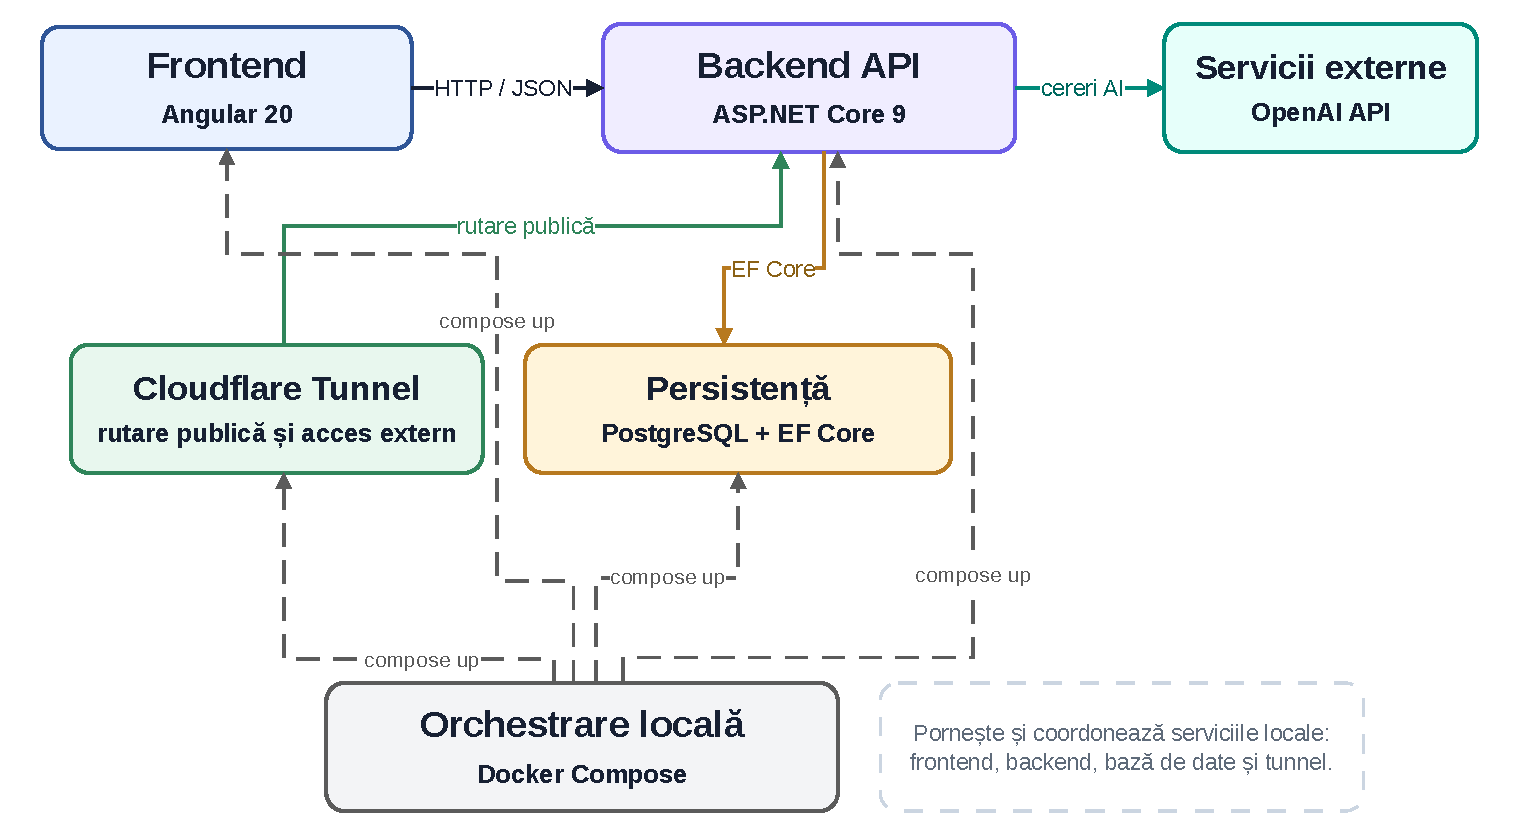
\includegraphics[width=\textwidth]{diagrams/stack-favigon.drawio.pdf}
  \caption{Vedere simplificată asupra stack-ului tehnologic folosit de Favigon}
  \label{fig:stack-favigon}
\end{figure}

\section{De ce această combinație tehnologică a fost potrivită}

Privită în ansamblu, combinația Angular + ASP.NET Core + PostgreSQL + OpenAI API + Docker Compose nu este una neobișnuită. Tocmai aici stă avantajul ei practic. Sunt folosite tehnologii bine documentate, mature și suficient de separate ca responsabilitate. Angular acoperă interfața și interacțiunea clientului. ASP.NET Core acoperă API-ul și middleware-ul. PostgreSQL acoperă persistența relațională. OpenAI API acoperă generarea asistată. Docker Compose și Cloudflare Tunnel simplifică operaționalizarea.

Această alegere are și un beneficiu pedagogic. Într-o lucrare de licență, prea multe tehnologii neobișnuite riscă să mute accentul de pe soluția inginerească pe complexitatea setării mediului. Aici valoarea nu vine din folosirea unor instrumente rare, ci din modul în care acestea sunt combinate pentru a obține un produs coerent.

\section{Concluzii intermediare}

Fundamentele prezentate în acest capitol explică de ce Favigon a fost construit în forma actuală. SPA-ul susține interacțiunea rapidă. API-ul REST și separarea pe straturi susțin claritatea backend-ului. JWT-ul, 2FA și rate limiting-ul susțin securitatea operațională. Reprezentarea intermediară și JSON Schema susțin controlul asupra generării AI și a exportului. PostgreSQL și Docker Compose susțin stabilitatea și portabilitatea.

Pe baza acestor fundamente, capitolul următor trece la analiza și proiectarea sistemului propriu-zis: cerințe, actori, fluxuri, model de date și arhitectură internă.



\chapter{Analiza și proiectarea sistemului}

\section{Pornirea de la cerințe}

Înaintea implementării funcționalităților principale, a fost necesară separarea cât mai clară a cerințelor sistemului. Pentru acest tip de proiect, riscul cel mai mare este adăugarea multor funcții atractive, dar fără o structură clară. De aceea, analiza a pornit de la întrebarea simplă: ce trebuie să poată face utilizatorul și ce trebuie să poată susține sistemul în spate?

Din perspectiva utilizatorului final, aplicația trebuie să permită crearea unui cont, autentificarea, administrarea profilului, lucrul cu proiecte și folosirea editorului vizual. Din perspectiva fluxului de produs, trebuie să existe și operații precum publicarea unui proiect, explorarea proiectelor altora, aprecierea lor și reutilizarea prin fork. Din perspectiva obiectivului tehnic al lucrării, sistemul trebuie să poată genera designuri cu ajutorul AI și să exporte rezultatul în cod.

Aceste cerințe au fost apoi grupate în două categorii mari: funcționale și nefuncționale.

\section{Cerințe funcționale}

Principalele cerințe funcționale identificate pentru Favigon sunt următoarele:

\begin{enumerate}[leftmargin=1.5cm]
  \item utilizatorul poate crea cont, autentifica și ieși din aplicație;
  \item utilizatorul poate folosi login clasic sau autentificare prin furnizori externi;
  \item utilizatorul poate activa sau dezactiva autentificarea în doi pași;
  \item utilizatorul își poate edita profilul și imaginea de profil;
  \item utilizatorul poate crea, edita și șterge proiecte;
  \item pentru fiecare proiect, utilizatorul poate salva designul și thumbnail-ul asociat;
  \item utilizatorul poate edita vizual proiectul într-un canvas cu mai multe pagini;
  \item utilizatorul poate genera o structură de design prin AI, inclusiv în regim streaming;
  \item utilizatorul poate valida și exporta proiectul în HTML, React sau Angular;
  \item utilizatorul poate marca proiectele altora cu like sau star;
  \item utilizatorul poate urmări alți utilizatori și poate vedea proiecte recomandate;
  \item utilizatorul poate fork-ui proiecte publice și le poate adapta în propriul spațiu.
\end{enumerate}

La nivel de implementare, aceste cerințe se reflectă destul de direct în controllerele și serviciile backend, respectiv în feature-urile frontend. De exemplu, `AccountController` și `AuthService` acoperă fluxurile de autentificare, `ProjectsController` și `ProjectService` gestionează ciclul de viață al proiectelor, iar `AiDesignController` împreună cu serviciile AI acoperă generarea asistată. Pentru a păstra legătura dintre obiective, module și validare, Tabelul~\ref{tab:trasabilitate-obiective} sintetizează corespondențele principale.

\section{Cerințe nefuncționale}

Pe lângă cerințele funcționale, proiectul are și câteva cerințe nefuncționale importante:

\begin{itemize}[leftmargin=1.5cm]
  \item \textbf{claritate arhitecturală}: logica de business nu trebuie amestecată în controllere;
  \item \textbf{extensibilitate}: exportul către mai multe framework-uri trebuie să fie posibil fără rescrierea editorului;
  \item \textbf{performanță interactivă}: editorul trebuie să rămână fluid pentru operațiile uzuale;
  \item \textbf{siguranță}: autentificarea și operațiile sensibile trebuie protejate rezonabil;
  \item \textbf{persistență robustă}: designul proiectelor trebuie salvat automat și recuperat coerent;
  \item \textbf{portabilitate}: aplicația trebuie să poată fi pornită ușor local și demonstrată într-un mediu apropiat de producție;
  \item \textbf{testabilitate}: cel puțin partea de backend și motorul de conversie trebuie să poată fi verificate prin teste automate.
\end{itemize}

Aceste cerințe nefuncționale au influențat puternic structura aplicației. Necesitatea de a exporta în mai multe tehnologii a dus aproape inevitabil la introducerea reprezentării intermediare. Necesitatea de a păstra editorul fluid a dus la împărțirea logicii în servicii specializate pe frontend. Necesitatea de a limita amestecul de responsabilități a dus la structurarea backend-ului pe straturi.

\begin{table}[H]
  \centering
  \caption{Trasabilitatea dintre obiectivele proiectului, module și validare}
  \label{tab:trasabilitate-obiective}
  \renewcommand{\arraystretch}{1.15}
  \begin{tabularx}{\textwidth}{>{\RaggedRight\arraybackslash}p{4.2cm}YY}
    \toprule
    \textbf{Obiectiv} & \textbf{Module principale} & \textbf{Formă de validare} \\
    \midrule
    Autentificare și administrare cont & `AccountController`, `AuthService`, `UsersController` & teste backend pentru autentificare și scenarii funcționale de login / 2FA \\
    Editor vizual multi-page & `CanvasPage`, `CanvasEditorStateService`, `CanvasPageManagerService` & scenarii de editare, autosave și restaurare de stare \\
    Reprezentare intermediară reutilizabilă & mapper-e canvas $\leftrightarrow$ IR, `IRNode`, `ConverterService` & validare structurală înainte de export și teste pentru convertor \\
    Generare asistată de AI controlabilă & `AiDesignController`, `AiDesignService`, `AiPipelineService`, `OpenAiClient` & validare structurală, mecanism de auto-reparare și scenarii funcționale AI \\
    Export multi-framework & `ConverterController`, `ConverterService`, `ConverterEngine` & teste pentru HTML / React / Angular, responsive și multi-page \\
    Componentă socială și reutilizare & `ProjectsController`, `UsersController`, `ExploreController`, `ProjectService` & teste service/controller și scenarii de publicare, like, star și fork \\
    \bottomrule
  \end{tabularx}
\end{table}

\section{Actorii principali}

Sistemul are două categorii principale de actori.

\textbf{Utilizatorul neautentificat} poate accesa paginile publice, poate vedea proiectele expuse și poate explora conținutul public. El nu poate modifica proiecte și nu poate folosi editorul complet.

\textbf{Utilizatorul autentificat} reprezintă actorul central al sistemului. Acesta își poate administra profilul, își poate crea și edita proiectele, poate folosi editorul canvas, poate apela generarea AI, poate exporta cod și poate interacționa social cu alți utilizatori.

Pentru a sintetiza relația dintre actori și funcționalitățile dominante, Figura~\ref{fig:use-case-favigon} prezintă o vedere de tip use-case. Ea nu urmărește toate endpoint-urile sau toate stările posibile, ci capabilitățile care structurează produsul la nivel de utilizare.

\begin{figure}[H]
  \centering
  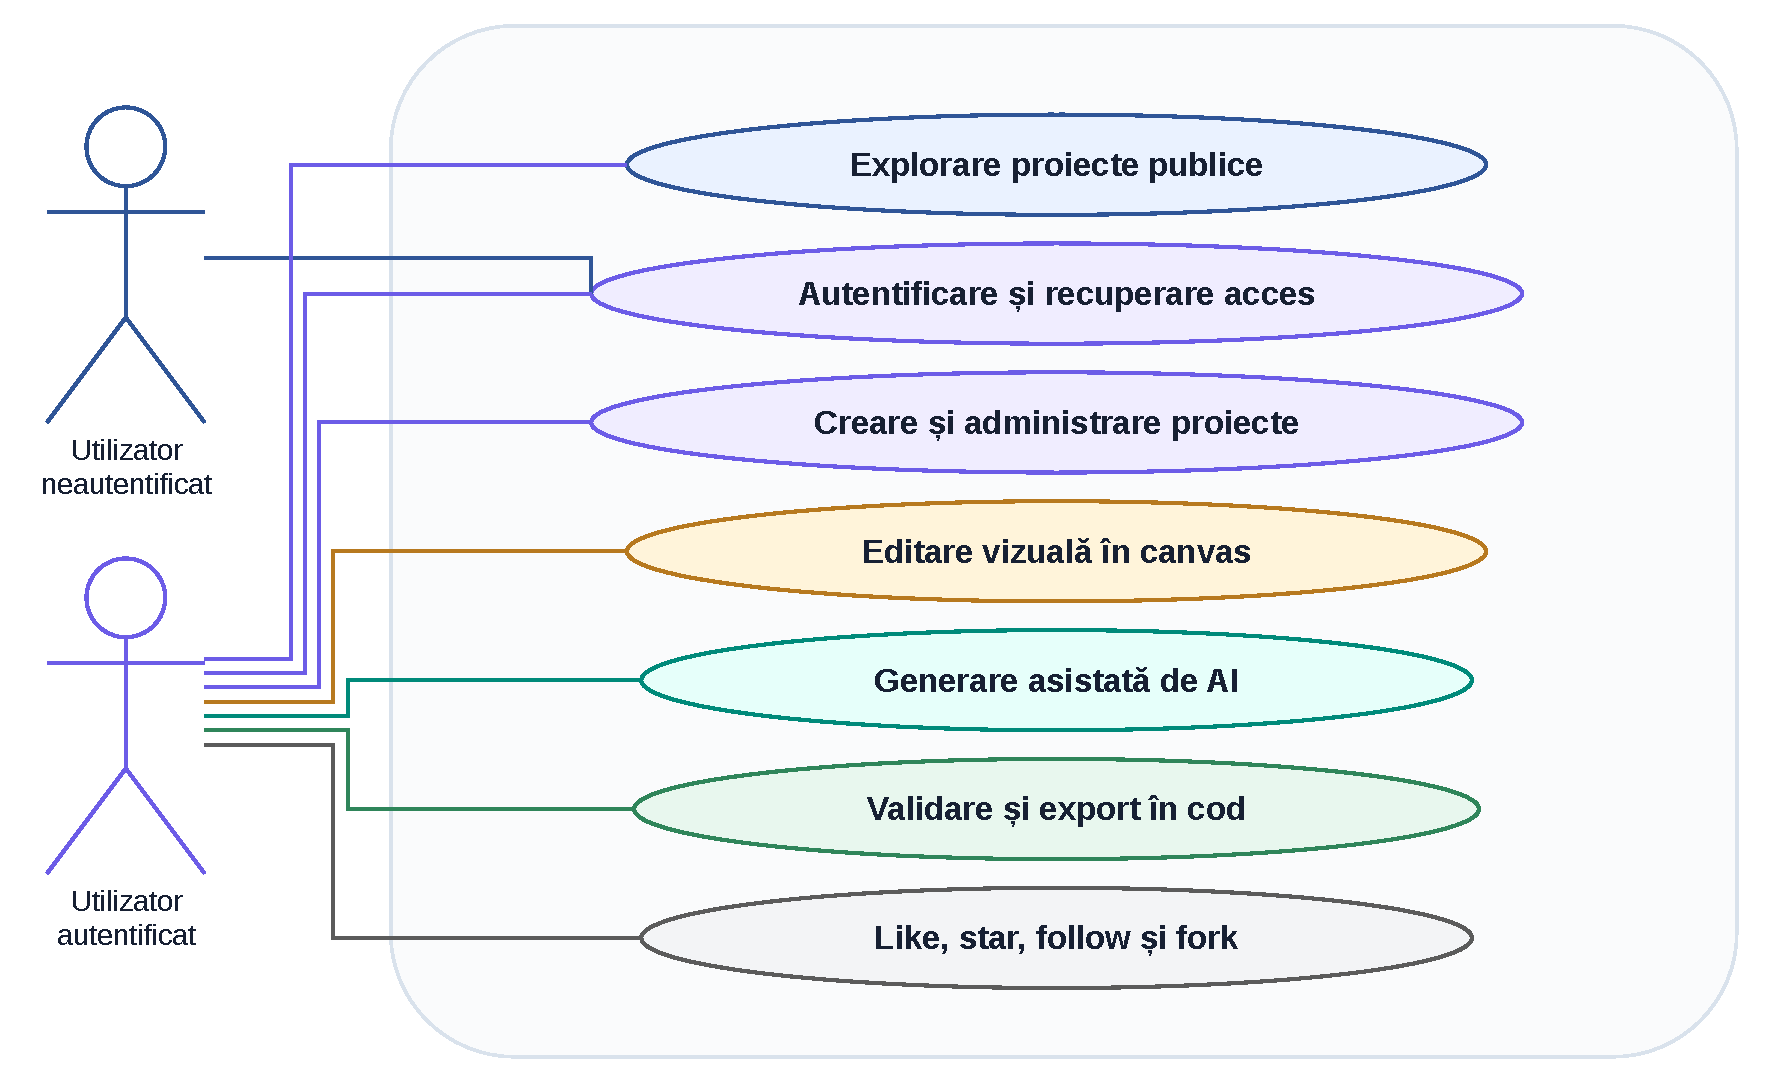
\includegraphics[width=0.97\textwidth]{diagrams/use-case-favigon.drawio.pdf}
  \caption{Diagrama de use-case simplificată pentru funcționalitățile principale din Favigon}
  \label{fig:use-case-favigon}
\end{figure}

\section{Scenarii principale de utilizare}

\subsection{Scenariul 1: creare și editare proiect}

Utilizatorul se autentifică, creează un proiect nou și ajunge în editorul canvas. Acolo poate adăuga elemente, poate crea pagini noi, poate modifica proprietăți și poate salva implicit progresul. La ieșire sau la schimbarea paginii, sistemul trebuie să se asigure că starea relevantă este persistată.

\subsection{Scenariul 2: generare asistată de AI}

Utilizatorul pornește de la un prompt și solicită generarea unei interfețe. Backend-ul trimite cererea către serviciul AI, primește etapele pipeline-ului și returnează rezultatul. Frontend-ul transformă structura obținută în elemente de canvas și permite utilizatorului să continue editarea manuală. Acest scenariu este important deoarece arată că AI-ul este integrat în fluxul editorului, nu separat de el.

\subsection{Scenariul 3: export în cod}

După ce proiectul ajunge într-o stare satisfăcătoare, utilizatorul cere validarea și exportul. Designul este convertit în reprezentarea intermediară, verificat și transmis motorului de conversie. Rezultatul este un set de fișiere pentru framework-ul ales. Acest scenariu justifică existența convertorului ca modul separat.

\subsection{Scenariul 4: distribuire și reutilizare}

Un utilizator publică un proiect, iar alt utilizator îl descoperă în explore sau pe profilul autorului. Poate să îl aprecieze, să îl salveze sau să îl fork-uiască. În acest fel, proiectul capătă și o dimensiune de comunitate, nu rămâne doar un document privat.

\section{Arhitectura generală}

La nivel înalt, sistemul este împărțit în frontend, backend, bază de date și servicii externe. Frontend-ul Angular gestionează interfața, rutarea și starea locală a editorului. Backend-ul ASP.NET Core expune endpoint-uri REST și coordonează logica de aplicație. PostgreSQL stochează datele persistente. Serviciile externe includ OpenAI API pentru generare și Cloudflare Tunnel pentru expunere controlată. Arhitectura logică rezultată este redată în Figura~\ref{fig:arhitectura-generala}.

\begin{figure}[H]
  \centering
  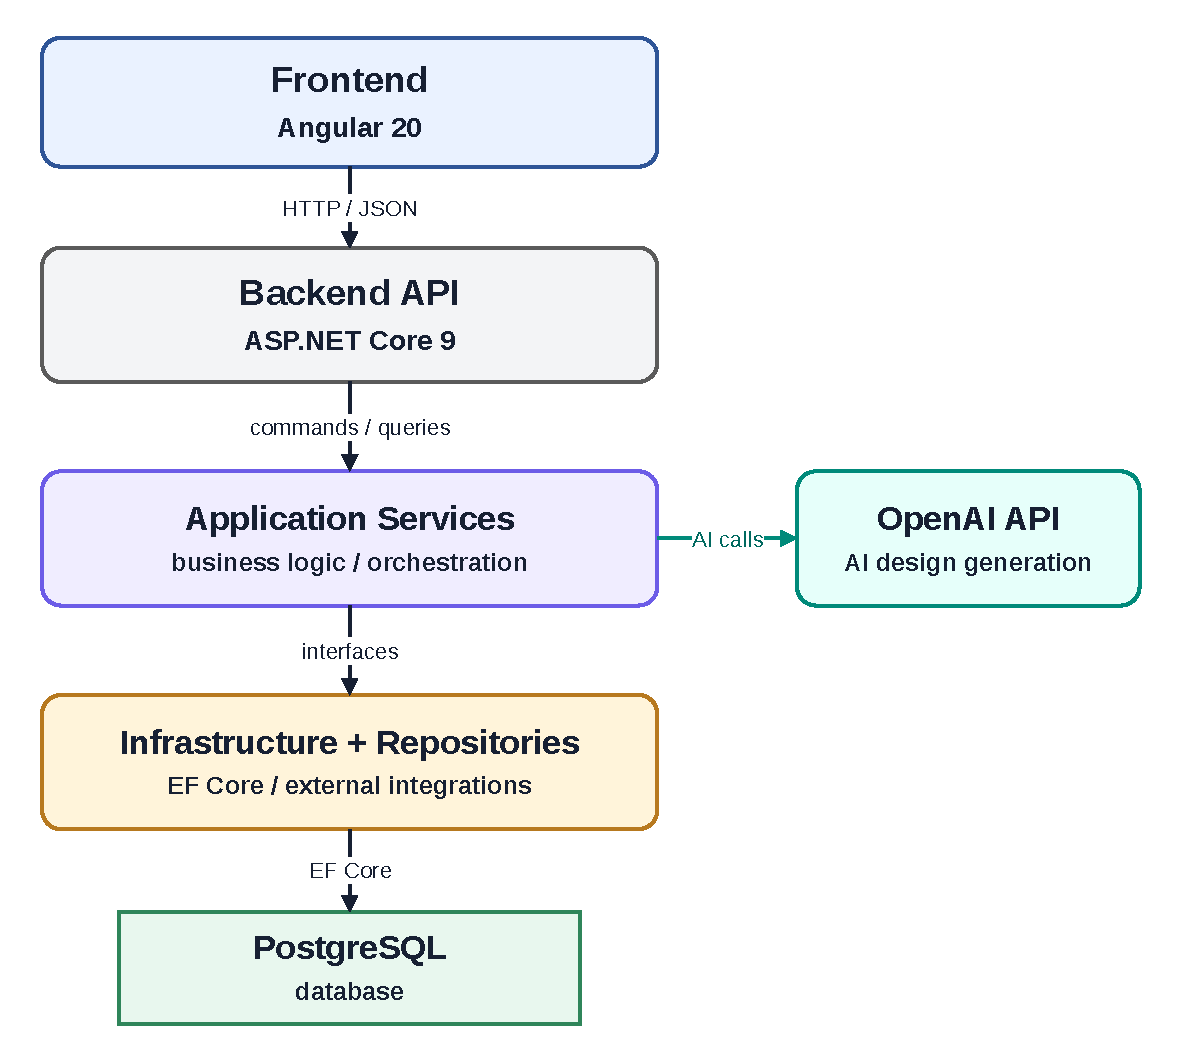
\includegraphics[width=0.92\textwidth]{diagrams/arhitectura-generala.drawio.pdf}
  \caption{Arhitectura logică generală a sistemului}
  \label{fig:arhitectura-generala}
\end{figure}

Această împărțire nu este doar una de prezentare. Ea se regăsește concret în structura soluției backend: proiectele `Favigon.API`, `Favigon.Application`, `Favigon.Infrastructure`, `Favigon.Domain`, `Favigon.Converter` și `Favigon.Tests`. Fiecare are un rol clar, iar motorul de conversie este separat explicit deoarece are propriile reguli și propria logică de transformare.

\section{Organizarea backend-ului pe straturi}

La nivel de backend, fluxul tipic al unei cereri este:

\begin{enumerate}[leftmargin=1.5cm]
  \item controller-ul primește cererea HTTP și verifică aspectele de intrare;
  \item serviciul de aplicație aplică logica de business;
  \item repository-ul sau adaptorul extern execută persistența sau integrarea necesară;
  \item rezultatul este mapat și întors către client.
\end{enumerate}

Această structură reduce riscul ca un controller să devină prea încărcat. De exemplu, un endpoint din `ProjectsController` nu decide singur cum se construiește un slug, cum se șterg asset-urile sau cum se tratează un fork. Toate acestea sunt delegate către `ProjectService`, care la rândul lui colaborează cu repository-ul și cu storage-ul pentru assets.

Avantajul acestei structuri este vizibil și în testare. Pentru că serviciile sunt relativ bine delimitate, ele pot fi verificate independent de transportul HTTP. De aceea, în proiect există teste directe pentru `AuthService`, `ProjectService`, `UserService` și `ConverterEngine`, nu doar teste la nivel de controller.

Aceeași organizare poate fi interpretată și printr-o lentilă apropiată de \textit{clean architecture}. Regulile esențiale ale produsului și reprezentările interne trebuie să rămână în centru, iar infrastructura, transportul HTTP și integrarea cu servicii externe trebuie să depindă de acest nucleu, nu invers. Figura~\ref{fig:clean-backend} sintetizează această idee pentru backend-ul Favigon.

\begin{figure}[H]
  \centering
  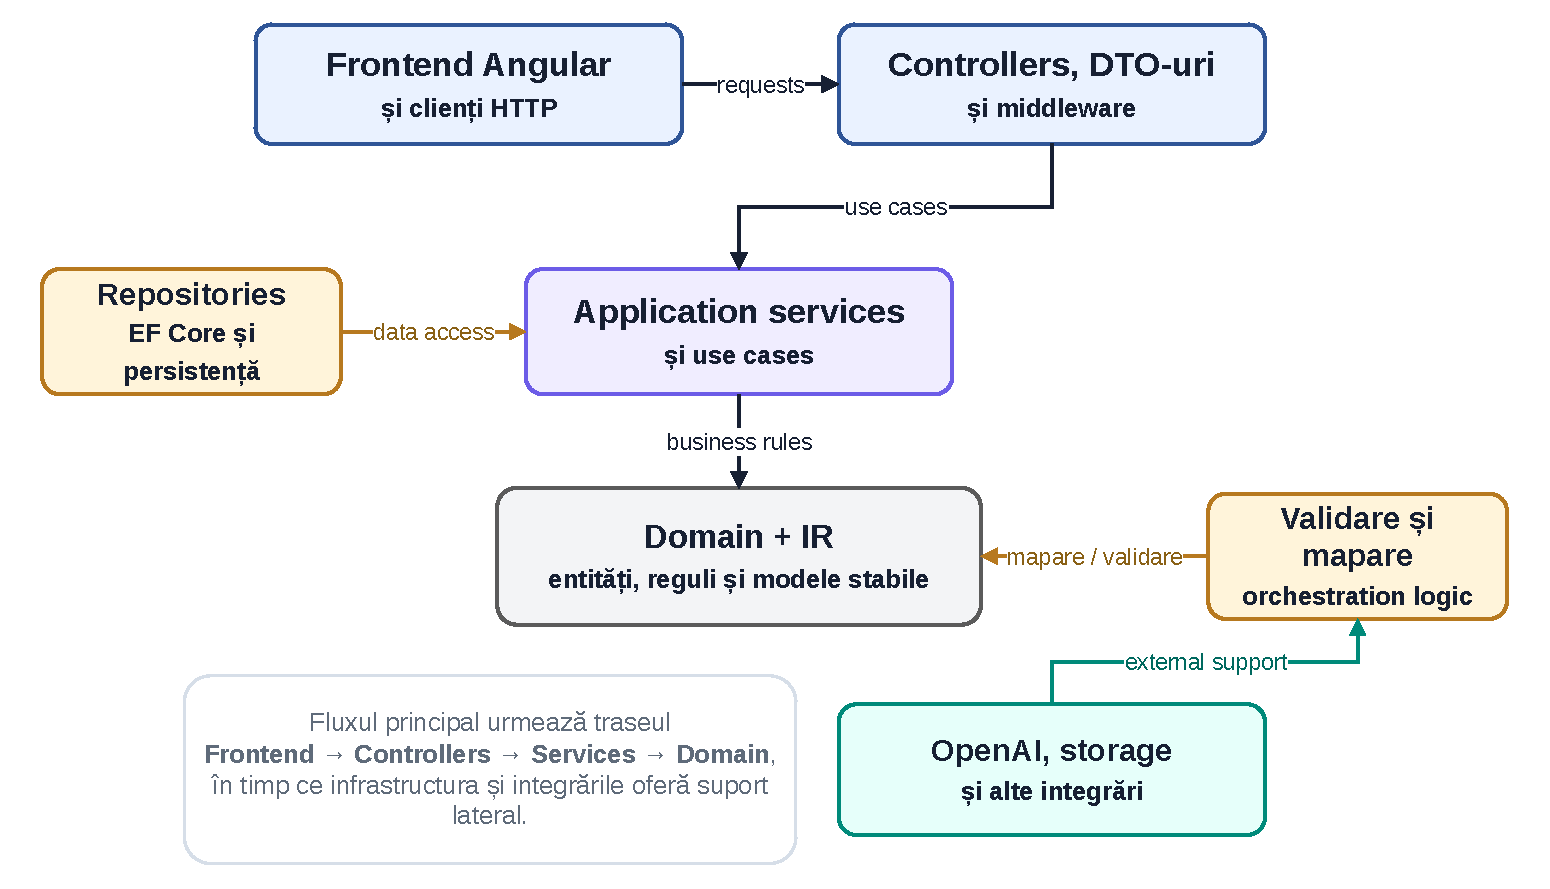
\includegraphics[width=0.95\textwidth]{diagrams/clean-backend.drawio.pdf}
  \caption{Vedere de tip clean architecture pentru backend-ul Favigon}
  \label{fig:clean-backend}
\end{figure}

\section{Organizarea frontend-ului pe feature-uri}

Frontend-ul este organizat în jurul conceptelor `core`, `shared` și `features`. `core` conține modelele, serviciile API, interceptorii și utilitarele globale. `shared` conține componente reutilizabile. `features` grupează zonele funcționale ale aplicației: autentificare, canvas, explore, profil, settings și stars.

Această structură este potrivită pentru proiect deoarece cea mai mare complexitate este concentrată într-un singur feature, anume `canvas`. În loc să împrăștii logica editorului în toată aplicația, serviciile, mapper-ele și utilitarele specifice au fost păstrate aproape de acest feature. În practică, această alegere a redus numărul de dependențe surpriză și a făcut fluxul de lucru mai ușor de urmărit.

\section{Modelul de date conceptual}

Din punct de vedere conceptual, modelul de date are câteva entități centrale: utilizatorul, proiectul, conturile externe legate de utilizator, relațiile de follow dintre utilizatori și relațiile de like sau bookmark dintre utilizatori și proiecte. Designul efectiv al unui proiect este stocat ca JSON în cadrul proiectului, deoarece structura lui este prea flexibilă pentru o modelare exclusiv relațională. Vederea conceptuală simplificată apare în Figura~\ref{fig:model-conceptual}.

\begin{figure}[H]
  \centering
  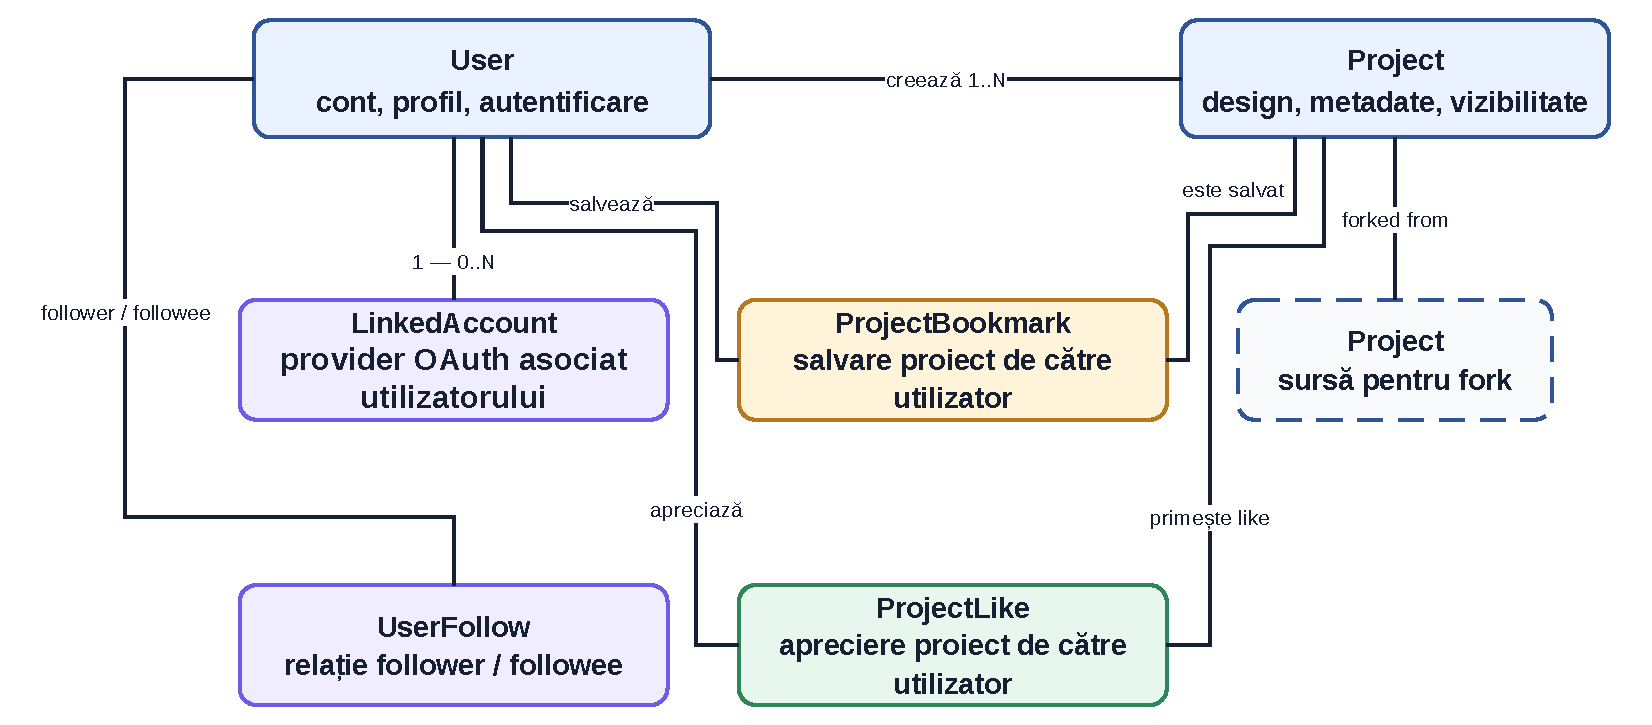
\includegraphics[width=0.94\textwidth]{diagrams/model-conceptual.drawio.pdf}
  \caption{Model conceptual simplificat al datelor principale}
  \label{fig:model-conceptual}
\end{figure}

Din cod se observă și câteva decizii importante. Proiectul are câmpuri pentru `Slug`, `IsPublic`, `ThumbnailDataUrl`, `ViewCount` și `ForkedFromProjectId`. Utilizatorul are câmpuri pentru `HasPassword`, `IsTwoFactorEnabled`, datele de resetare a parolei și date temporare pentru fluxul 2FA. Aceste câmpuri arată că modelul este orientat clar spre un produs complet, nu doar spre stocarea unui desen.

Pentru a trece de la nivelul de domeniu la nivelul de implementare, Figura~\ref{fig:erd-fizic} prezintă un ERD simplificat extras din configurația Entity Framework Core. El evidențiază entitățile persistente, cheile principale și relațiile care merită discutate la nivel de licență.

\begin{figure}[H]
  \centering
  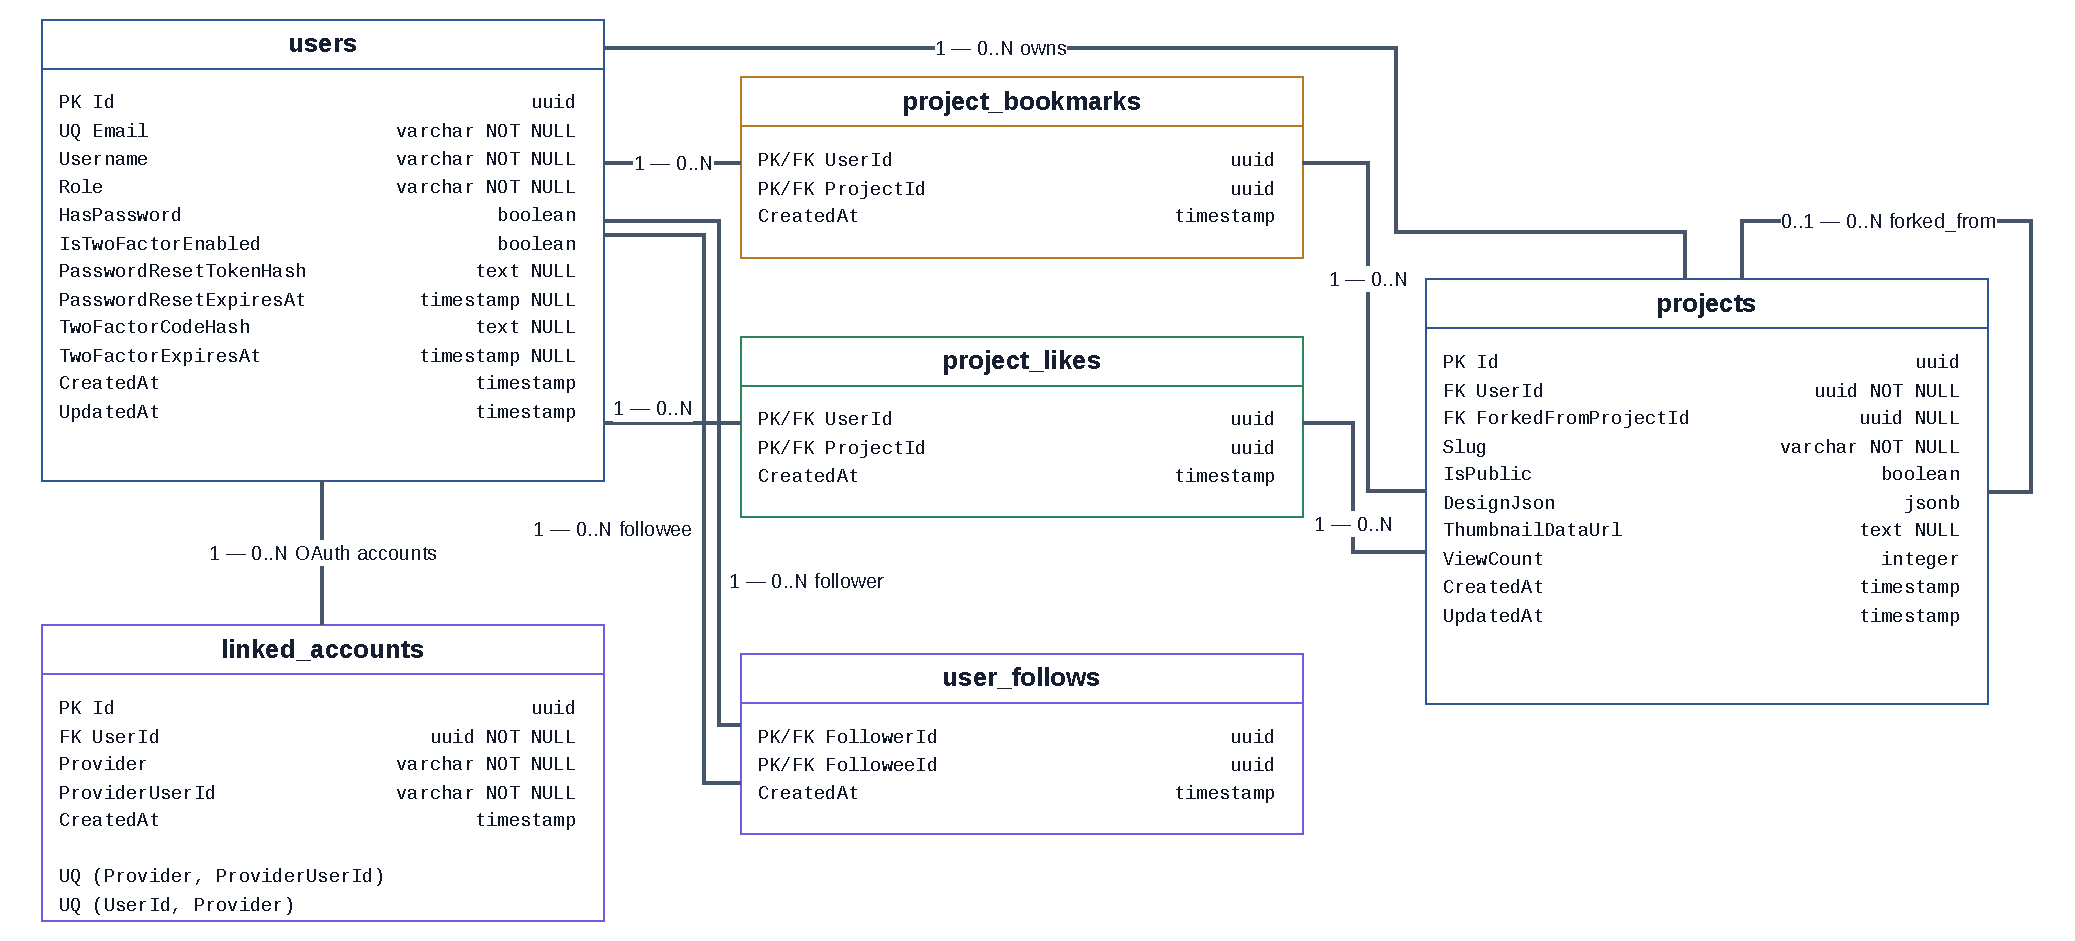
\includegraphics[width=\textwidth]{diagrams/erd-fizic.drawio.pdf}
  \caption{ERD simplificat pentru schema fizică a bazei de date}
  \label{fig:erd-fizic}
\end{figure}

ERD-ul scoate în evidență și câteva constrângeri importante din implementare: unicitatea email-ului pentru utilizatori, unicitatea conturilor externe pe perechile \texttt{(Provider, ProviderUserId)} și \texttt{(UserId, Provider)}, cheile compuse pentru relațiile sociale și autoreferința \texttt{ForkedFromProjectId} din \texttt{projects}. Astfel, schema nu stochează doar resurse izolate, ci și legăturile necesare pentru reutilizare, explorare și trasabilitatea fork-urilor.

Această structură arată explicit și compromisul de modelare adoptat în proiect. Datele cu structură stabilă, cum sunt identitatea utilizatorului, relațiile sociale și metadatele proiectelor, rămân relaționale. În schimb, documentul efectiv al interfeței este păstrat compact în \texttt{DesignJson}, deoarece arborele de elemente, stiluri și layout-uri este prea flexibil pentru a fi mapat eficient în tabele relaționale fine. În plus, timestamp-urile \texttt{CreatedAt} și \texttt{UpdatedAt} sunt menținute automat în contextul de persistență, ceea ce reduce riscul de inconsistență între creare, actualizare și export ulterior.

\section{Fluxurile principale}

\subsection{Fluxul de autentificare}

Fluxul de autentificare începe cu un request către `AccountController`, este procesat în `AuthService`, iar la final backend-ul emite cookie-urile necesare. Dacă utilizatorul are 2FA activ, autentificarea este împărțită în două etape: validarea credențialelor și validarea codului temporar. Această separare este reflectată și în cod, prin token-ul temporar specific fluxului 2FA.

\subsection{Fluxul de editare}

La deschiderea unui proiect, frontend-ul încarcă datele proiectului și apoi designul asociat. `CanvasPersistenceService` coordonează persistarea automată și sincronizarea thumbnail-ului, iar starea editorului este împărțită între mai multe servicii specializate. Din punct de vedere al utilizatorului, totul ar trebui să pară unitar. Din punct de vedere intern, însă, fluxul este descompus în pași mai mici tocmai pentru a păstra controlul asupra lui.

\subsection{Fluxul de export}

Pentru export, editorul produce reprezentarea intermediară, apoi o trimite către backend prin `ConverterController`. `ConverterService` validează structura și apelează `ConverterEngine`, care generează fișierele pentru framework-ul ales. Acest flux este important deoarece justifică separarea convertorului într-un proiect distinct.

\subsection{Fluxul AI}

Pentru generare, frontend-ul trimite un prompt către `AiDesignController`. Backend-ul poate răspunde fie clasic, fie prin streaming SSE. În spate, `AiPipelineService` parcurge fazele de intenție, structură și stil, iar rezultatul final este transformat în date pe care frontend-ul le poate integra în editor.

\section{Decizii de proiectare care au influențat cel mai mult implementarea}

Privind retrospectiv, există câteva decizii de proiectare care au avut impact major asupra întregului proiect.

Prima decizie a fost separarea clară între canvas și codul final exportat. O abordare bazată pe editarea directă a HTML-ului sau a DOM-ului ar fi produs probabil un sistem mai fragil și mai greu de extins.

A doua decizie a fost tratarea AI-ului ca pe un subsistem controlabil, nu ca pe o cutie neagră. De aici rezultă atât folosirea JSON Schema, cât și împărțirea pipeline-ului.

A treia decizie a fost păstrarea logicii editorului în servicii specializate. Fără acest pas, componenta principală de canvas ar fi devenit foarte repede imposibil de întreținut.

A patra decizie a fost folosirea unei baze relaționale pentru metadate și a unui câmp JSON pentru design. Deși este un compromis, el s-a dovedit eficient pentru tipul de informații gestionate.

\section{Concluzii intermediare}

În urma analizei și proiectării, sistemul rezultat are o formă coerentă atât la nivel de produs, cât și la nivel tehnic. Cerințele au fost traduse într-o arhitectură cu straturi clare, actori bine definiți, fluxuri importante și un model de date adaptat problemei.

Capitolul următor trece de la această vedere de ansamblu la implementarea concretă a platformei: autentificare, proiecte, funcții sociale și editorul canvas.








\chapter{Implementarea platformei Favigon}

\section{Privire de ansamblu asupra implementării}

După etapa de proiectare, implementarea efectivă a platformei a urmărit aceeași idee centrală: fiecare zonă importantă a produsului trebuie să aibă responsabilități clare și puncte de integrare ușor de urmărit. În practică, asta a însemnat că nu a fost dezvoltat întâi un editor izolat și abia apoi restul produsului, ci aplicația a evoluat ca întreg.

Mai exact, partea de autentificare, management de proiecte și persistare a fost dezvoltată relativ devreme, pentru că fără ele editorul ar fi rămas un demo local. Apoi au fost consolidate editorul canvas și suportul pentru export. Într-o etapă ulterioară au fost integrate fluxurile AI și a fost extinsă componenta socială, astfel încât proiectele să poată fi nu doar create, ci și publicate, descoperite și reutilizate.

Rezultatul este o aplicație în care modulele sunt diferite ca rol, dar strâns legate între ele. De exemplu, editorul depinde de proiecte, proiectele depind de autentificare, generarea AI depinde de editor și de modelul intermediar, iar funcțiile sociale depind de modelul relațional al utilizatorilor și proiectelor.

\section{Rutare și pornirea aplicației frontend}

Configurația frontend-ului este definită în \texttt{ApplicationConfig}, prin \texttt{provideRouter}, \texttt{provideHttpClient} cu interceptori și \texttt{provideAnimations}. Alegerea este în linie cu stilul modern Angular bazat pe componente standalone. Din punct de vedere practic, ea reduce nevoia unor module centrale voluminoase și face mai clară relația dintre rutare, infrastructura HTTP și comportamentul global al aplicației.

Un alt detaliu util este activarea \texttt{provideZoneChangeDetection} cu \texttt{eventCoalescing}. Pentru un produs cu editor vizual, optimizarea este relevantă deoarece reduce numărul de actualizări declanșate de evenimente succesive și ajută la păstrarea unei interfețe mai fluide în scenarii de drag, selecție sau input repetat.

Rutarea este organizată astfel încât paginile principale să fie încărcate lazy și protejate diferențiat. Ruta rădăcină nu trimite utilizatorul într-o pagină statică, ci încearcă să încarce utilizatorul curent și redirecționează dinamic fie spre profilul acestuia, fie spre \texttt{/login}. În plus, editorul canvas folosește un \textit{canDeactivate guard} care forțează flush-ul persistenței înainte de părăsirea paginii, ceea ce leagă direct infrastructura de navigare de cerința de robusteză a autosave-ului.

\begin{table}[H]
  \centering
  \caption{Rute frontend principale și rolul lor în aplicație}
  \label{tab:rute-frontend}
  \renewcommand{\arraystretch}{1.15}
  \begin{tabularx}{\textwidth}{>{\RaggedRight\arraybackslash}p{4.2cm}>{\RaggedRight\arraybackslash}p{4.1cm}Y}
    \toprule
    \textbf{Rută} & \textbf{Scop} & \textbf{Observații de acces / navigare} \\
    \midrule
    \path{/login} & autentificare în sistem & \texttt{loginEntryGuard}; evită revenirea inutilă la login \\
    \path{/reset-password} & recuperare acces & rută publică pentru resetarea parolei \\
    \path{/project/:slug} & editorul canvas & \texttt{authGuard} și \texttt{canDeactivate} pentru flush \\
    \path{/project/:slug/preview} & previzualizare HTML & necesită autentificare și randare separată \\
    \path{/explore} & descoperire de proiecte & punct de intrare în zona socială \\
    \path{/settings} & configurări de profil & disponibilă doar utilizatorului autentificat \\
    \path{/stars} & proiecte salvate & afișează bookmark-urile proprii \\
    \path{/:username} & profil public / propriu & destinație implicită după încărcarea sesiunii \\
    \bottomrule
  \end{tabularx}
\end{table}

Interacțiunea dintre rutare și infrastructura HTTP este completată de doi interceptori importanți: unul pentru trimiterea credențialelor către API și altul pentru încercarea automată de refresh atunci când sesiunea curentă expiră. Din punct de vedere al utilizatorului, această logică face ca aplicația să pară mai continuă și mai coerentă; din punct de vedere tehnic, ea mută comportamentele repetitive într-un strat transversal, în loc să fie duplicate în fiecare pagină sau serviciu.

\section{Modulul de autentificare și profil}

\subsection{Fluxurile de bază}

Modulul de autentificare este implementat în jurul `AccountController` și al serviciului `AuthService`. La nivel de API există endpoint-uri pentru register, login, logout, refresh, resetare parolă, setare parolă, schimbare parolă, autentificare prin GitHub și Google, precum și pentru activarea sau dezactivarea autentificării în doi pași.

Pe partea de backend, `AuthService` face mai mult decât o simplă verificare de credențiale. El normalizează datele de intrare, verifică unicitatea utilizatorului, gestionează hash-uirea parolei, tratează fluxurile OAuth, construiește token-urile JWT și emite un token temporar pentru etapa intermediară a autentificării în doi pași. În plus, aceeași zonă gestionează și resetarea parolei prin token transmis prin email.

Din punct de vedere al produsului, autentificarea nu este tratată ca o singură operație de tip ``email + parolă''. În practică, utilizatorii pot intra în sistem prin mai multe căi și pot avea conturi legate la furnizori diferiți. Din acest motiv există și entitatea `LinkedAccount`, folosită pentru asocierea unui utilizator local cu identități externe.

\subsection{JWT în cookie și refresh token}

O decizie importantă a fost transportul token-ului de acces prin cookie HTTP only. În implementare, controller-ul nu întoarce token-ul către frontend pentru stocare manuală în `localStorage`, ci îl plasează în cookie-ul `jwt`. Refresh token-ul este păstrat separat, într-un cookie dedicat cu path limitat la endpoint-ul de refresh.

Această alegere simplifică partea de client și reduce expunerea unor date sensibile în codul din browser. În același timp, introduce și obligația de a trata atent expirațiile și reînnoirea sesiunii. De aceea, în frontend există și interceptorul de refresh, care încearcă revalidarea sesiunii când întâlnește un răspuns care indică expirarea token-ului de acces.

\subsection{Autentificarea în doi pași}

În cadrul proiectului, 2FA este implementat prin cod temporar trimis prin email. La prima vedere, acesta nu este cel mai avansat model posibil, dar pentru scopul aplicației este o soluție rezonabilă și ușor de demonstrat. În plus, implementarea este structurată destul de curat: există flux separat pentru activare, dezactivare și verificare la login, iar token-ul temporar pentru sesiunea de autentificare incompletă este diferit de token-ul normal de acces.

Această funcționalitate nu rămâne la nivel de extensie izolată. Ea este integrată atât în serviciul de autentificare, cât și în controller, în opțiuni și în fluxul de UI, ceea ce îi conferă rolul unei măsuri reale de securitate operațională.

\subsection{Profilul utilizatorului}

Pe lângă autentificare, utilizatorul își poate administra profilul: nume afișat, bio, imagine și legături OAuth. `UsersController` expune endpoint-uri pentru profilul curent, încărcarea imaginii de profil, căutarea de utilizatori și vizualizarea profilurilor publice. În plus, există endpoint-uri pentru follow și unfollow, precum și pentru listele de followers și following.

Această parte a aplicației are un rol dublu. Pe de o parte este o funcționalitate de produs normală. Pe de altă parte, ea oferă baza pentru zona socială și pentru ideea că proiectele au autori, pot fi urmărite și pot circula între utilizatori.

\section{Gestionarea proiectelor}

\subsection{Ciclul de viață al proiectelor}

`ProjectService` este una dintre cele mai importante piese din backend, deoarece concentrează logica legată de proiecte. El gestionează crearea proiectului, actualizarea metadatelor, ștergerea, salvarea designului, salvarea thumbnail-ului, upload-ul de imagini, bookmark-urile, like-urile și operația de fork.

La creare, proiectul primește un slug unic derivat din nume. La modificare, dacă numele se schimbă, slug-ul este recalculat. La ștergere, serviciul se ocupă și de curățarea asset-urilor asociate. Acest detaliu este important deoarece evită acumularea de fișiere orfane și arată că proiectul nu tratează persistența doar la nivel de bază de date, ci și la nivelul fișierelor încărcate.

\subsection{Persistarea designului}

Pentru design-ul propriu-zis al unui proiect, backend-ul păstrează JSON-ul serializat în câmpul `DesignJson` al entității `Project`. Pe frontend, `CanvasPersistenceService` coordonează încărcarea, transformarea și salvarea acestui document.

Un aspect important este că salvarea nu este exclusiv manuală. Editorul folosește persistare automată cu debounce și mecanisme de flush atunci când utilizatorul părăsește pagina sau proiectul trebuie sincronizat imediat. Acest comportament este important pentru UX. Dacă utilizatorul lucrează într-un editor de design și trebuie să apese explicit \textit{Save} după fiecare pas important, experiența devine artificială și fragilă.

În implementare, persistarea automată este tratată explicit prin parametri observabili în cod: schimbările relevante programează o salvare după 500 ms, flush-ul așteaptă cel mult 4 s finalizarea persistenței, iar la erori temporare se folosesc până la 4 reîncercări cu backoff exponențial pornind de la 2 s. Serviciul gestionează separat stările de \textit{isSaving}, persistarea la ieșirea din pagină și generarea de thumbnail-uri după perioade scurte de inactivitate. Aceste detalii transformă editorul dintr-un demo interactiv într-un subsistem care poate susține utilizare repetată.

\subsection{Thumbnail și asset-uri}

Fiecare proiect poate avea și thumbnail. În editor, thumbnail-ul este generat automat pornind din canvas, inclusiv printr-o variantă bazată pe `html2canvas`. Pe backend, fișierul este salvat separat, iar la update se invalidează vechiul `ThumbnailDataUrl` dacă este cazul.

În plus, proiectul suportă upload de imagini pentru asset-uri folosite în design. Validarea fișierelor se face în backend, iar stocarea este abstractizată printr-un serviciu dedicat. Această decizie a fost utilă pentru că a evitat legarea prea strânsă a logicii de proiecte de detaliile concrete ale fișierelor.

Un detaliu important, mai puțin vizibil în interfață, este ciclul de viață al asset-urilor. La resalvarea designului, backend-ul compară asset-urile prezente în documentul nou cu cele din versiunea anterioară și poate elimina resursele care au devenit orfane. În mod similar, la ștergerea unui proiect sau a unui cont, sunt curățate atât asset-urile proiectelor, cât și imaginea de profil a utilizatorului. Această zonă nu schimbă experiența vizuală în mod direct, dar este importantă pentru a arăta că aplicația tratează responsabil și consistența stocării de fișiere.

\section{Funcționalități sociale și explorare}

Componenta socială este construită peste fluxurile de explorare, proiecte și utilizatori, împreună cu serviciile și repository-urile aferente. În această zonă, utilizatorii pot vedea proiecte populare sau recomandate, pot descoperi alți utilizatori, pot aprecia proiecte, le pot salva și le pot reutiliza prin fork.

Deși această zonă nu este nucleul tehnic al lucrării, ea schimbă semnificativ caracterul produsului. Fără ea, Favigon ar fi rămas un editor personal. Cu ea, proiectul capătă logică de comunitate: există autori, conținut public, indicatori de interes și relații între utilizatori.

În implementare, `ExploreService` tratează separat trei fluxuri: proiecte \textit{trending}, proiecte recomandate și utilizatori sugerați. Pentru proiectele populare este folosit un set limitat de rezultate, potrivit pentru afișarea rapidă a conținutului public. Pentru recomandări, backend-ul verifică mai întâi dacă utilizatorul autentificat urmărește deja alte conturi; dacă da, încearcă să construiască un răspuns personalizat, iar dacă nu există bază suficientă sau utilizatorul este anonim, revine la o selecție generală de proiecte recente și relevante. Pentru sugestiile de persoane, serviciul returnează informații derivate precum numărul de urmăritori, numărul de proiecte publice și starea \textit{isFollowedByCurrentUser}. Această logică oferă zonei `explore` un comportament mai apropiat de un produs real decât de o simplă listă statică.

Operația de fork este deosebit de interesantă deoarece leagă partea socială de partea de producție. Când un utilizator face fork la un proiect public, sistemul creează un nou proiect privat pentru el, cu design-ul copiat și cu legătura către proiectul-sursă. Astfel, reutilizarea nu este doar conceptuală, ci concretă și trasabilă.

\begin{figure}[H]
  \centering
  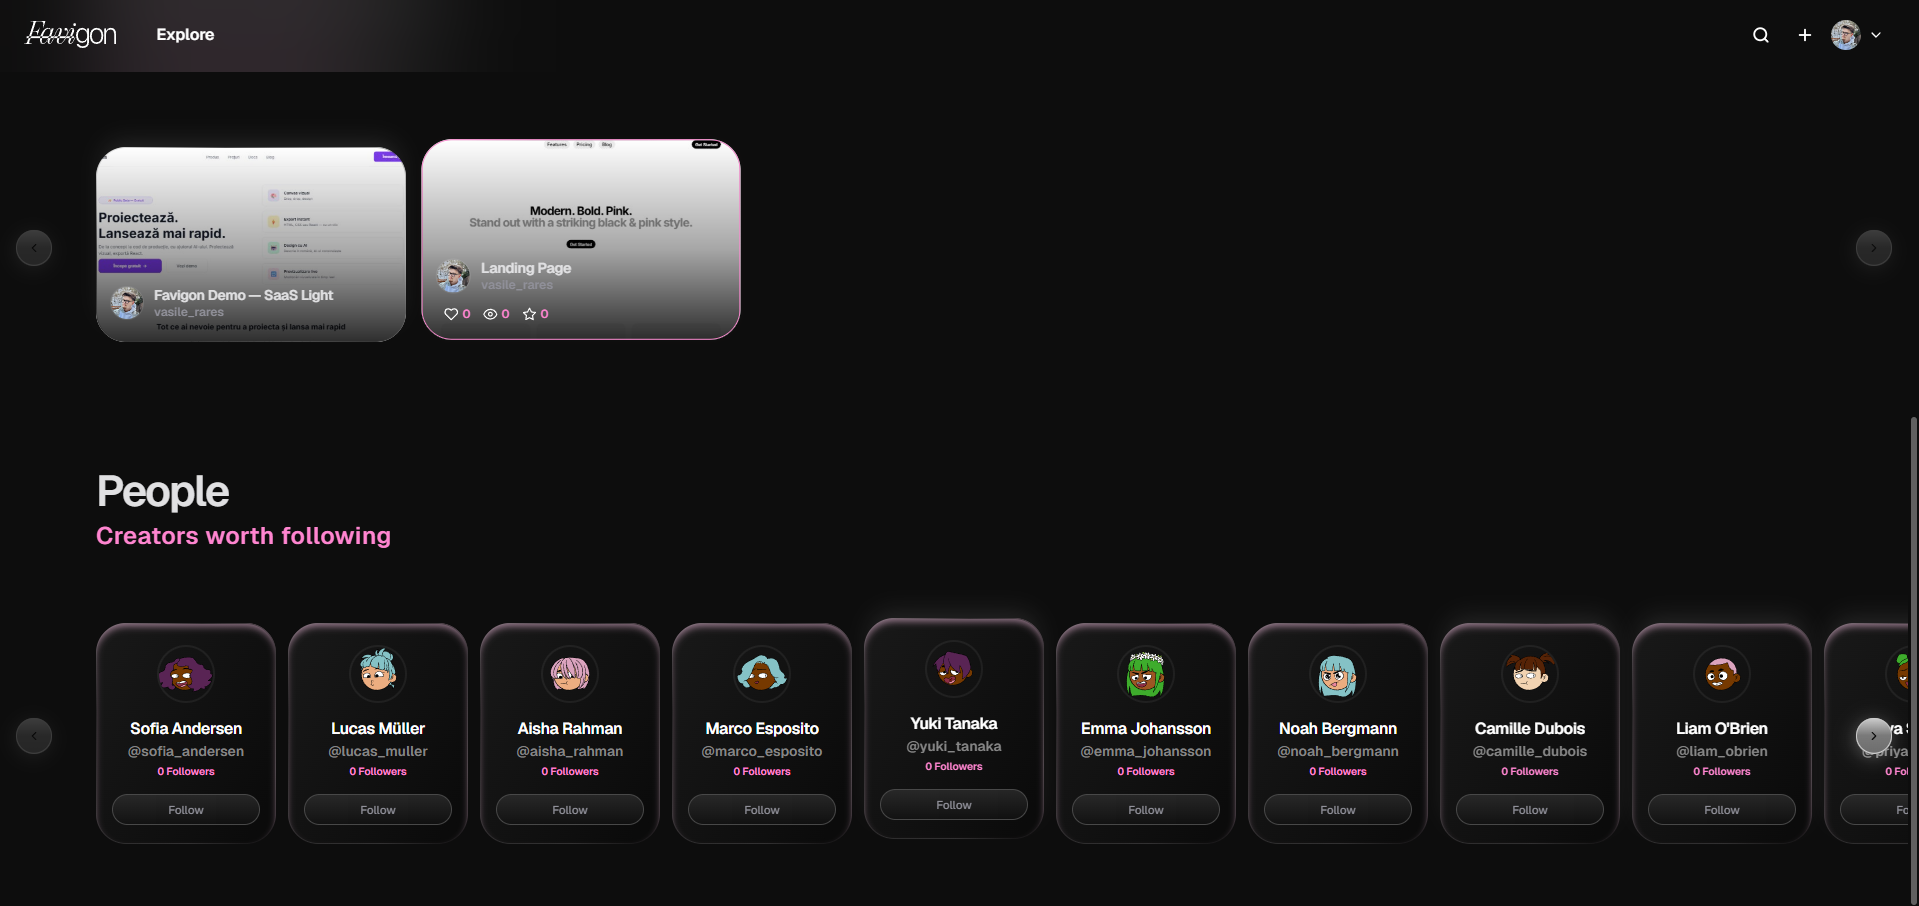
\includegraphics[width=0.96\textwidth]{images/explore_page.png}
  \caption{Interfața paginii Explore, cu proiecte publice și utilizatori sugerați}
  \label{fig:explore-page}
\end{figure}

\section{Suprafața API și distribuția responsabilităților}

Din perspectiva backend-ului, aplicația expune o suprafață REST suficient de largă încât să merite descrisă separat. În forma actuală, API-ul este împărțit în șase controllere principale. Unele acoperă autentificarea și profilul, altele gestionează proiectele și componenta socială, iar cele rămase tratează generarea asistată de AI și exportul în cod.

Distribuția responsabilităților pe controllere are un rol important în claritatea implementării. Zonele costisitoare sau sensibile, precum AI-ul și convertorul, sunt separate de ciclul de viață al proiectelor. În același timp, controllerele de produs, cum sunt cele pentru proiecte și utilizatori, pot rămâne focalizate pe resursele pe care le gestionează. Astfel, API-ul nu devine o colecție arbitrară de endpoint-uri, ci o hartă destul de coerentă a capabilităților aplicației.

\begin{table}[H]
  \centering
  \caption{Controllere API și responsabilitățile lor dominante}
  \label{tab:controllere-api}
  \renewcommand{\arraystretch}{1.15}
  \begin{tabularx}{\textwidth}{>{\RaggedRight\arraybackslash}p{2.9cm}>{\RaggedRight\arraybackslash}p{5.1cm}Y}
    \toprule
    \textbf{Controller} & \textbf{Resurse / operații principale} & \textbf{Observații utile} \\
    \midrule
    Account & autentificare, sesiune, parole, OAuth, 2FA & concentrează logica de intrare în sistem \\
    Projects & CRUD proiecte, design, asset-uri, reacții, fork & controllerul cel mai bogat din zona de produs \\
    Users & profil curent/public, follow, linked accounts & leagă identitatea utilizatorului de zona socială \\
    Explore & trending, recomandări și sugestii de utilizatori & pune în valoare date agregate și filtrate, nu doar resurse brute \\
    AI design & generare directă, streaming, pipeline pe faze & include atât răspuns sincron, cât și SSE incremental \\
    Converter & validare IR, export HTML/React/Angular, multi-page & separă clar validarea de generarea finală \\
    \bottomrule
  \end{tabularx}
\end{table}

În implementare se observă și diferențierea infrastructurală a acestor zone. Controllerul AI este protejat atât prin autorizare, cât și prin politica dedicată de rate limiting \texttt{ai}. Controllerul de conversie are propria politică \texttt{converter}, iar \texttt{ProjectsController} aplică și limite diferite de dimensiune pentru upload de imagini, salvare design, flush și thumbnail. Aceste detalii arată că separarea controllerelor nu este doar conceptuală, ci are și efecte practice asupra securității, costului și fiabilității API-ului.

Dacă diagrama de arhitectură din capitolul precedent arată straturile mari, Figura~\ref{fig:backend-structural} coboară un nivel și sintetizează colaborarea dintre clasele și serviciile dominante din fluxurile AI și export. Nu este o diagramă exhaustivă a întregului backend, ci o vedere structurală orientată pe subsistemele cele mai relevante pentru contribuția tehnică a lucrării.

\begin{figure}[H]
  \centering
  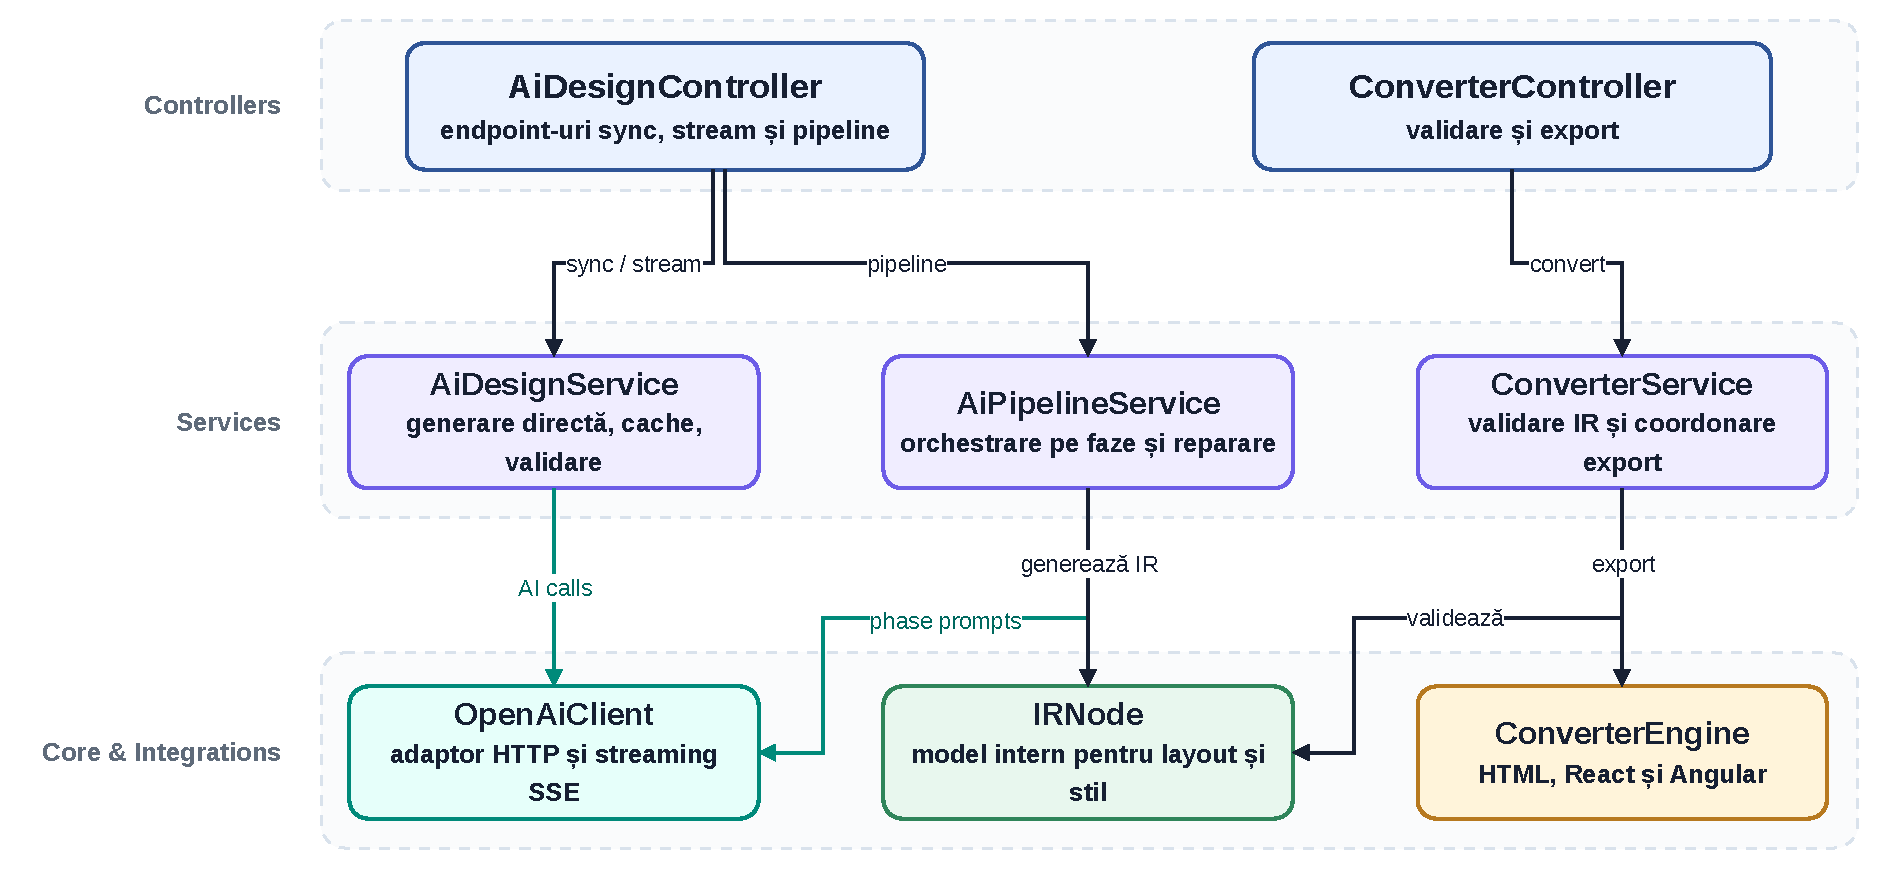
\includegraphics[width=0.96\textwidth]{diagrams/backend-structural.drawio.pdf}
  \caption{Vedere structurală simplificată a principalelor clase și servicii backend}
  \label{fig:backend-structural}
\end{figure}

\section{Editorul canvas}

\subsection{Rolul editorului în întregul produs}

Editorul canvas este zona cea mai complexă din frontend și, în mod realist, centrul aplicației. În jurul lui gravitează generarea AI, persistarea, exportul și o mare parte din interacțiunile vizuale ale utilizatorului. În implementare, pagina principală a editorului (`CanvasPage`) este o componentă mare, dar ea funcționează mai mult ca punct de orchestrare decât ca loc în care se află toată logica.

Practic, componenta injectează o suită întreagă de servicii: stare editor, viewport, istoric, clipboard, gesturi, context menu, persistare, generare, manager de pagini, stilizare DOM și altele. Separarea urmărește principiile interacțiunii de tip \textit{direct manipulation}, unde utilizatorul operează pe obiecte vizibile, primește feedback imediat și poate reveni rapid asupra acțiunilor \cite{shneiderman1983direct}. În același timp, păstrarea unui model intern separat de suprafața vizuală apropie editorul de direcțiile discutate în literatura despre combinarea editării directe cu reprezentări programabile \cite{chugh2016programmatic}. Principalele servicii implicate sunt sintetizate în Figura~\ref{fig:canvas-servicii}.

\begin{figure}[H]
  \centering
  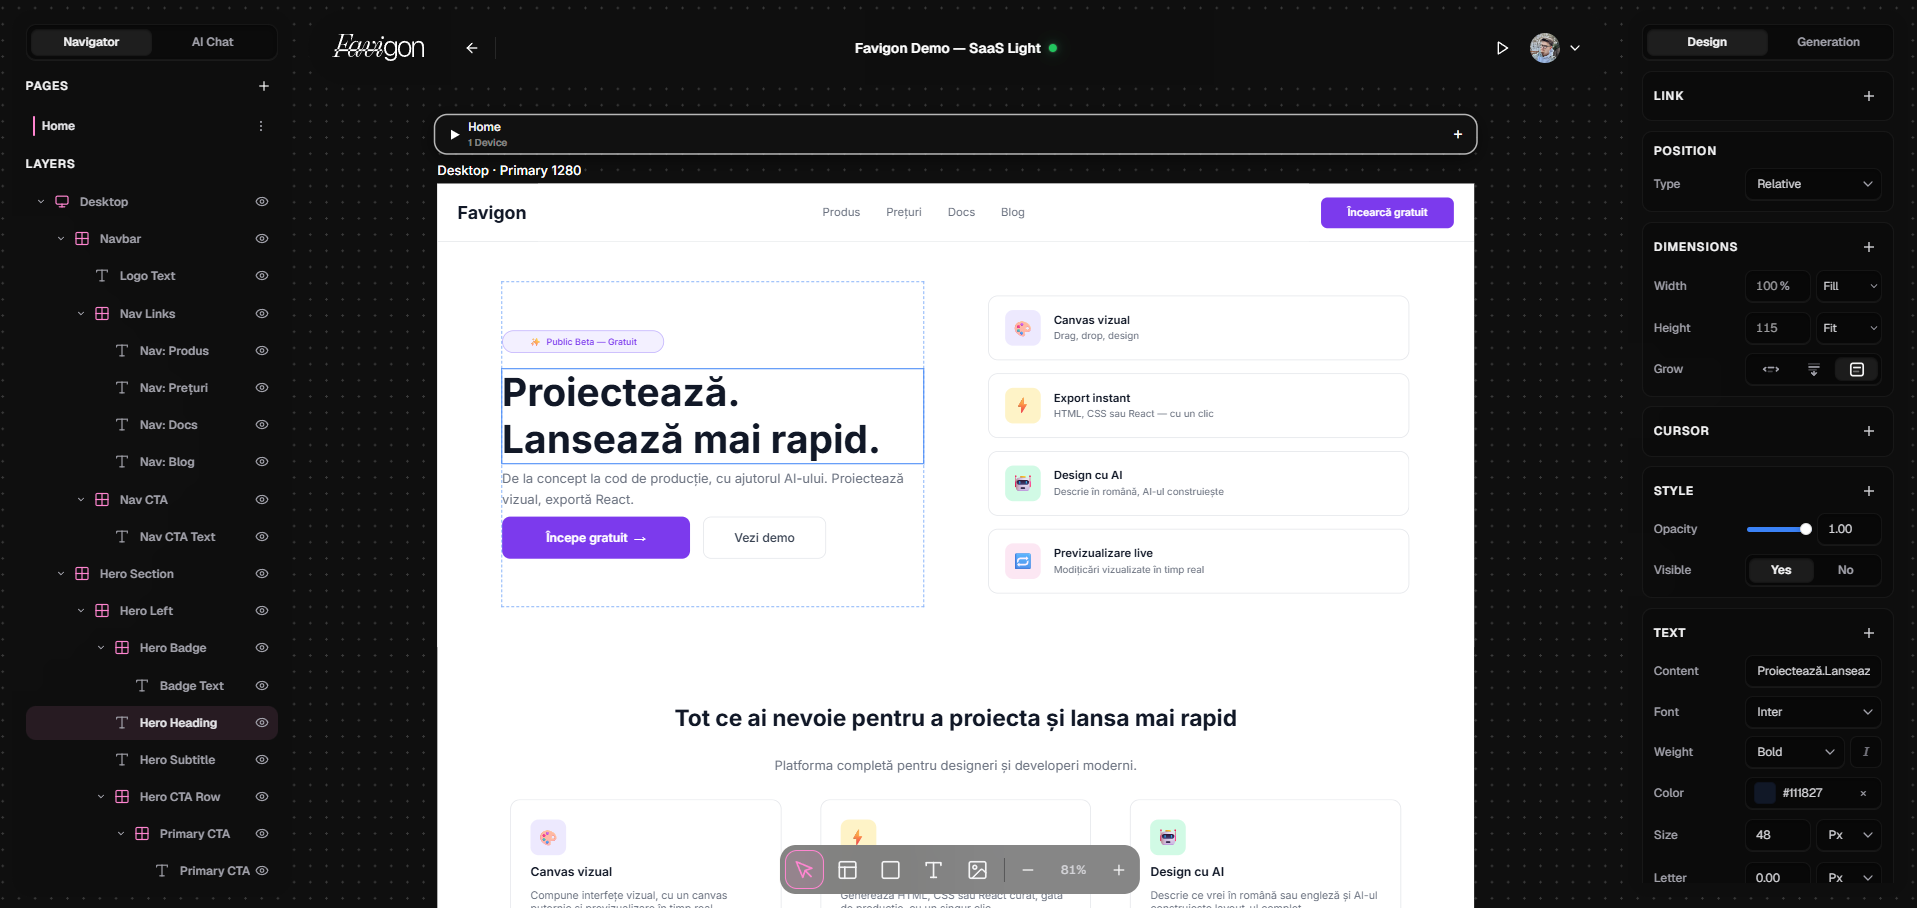
\includegraphics[width=0.96\textwidth]{images/canvas_editor.png}
  \caption{Interfața editorului canvas în timpul editării unui proiect}
  \label{fig:canvas-editor}
\end{figure}

\subsection{Starea editorului}

`CanvasEditorStateService` păstrează semnalele principale ale editorului: paginile, pagina curentă, elementele selectate, unealta curentă și alte stări derivate. Faptul că starea este separată într-un serviciu dedicat face posibilă partajarea ei între mai multe comportamente fără a transmite manual date prin multe nivele de componente.

Pe lângă starea explicită, editorul folosește și multe valori derivate: elementul curent, limitele selecției, lista de elemente vizibile, hărți auxiliare pentru copii, indexări rapide și stări temporare de drag sau resize. În cod se vede clar că aceste structuri sunt tratate ca parte din modelul intern al editorului, nu ca simple variabile locale.

\subsection{Viewport, selecție și gesturi}

Pentru ca editorul să fie util, utilizatorul trebuie să poată naviga în canvas, să selecteze elemente și să le manipuleze natural. `CanvasViewportService` controlează zoom-ul, offset-ul și proprietățile CSS asociate. `CanvasGestureService` gestionează drag, resize, rotate, editarea de text și calculul limitelor pentru overlay-uri.

O problemă practică interesantă a fost sincronizarea dintre modelul intern și limitele reale din DOM, mai ales pentru elemente transformate sau pentru copii din layout-uri flexibile. De aceea, în implementare există noțiuni precum \textit{stable selection bounds}, cache pentru limite și mecanisme speciale pentru cazurile în care măsurarea live ar produce efecte vizuale nedorite. Este un exemplu de complexitate care nu apare în descrierea de nivel înalt, dar devine foarte concretă într-un editor bazat pe gesturi, selecție și feedback imediat.

\subsection{Istoric și clipboard}

`CanvasHistoryService` și `CanvasClipboardService` susțin operații de tip undo, redo, copy și paste. Din punct de vedere al utilizatorului, acestea sunt funcții de bază. Din punct de vedere intern, ele sunt importante pentru că obligă sistemul să poată captura și reaplica stări coerente ale documentului.

Pentru istoric, soluția folosită este bazată pe snapshot-uri ale stării relevante. Nu este cea mai sofisticată variantă posibilă, dar pentru proiectul de față oferă un raport bun între simplitate și control. În plus, istoricul este suficient de clar încât să poată fi restaurat și după reîncărcarea proiectului.

\subsection{Managementul paginilor}

Editorul nu se limitează la o singură pagină. `CanvasPageManagerService` și serviciile asociate permit existența mai multor pagini în același proiect, schimbarea paginii active și organizarea elementelor pe pagini. Această decizie influențează și exportul, deoarece face posibilă generarea multi-page în backend.

Din perspectiva lucrării, suportul multi-page este important deoarece mută Favigon din zona unui simplu constructor de ecrane izolate spre zona unui sistem care poate descrie un mic site sau o mică aplicație cu mai multe puncte de intrare.

\subsection{Preview-ul interactiv}

Pe lângă editorul propriu-zis, aplicația include și o pagină de preview separată (`CanvasPreviewPage`), folosită atât de autorul proiectului, cât și de vizitatorii care accesează un proiect public. În loc să redea direct structura internă a canvas-ului, această pagină reconstruiește reprezentarea intermediară pentru pagina selectată și cere backend-ului generarea HTML/CSS. Rezultatul este injectat într-un `iframe` prin `srcdoc`, ceea ce permite observarea produsului într-un mediu mai apropiat de randarea finală decât suprafața de editare.

Preview-ul nu este doar o captură statică. El permite schimbarea paginii curente, selectarea unui cadru de vizualizare, redimensionarea viewport-ului și navigarea între pagini prin link-uri interne, interceptate prin `postMessage` între `iframe` și aplicație. În plus, pentru proiectele publice, aceeași pagină expune acțiuni de tip like, star și fork. Din acest motiv, preview-ul funcționează și ca punte între editor, conversie și partea socială a produsului.

\begin{figure}[H]
  \centering
  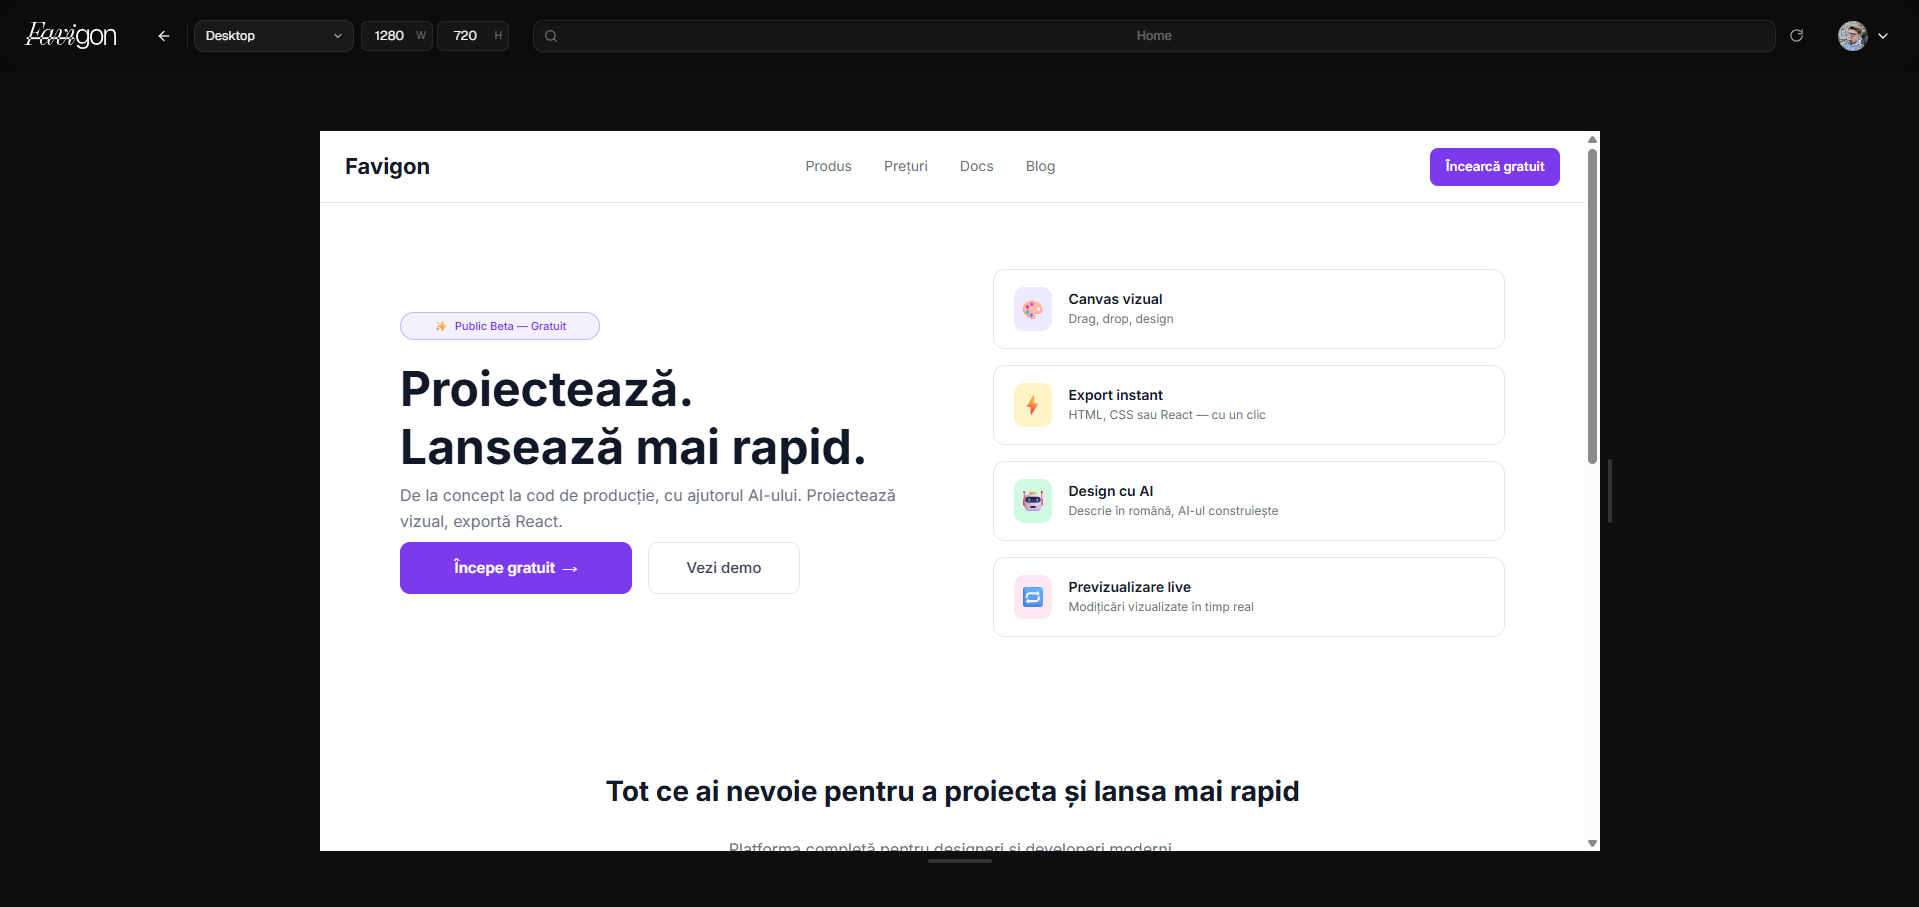
\includegraphics[width=0.96\textwidth]{images/project_preview.png}
  \caption{Pagina de preview folosită pentru vizualizarea rezultatului generat}
  \label{fig:project-preview}
\end{figure}

\subsection{Persistare și integrare cu restul aplicației}

Editorul nu este un spațiu închis. El comunică permanent cu serviciile de proiect, cu zona de preview și cu motorul de conversie. `CanvasPersistenceService` este legătura principală dintre starea editorului și backend. `CanvasGenerationService` este puntea spre export. `CanvasAiChatPersistenceService` și istoricul extind editorul dincolo de o simplă editare de suprafață.

Din punct de vedere practic, această integrare a fost mai grea decât scrierea unui editor minimal. Nu era suficientă mutarea unui element pe ecran; era necesară și posibilitatea de salvare, validare, export și reîncărcare a rezultatului fără inconsistențe majore.

\subsection{Persistența locală a conversației AI}

O extensie utilă a editorului este păstrarea locală a conversației AI și a contextului asociat. `CanvasAiChatPersistenceService` folosește `IndexedDB` pentru a salva, per proiect, mesajele recente, promptul aflat în lucru, modelul selectat și tab-ul activ al interfeței. Persistarea este făcută cu debounce de 300 ms, iar la restaurare sunt acceptate doar intrările mai noi de 7 zile. În plus, serviciul limitează mesajele păstrate la 40 și normalizează lungimea textelor, pentru a evita acumularea necontrolată de date în browser.

Această decizie completează bine autosave-ul clasic al designului. Documentul proiectului rămâne în backend, pentru a putea fi sincronizat și exportat, în timp ce conversația AI și contextul ei imediat rămân locale, ceea ce reduce trafic inutil și permite reluarea rapidă a sesiunii după reîncărcarea editorului. Împreună cu restaurarea istoricului și cu flush-ul la ieșire din pagină, rezultă un comportament mult mai apropiat de un instrument de lucru continuu decât de un simplu demo de generare.

\begin{figure}[H]
  \centering
  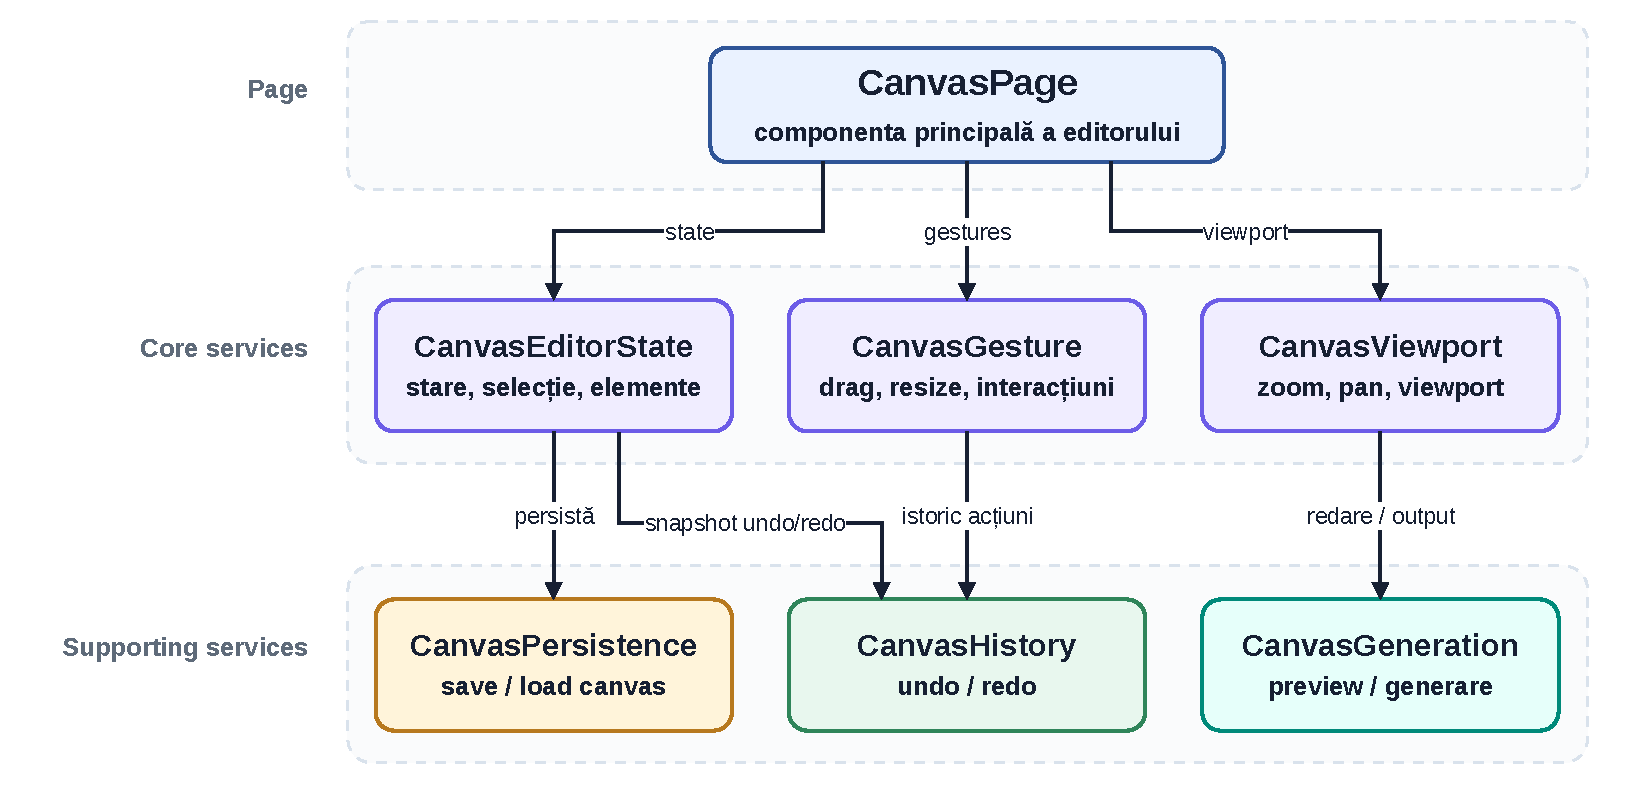
\includegraphics[width=0.96\textwidth]{diagrams/canvas-servicii.drawio.pdf}
  \caption{Servicii principale implicate în funcționarea editorului canvas}
  \label{fig:canvas-servicii}
\end{figure}

\section{Decizii de implementare cu impact major}

Privind la implementarea efectivă, există câteva decizii care au avut impact direct asupra stabilității și clarității codului.

Prima este faptul că logica specifică canvas-ului a fost păstrată în interiorul feature-ului `canvas`. În multe proiecte, utilitarele și serviciile migrează rapid spre zone generice, dar aici asta ar fi redus claritatea.

A doua este persistarea automată cu retry și flush controlat. Nu este o funcție spectaculoasă în demo, dar este foarte importantă în utilizare reală.

A treia este tratarea editorului ca pe o sumă de servicii coordonate, nu ca pe o singură componentă imensă care face totul. Deși `CanvasPage` rămâne o componentă mare, mare parte din comportament este împinsă în servicii.

A patra este integrarea atentă dintre proiecte, thumbnail-uri și asset-uri. Fără această zonă, editorul ar fi avut o viață scurtă în afara unei sesiuni locale.

\section{Concluzii intermediare}

Implementarea platformei arată că Favigon este mai mult decât un proof of concept pentru generare AI. Autentificarea, proiectele, profilurile, funcțiile sociale și editorul canvas formează împreună baza produsului. În această bază, editorul este modulul cel mai complex, dar el nu ar avea aceeași valoare fără restul infrastructurii de produs.

Capitolul următor tratează componenta care diferențiază cel mai mult proiectul din punct de vedere tehnic: generarea asistată de AI și conversia interfețelor în cod.

\chapter{Generarea asistată de AI și conversia interfețelor în cod}

\section{De ce nu este suficientă generarea directă}

Una dintre ideile tentante atunci când lucrezi cu modele generative este să ceri direct rezultatul final: ``generează-mi o pagină'' sau chiar ``generează-mi codul pentru această pagină''. Pentru demonstrații scurte, abordarea funcționează uneori surprinzător de bine. Totuși, pentru un produs software real, ea are câteva probleme serioase.

Prima problemă este controlul redus. Dacă modelul returnează direct cod, devine mai greu de separat unde s-a produs eroarea: în înțelegerea intenției, în structurarea layout-ului sau în alegerea stilurilor. A doua problemă este validarea. Codul poate arăta plauzibil fără să respecte constrângeri importante ale produsului. A treia problemă este reutilizarea. Dacă fiecare rezultat vine direct ca ieșire finală, nu există neapărat un nivel intern stabil pe care să îl poți edita și exporta în mai multe direcții.

Din aceste motive, în Favigon generarea asistată de AI este tratată ca un pipeline compus din etape distincte, nu ca pe un apel singular. În implementare, acest pipeline este orchestrat de `AiPipelineService`, iar integrarea cu modelul se face prin `OpenAiClient`.

\section{Principiul pipeline-ului în trei faze}

Soluția implementată în proiect împarte generarea în trei faze:

\begin{enumerate}[leftmargin=1.5cm]
  \item \textbf{intenție}: înțelegerea cererii și extragerea unei descrieri structurate a paginii;
  \item \textbf{structură}: construirea arborelui intermediar de noduri, layout-uri și dimensiuni;
  \item \textbf{stilizare}: aplicarea deciziilor vizuale pe structura deja generată.
\end{enumerate}

Această împărțire pare simplă, dar în practică aduce mai multe avantaje. Fiecare etapă are un contract mai clar. Fiecare etapă poate fi testată sau inspectată separat. Fiecare etapă poate fi oprită anticipat dacă utilizatorul vrea doar o schiță. În plus, dacă rezultatul unei etape este invalid, eroarea este mai ușor de localizat. Fluxul general al acestei orchestrări este sintetizat în Figura~\ref{fig:pipeline-ai}.

\begin{figure}[H]
  \centering
  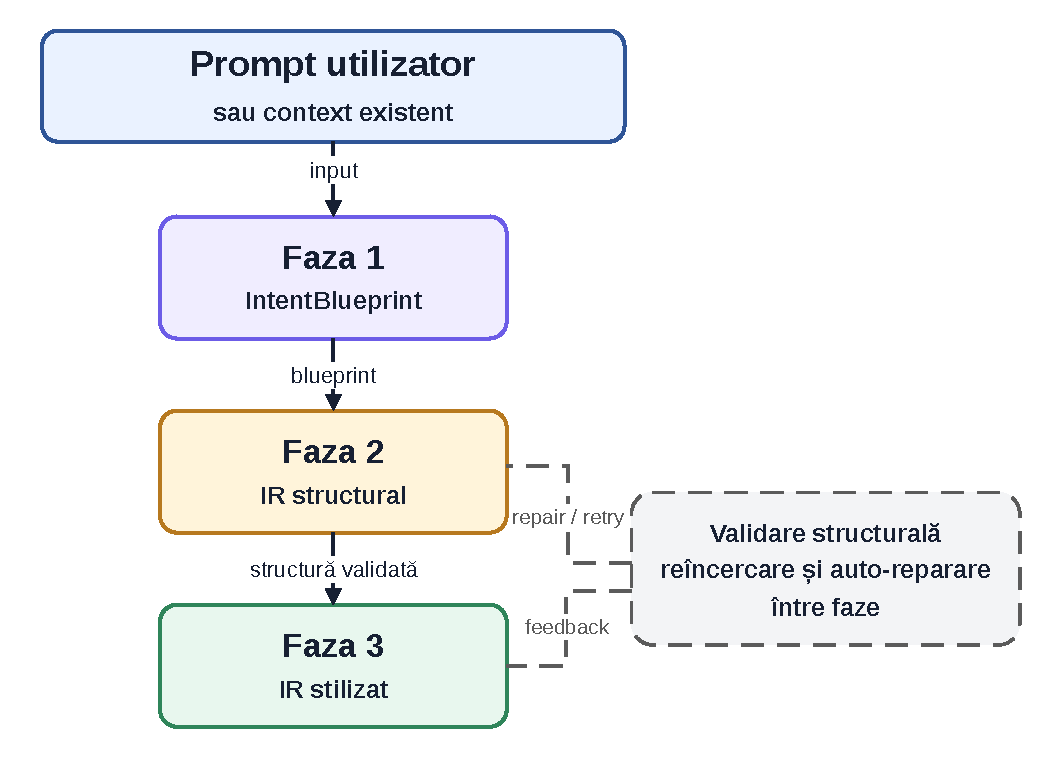
\includegraphics[width=0.80\textwidth]{diagrams/pipeline-ai.drawio.pdf}
  \caption{Pipeline-ul AI în trei faze folosit în Favigon}
  \label{fig:pipeline-ai}
\end{figure}

\section{Faza 1: extragerea intenției}

În prima etapă, sistemul nu încearcă să deseneze nimic și nu generează cod. Obiectivul este mai restrâns: să transforme promptul utilizatorului într-un \textit{IntentBlueprint}. În implementare, acest blueprint conține informații precum tipul paginii, starea vizuală generală, personalitatea brandului, publicul țintă, CTA-ul principal și lista secțiunilor în ordinea lor.

Acest pas explicit este important din două motive. În primul rând, el forțează modelul să ia o decizie de structură înainte să intre în detalii estetice. În al doilea rând, oferă frontend-ului și backend-ului o reprezentare intermediară ușor de afișat, inspectat sau discutat.

În practică, această etapă seamănă mai mult cu o analiză de cerințe decât cu o generare vizuală. Promptul este reinterpretat într-un format intern. Dacă utilizatorul cere, de exemplu, o pagină de prezentare pentru un produs SaaS, rezultatul nu trebuie să fie imediat un hero cu gradient, ci o listă de secțiuni și intenții: navbar, hero, beneficii, social proof, CTA, footer și așa mai departe.

\section{Faza 2: generarea structurii}

A doua etapă este cea care construiește efectiv arborele intermediar de noduri și reprezintă etapa centrală a întregii abordări. În loc să fie cerute modelului HTML final sau componente de framework, sarcina transmisă este producerea unui arbore `IRNode` cu layout, dimensiuni, padding, gap, poziționare și text.

Mai concret, structura generată include tipuri de noduri, copii, meta-informații, stiluri și reguli de layout. Promptul sistem pentru această fază este mult mai strict decât în prima etapă și include reguli explicite despre cum trebuie dimensionate secțiunile, cum trebuie folosite tipografiile, ce înseamnă `fit-content`, când se poate folosi `100%` și cum trebuie numite nodurile.

Această rigiditate este intenționată. Dacă în faza de intenție modelul are libertate mai mare, în faza structurală libertatea trebuie redusă. Altfel, ar exista prea multe variații greu de validat și greu de convertit.

\section{Faza 3: stilizarea}

A treia etapă pornește de la structura deja creată și aplică sistemul vizual: culori, gradiente, umbre, raze, borduri, cursor și alte detalii de prezentare. În implementare, promptul pentru această fază conține o regulă foarte importantă: layout-ul și structura nu trebuie modificate. Altfel spus, stilizarea nu are voie să rescrie ceea ce a rezolvat deja etapa de structură.

Această separare între structură și stil este utilă atât pentru control, cât și pentru depanare. Dacă o pagină este logică, dar arată slab, știu că problema este în faza a treia. Dacă layout-ul este greșit, știu că problema este în faza a doua. În plus, această abordare seamănă mai bine cu modul în care lucrează și oamenii: întâi decid structura și ierarhia, apoi rafinează aspectul vizual.

\section{Integrarea cu OpenAI API}

În Favigon, comunicarea cu modelul este abstractizată prin `OpenAiClient`. Acesta folosește endpoint-ul de \textit{Chat Completions} și suportă atât răspuns obișnuit, cât și streaming \cite{openaiChatCompletions2026}. Alegerea de a ascunde apelurile HTTP într-un adaptor de infrastructură păstrează serviciile de aplicație concentrate pe logică și face mai ușoară înlocuirea sau extinderea integrării în viitor.

Clientul construiește payload-ul cu mesaj de sistem, mesaj de utilizator, model configurabil și, unde este cazul, \texttt{response\_format} bazat pe schemă JSON. În plus, pentru scenariile de streaming, clientul parcurge liniile SSE și extrage incremental conținutul transmis de model. În implementarea actuală, identificatorul modelului este citit din configurație, cu fallback la \texttt{gpt-5.4-mini}, iar cererile trimit atât \texttt{response\_format}, cât și un prag explicit de \texttt{max\_completion\_tokens} pentru a limita comportamentul apelului la parametri observați și reproductibili.

Păstrarea identificatorului modelului în configurație, nu hardcodat în logică, este importantă deoarece partea experimentală a aplicației poate necesita ajustări de model în timp, iar aceste schimbări nu ar trebui să implice recompilarea serviciului de aplicație.

\section{Structura cererilor AI și feedback incremental}

Din punctul de vedere al API-ului, integrarea AI nu primește doar un simplu șir de text. Cererea de bază către endpoint-urile de design include promptul, un viewport țintă, modelul ales și, opțional, o structură IR existentă. Acest ultim câmp este important deoarece permite scenarii în care utilizatorul nu cere generarea unei pagini de la zero, ci rafinarea sau extinderea unei structuri deja existente. În cazul pipeline-ului pe trei faze, aceeași cerere mai include și parametrul \texttt{StopAfterPhase}, ceea ce face posibilă oprirea controlată după faza de intenție sau după faza structurală.

\begin{table}[H]
  \centering
  \caption{Câmpuri relevante din cererile AI folosite de backend}
  \label{tab:campuri-cereri-ai}
  \renewcommand{\arraystretch}{1.15}
  \begin{tabularx}{\textwidth}{>{\RaggedRight\arraybackslash}p{3.2cm}YY}
    \toprule
    \textbf{Câmp} & \textbf{Semnificație} & \textbf{Rol în procesare} \\
    \midrule
    \texttt{Prompt} & descrierea textuală a interfeței dorite & punctul de pornire pentru interpretarea intenției \\
    \texttt{ExistingIr} & structură intermediară existentă, opțională & permite extindere, reparare sau rafinare în loc de generare complet nouă \\
    \texttt{ViewportWidth} & lățimea de referință a paginii generate & influențează presupunerile de layout și scară \\
    \texttt{Model} & identificatorul modelului folosit & permite alegerea explicită între variantele configurate \\
    \texttt{StopAfterPhase} & limită de oprire pentru pipeline-ul în 3 faze & utilă pentru schițe parțiale, depanare și observarea etapelor intermediare \\
    \bottomrule
  \end{tabularx}
\end{table}

Suportul pentru streaming schimbă semnificativ și experiența utilizatorului. În loc să aștepte un singur răspuns final, frontend-ul poate primi evenimente incremental și poate afișa progresul procesării. În implementarea actuală, endpoint-urile de streaming trimit răspunsuri de tip \texttt{text/event-stream}, iar backend-ul emite linii SSE în care tipul evenimentului și conținutul sunt transmise separat. Pentru pipeline-ul în trei faze, evenimente precum \texttt{phase\_start}, \texttt{phase\_complete}, \texttt{result} sau \texttt{error} oferă o vizibilitate mult mai bună asupra procesului decât o simplă animație de încărcare.

\begin{lstlisting}[style=favigon,caption={Exemplu simplificat de evenimente SSE trimise în timpul pipeline-ului AI}]
event: phase_start
data: {"phase":1,"name":"intent"}

event: phase_complete
data: {"phase":1,"name":"intent"}

event: result
data: {"success":true,"stopAfterPhase":3}
\end{lstlisting}

Din punct de vedere operațional, fluxul complet dintre utilizator, frontend, controller, orchestration service și modelul AI este mai bine surprins printr-o diagramă de secvență. Figura~\ref{fig:secventa-ai} evidențiază atât schimburile principale de mesaje, cât și faptul că pipeline-ul nu este un singur apel, ci o succesiune controlată de faze cu feedback incremental.

\begin{figure}[H]
  \centering
  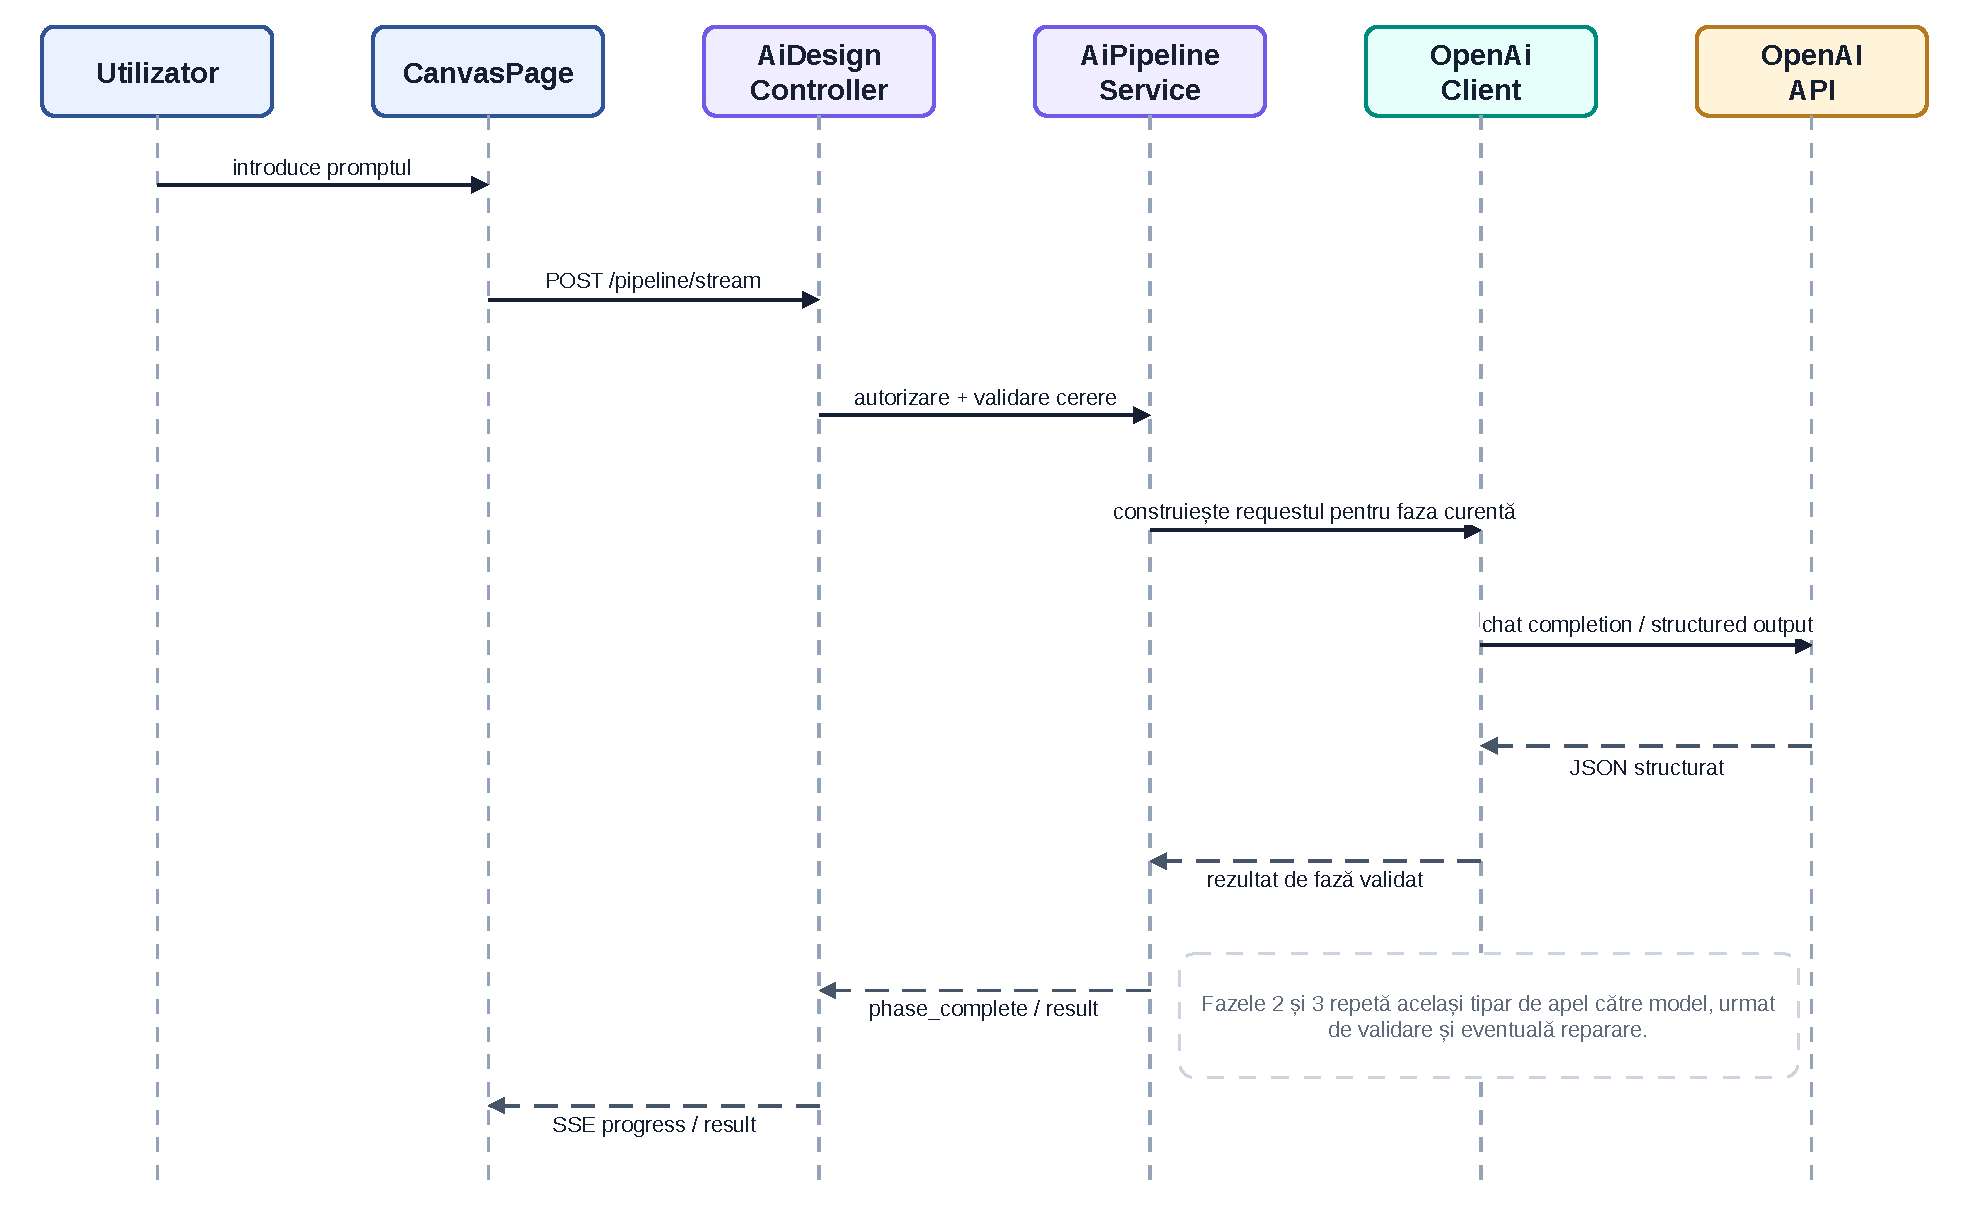
\includegraphics[width=\textwidth]{diagrams/secventa-ai.drawio.pdf}
  \caption{Diagrama de secvență simplificată pentru fluxul AI cu streaming}
  \label{fig:secventa-ai}
\end{figure}

\section{Rolul ieșirilor structurate}

OpenAI documentează explicit posibilitatea obținerii unor ieșiri structurate, conforme cu un anumit format sau cu o anumită schemă \cite{openaiStructuredOutputs2026}. În proiect, această capabilitate este foarte importantă. Dacă modelul ar întoarce doar text liber, parser-ul și validarea ar deveni mult mai fragile. În schimb, cu o schemă bine definită, aplicația poate detecta mai repede abaterile și poate decide dacă rezultatul este utilizabil sau nu.

Totuși, experiența din implementare arată că \textit{structured output} nu este o soluție magică. El ajută la format, dar nu garantează automat calitatea semantică a rezultatului. De exemplu, un JSON perfect valid poate descrie o structură slabă sau o ierarhie de secțiuni nepotrivită. Din acest motiv, `AiPipelineService` folosește atât deserializare și validare structurală, cât și reguli suplimentare și un pas de auto-reparare când rezultatul nu este acceptabil.

\section{Mecanisme de validare și reparare}

După fiecare etapă relevantă, rezultatul este analizat înainte să fie acceptat. Dacă în faza structurală arborele IR nu poate fi parsat sau nu respectă schema așteptată, serviciul încearcă un pas suplimentar de reparare. Acest pas trimite către model erorile de validare și o variantă trunchiată a rezultatului defect, cerând un JSON corectat.

Practic, modelul este tratat nu doar ca generator, ci și ca potențial asistent pentru repararea propriilor ieșiri. Această idee este utilă în contextul lucrării deoarece arată un mod mai realist de folosire a AI-ului: prima ieșire nu este presupusă perfectă, iar sistemul este proiectat explicit pentru a gestiona erori.

În plus, atât `AiDesignService`, cât și `AiPipelineService` folosesc cache cu TTL de 10 minute pentru cereri identice și validează separat răspunsurile obținute. În varianta de pipeline există și posibilitatea de oprire după faza 1 sau 2, respectiv emiterea de evenimente SSE de tip \texttt{phase\_start} și \texttt{phase\_complete}, ceea ce face procesul mai ușor de urmărit în interfață și în depanare.

\section{Reprezentarea intermediară în detaliu}

Structura `IRNode` este elementul care leagă editorul, AI-ul și convertorul. Un nod include identificator, tip, proprietăți, layout, stil, poziționare, copii, variante responsive, metadate și, opțional, efecte de animație. Această structură este suficient de generală pentru a descrie atât containere, cât și text, imagini sau frame-uri de pagină.

În practică, modelul intermediar oferă trei beneficii majore.

Primul este \textbf{independența față de framework}. Un `IRNode` nu este nici componentă Angular, nici JSX React, nici HTML final. De aceea poate fi transformat în toate aceste forme.

Al doilea este \textbf{validabilitatea}. Pentru că structura este explicită, poate fi verificată existența anumitor câmpuri, coerența layout-ului sau compatibilitatea dimensiunilor înainte de export.

Al treilea este \textbf{trasabilitatea}. Când ceva nu merge bine în export, structura intermediară poate fi inspectată și se poate vedea dacă problema vine din editor, din AI sau din convertor.

\section{Maparea dintre canvas și IR}

Pe partea de frontend, designul construit în editor nu este trimis direct către convertor în forma nativă a canvas-ului. În schimb, există mapper-e care transformă datele editorului în IR și invers. Acest detaliu este foarte important pentru arhitectura proiectului.

Dacă editorul ar fi legat direct de codul final, orice schimbare în convertor ar risca să rupă și logica din canvas. Prin introducerea mapper-elor, este creat un punct de decuplare. Editorul poate evolua într-o anumită direcție, iar convertorul în alta, atâta timp cât contractul IR rămâne coerent.

Maparea inversă, din IR în elemente de canvas, este la fel de utilă. Ea face posibilă integrarea rezultatelor generate de AI direct în editor, astfel încât utilizatorul să nu primească un export static, ci un design pe care îl poate modifica în continuare.

\section{Exemplu concret de flux de la prompt la IR și export}

Pentru a înțelege mai clar legătura dintre subsisteme, este util un exemplu simplificat. Presupunând un prompt de tipul „creează o pagină landing pentru o aplicație de task management, cu hero, beneficii și call-to-action”, prima fază nu produce HTML și nici noduri finale, ci o descriere structurată a intenției: tip de pagină, audiență, ton vizual și secțiuni în ordinea așteptată. A doua fază transformă această intenție într-un arbore IR cu frame principal, containere, text și butoane, iar a treia aplică stilurile. Abia după aceste etape structura ajunge la convertor.

În etapa de export, convertorul primește fie un singur \texttt{IRNode}, fie o listă de pagini. Pentru cazul simplu single-page, \texttt{ConverterController} apelează validarea și apoi \texttt{Generate}. Pentru cazul multi-page, aceeași rută de generare poate primi \texttt{Pages}, iar endpoint-ul dedicat pentru fișiere folosește \texttt{GenerateMultiPage}. Rezultatul nu este doar o bucată de cod brut, ci un set coerent de artefacte adaptate framework-ului cerut: HTML și CSS pentru varianta statică, respectiv fișiere de componentă, stil și structură pentru React sau Angular.

Acest exemplu arată de ce separarea pe etape este importantă. Dacă problema apare în secționarea paginii sau în ierarhia elementelor, ea poate fi localizată înainte de convertor. Dacă structura este corectă, dar codul rezultat nu respectă așteptările, zona de investigație se mută în motorul de export. În practică, această trasabilitate reduce mult costul depanării și face sistemul mai explicabil în comparație cu o abordare directă „prompt în, cod afară”.

\section{Motorul de conversie}

\subsection{Separarea în proiect dedicat}

Motorul de conversie este implementat în proiectul `Favigon.Converter`. El este separat explicit de `Favigon.Application` deoarece are propria logică de validare, transformare și emitere. Dacă ar fi rămas îngropat în același serviciu cu restul aplicației, ar fi fost mai greu de testat și mai greu de extins.

\subsection{Validarea}

Înainte de generare, `ConverterService` cere motorului verificarea structurii IR. Dacă apar erori, ele sunt raportate și procesul se oprește. Această etapă este necesară pentru că ieșirea finală ar deveni altfel imprevizibilă. Este preferabil refuzul unui export decât generarea de cod inconsistent fără semnalarea problemei.

\subsection{Generarea single-page și multi-page}

`ConverterEngine` suportă atât generarea pentru o singură pagină, cât și generarea pentru mai multe pagini. Pentru multi-page, motorul produce seturi de fișiere și gestionează numele de pagini, slug-urile și structura finală. În cazul exportului Angular sau React, el generează și fișiere de proiect minimal, rute și fișiere CSS.

Această capabilitate este importantă deoarece proiectul nu se reduce la o singură artboard. Odată ce editorul suportă mai multe pagini, exportul trebuie să poată păstra această structură.

\begin{figure}[H]
  \centering
  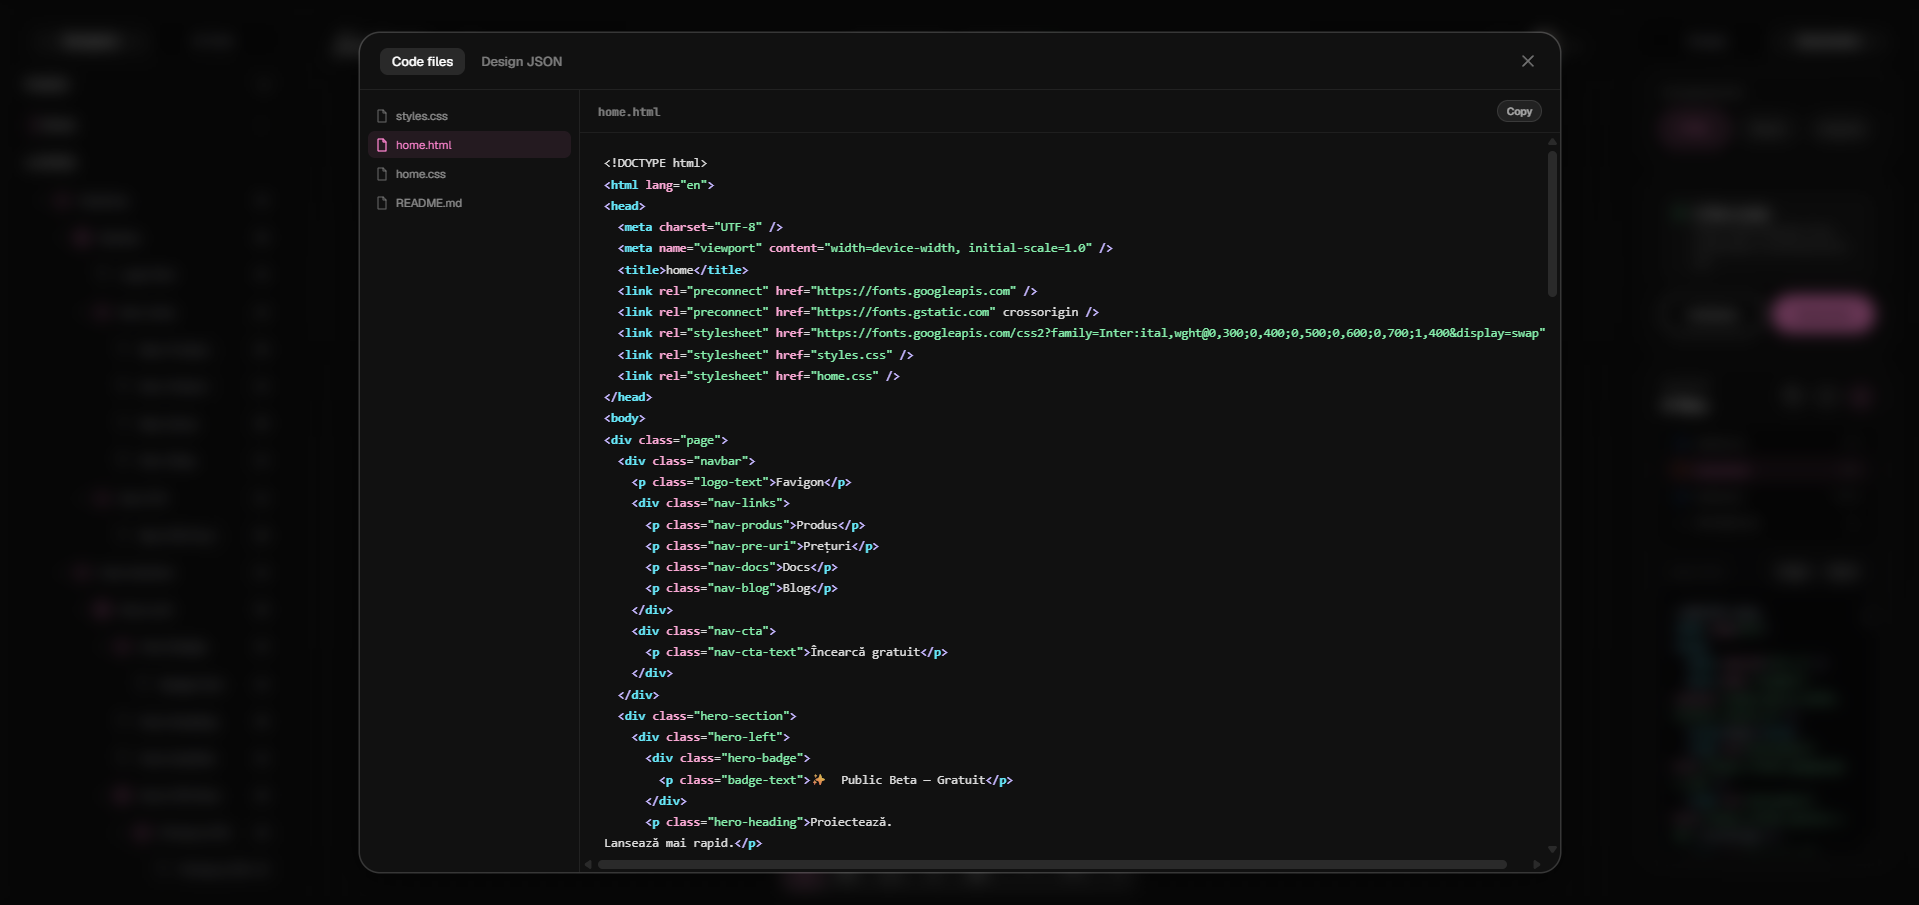
\includegraphics[width=0.94\textwidth]{images/generated_code.png}
  \caption{Exemplu de artefacte generate și inspectate în interfața de export}
  \label{fig:generated-code}
\end{figure}

\subsection{Responsive output}

O componentă mai tehnică și mai interesantă este exportul responsive. În loc să dublez pur și simplu tot arborele pentru fiecare breakpoint, motorul produce artefactele principale și apoi diferențe CSS pentru breakpoints suplimentare. În testele existente se vede că sunt tratate cazuri precum noduri prezente doar pe anumite breakpoint-uri, schimbări de ordine pentru copii flex și diferențe de pseudo-clase sau keyframes.

Aceasta este una dintre funcțiile care arată cel mai clar că proiectul nu se oprește la un export superficial. Există o preocupare reală pentru cum este construit rezultatul final și pentru cât de mult poate fi controlat. Fluxul complet canvas $\rightarrow$ IR $\rightarrow$ artefacte de export este rezumat în Figura~\ref{fig:design-to-code}.

\begin{figure}[H]
  \centering
  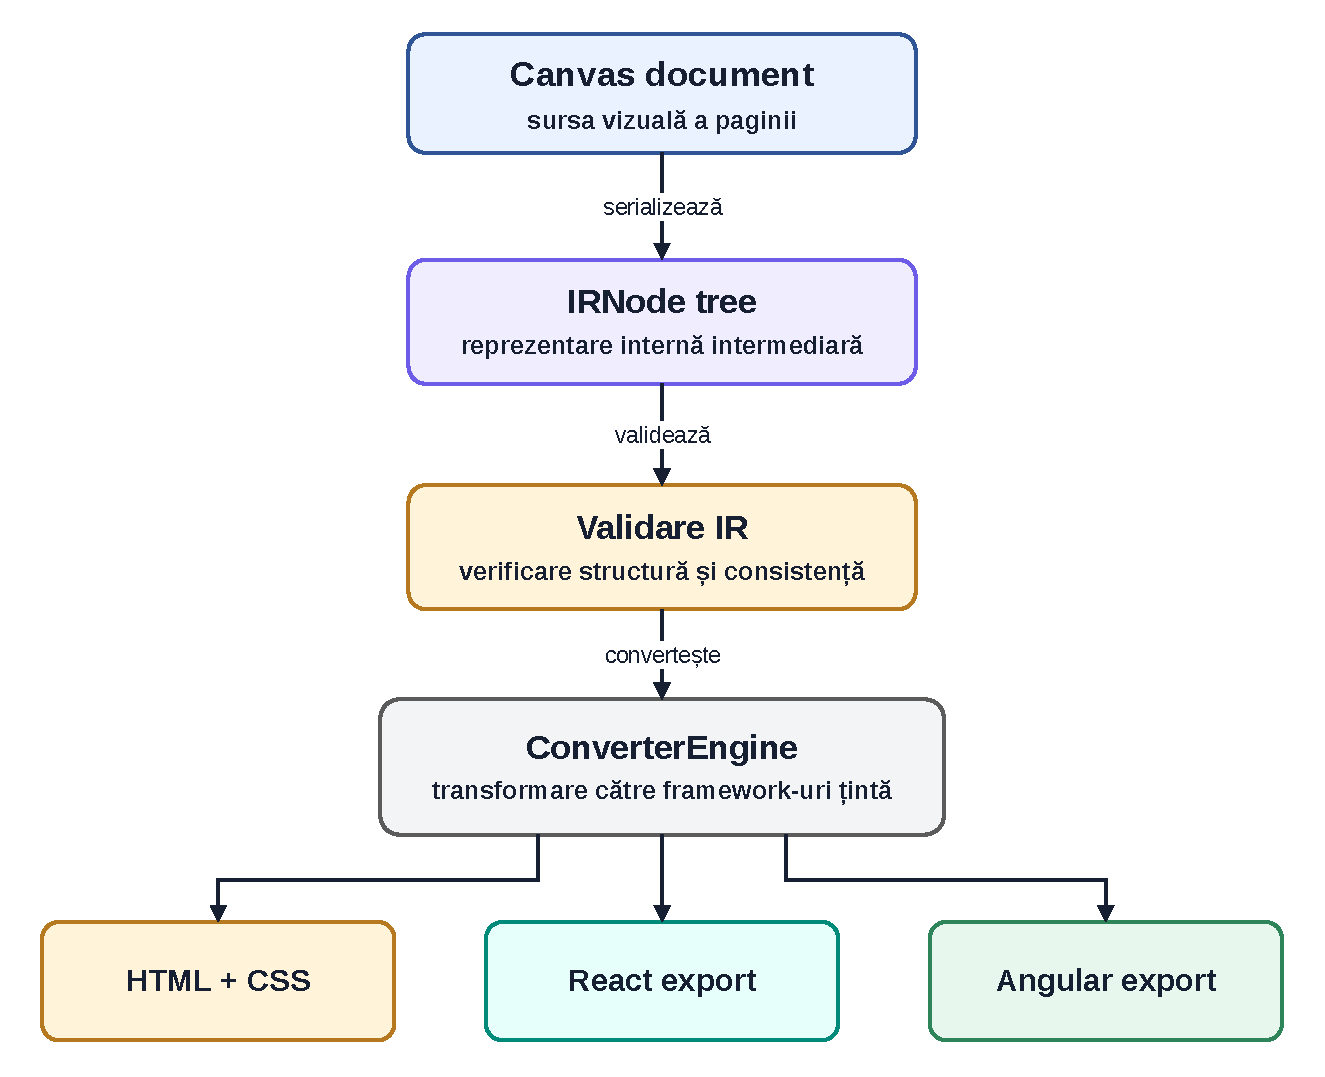
\includegraphics[width=0.90\textwidth]{diagrams/design-to-code.drawio.pdf}
  \caption{Fluxul design-to-code bazat pe reprezentarea intermediară}
  \label{fig:design-to-code}
\end{figure}

\section{Legătura dintre AI și convertor}

Un aspect foarte important este faptul că AI-ul și convertorul nu sunt două subsisteme complet separate. Ele comunică prin aceeași reprezentare intermediară. Fără această alegere, rezultatul generat de AI ar fi fost mult mai greu de transformat în cod într-un mod controlat.

Pe scurt, pipeline-ul AI generează un arbore care este suficient de bogat pentru a fi editat și suficient de formal pentru a fi convertit. În momentul în care această condiție este îndeplinită, editorul devine interfața de rafinare, iar convertorul devine ieșirea tehnică. Această relație dintre cele trei module --- AI, editor și convertor --- reprezintă contribuția tehnică principală a întregului proiect.

\section{Limitări actuale}

Deși soluția funcționează și este coerentă, există și limite.

În primul rând, calitatea rezultatului AI depinde încă mult de prompt și de regulile incluse în mesajele de sistem. Cu alte cuvinte, caracterul probabilistic al modelului nu este eliminat; el este doar controlat mai bine.

În al doilea rând, reprezentarea intermediară este suficient de bogată pentru scopurile actuale, dar nu acoperă toate situațiile pe care le-ar avea un constructor comercial matur. De exemplu, colaborarea în timp real, constrângerile mai avansate de componentizare sau integrarea automată cu design systems externe ar necesita extinderi suplimentare.

În al treilea rând, exportul generat este orientat spre claritate și portabilitate, nu neapărat spre cele mai sofisticate convenții ale fiecărui ecosistem. Pentru o platformă academică, acest compromis este acceptabil.

\section{Concluzii intermediare}

Capitolul de față descrie partea cea mai originală din proiect. Generarea asistată de AI nu este tratată ca un artificiu separat, ci ca parte a unei arhitecturi care include reprezentare intermediară, validare, reparare și conversie în cod. Tocmai această integrare controlată face diferența între o demonstrație izolată și un produs software coerent.

În capitolul următor sunt urmărite scenarii concrete de utilizare, pentru a observa cum colaborează în practică editorul, AI-ul, preview-ul, exportul și componenta socială. Abia după această etapă este discutată explicit validarea sistemului prin măsuri de securitate și testare.



\chapter{Scenarii de utilizare și evaluare practică}

\section{Rolul acestui capitol în contextul lucrării}

După prezentarea arhitecturii, a implementării și a mecanismelor de generare asistată de AI, este utilă o etapă intermediară în care aplicația să fie privită ca produs utilizabil, nu doar ca ansamblu de module. În practică, valoarea unui sistem precum Favigon nu rezultă numai din existența unui editor canvas, a unui pipeline AI sau a unui convertor, ci din felul în care acestea lucrează împreună într-un flux coerent pentru utilizator.

Din acest motiv, capitolul de față urmărește câteva scenarii reprezentative, alese astfel încât să acopere atât utilizarea clasică a editorului, cât și scenariile care implică generare asistată, publicare și reutilizare. Scopul nu este repetarea implementării descrise deja în capitolele anterioare, ci observarea modului în care subsistemele colaboratoare se comportă atunci când sunt folosite cap-coadă.

În plus, această abordare ajută și la justificarea deciziilor de proiectare. Unele alegeri care par excesiv de tehnice atunci când sunt privite izolat, de exemplu reprezentarea intermediară, persistarea automată sau separarea convertorului într-un proiect dedicat, devin mai ușor de înțeles când sunt raportate la pașii parcurși de utilizator într-un scenariu concret.

\section{Criteriile urmărite în evaluarea practică}

Scenariile alese nu urmăresc performanțe de benchmark și nici o comparație formală cu produse comerciale. Ele au un obiectiv mai simplu și mai potrivit pentru lucrarea de față: să arate dacă fluxurile importante ale produsului pot fi parcurse fără rupturi majore între editare, persistare, generare, preview, export și publicare.

La nivel concret, au fost urmărite patru criterii.

\begin{enumerate}[leftmargin=1.5cm]
  \item \textbf{coerența fluxului de lucru}, adică măsura în care utilizatorul poate trece natural de la o etapă la alta;
  \item \textbf{trasabilitatea rezultatului}, adică posibilitatea de a înțelege de unde provine un anumit rezultat și în ce zonă apare o problemă;
  \item \textbf{stabilitatea operațiilor frecvente}, precum salvarea, schimbarea paginilor, preview-ul și exportul;
  \item \textbf{continuitatea dintre zona de creație și zona socială}, adică publicarea, explorarea și reutilizarea proiectelor.
\end{enumerate}

Aceste criterii au fost alese deoarece reflectă direct obiectivele proiectului. Favigon nu își propune doar să deseneze elemente pe un canvas și nici doar să apeleze un model AI, ci să ofere un traseu relativ complet de la idee la rezultat reutilizabil. În consecință, o evaluare practică relevantă trebuie să urmărească exact această continuitate.

\section{Scenariul 1: creare manuală și export al unui proiect}

Primul scenariu urmărește utilizarea aplicației fără generare AI, pentru a observa în ce măsură editorul, persistarea și exportul pot susține singure fluxul principal de lucru. Scenariul pornește de la crearea unui proiect nou și continuă cu editarea lui în canvas, verificarea prin preview și obținerea artefactelor finale de export.

În practică, utilizatorul începe prin crearea unui proiect și deschiderea editorului dedicat. Odată încărcată pagina, interfața principală a editorului oferă atât zona de lucru, cât și panourile laterale necesare pentru navigarea printre pagini, inspectarea structurii și modificarea proprietăților. Figura~\ref{fig:canvas-editor} ilustrează această stare de lucru și este relevantă deoarece arată că editorul nu este tratat ca o simplă suprafață grafică, ci ca un spațiu în care structura documentului și proprietățile elementelor rămân vizibile și controlabile.

În acest scenariu, utilizatorul construiește manual o pagină de prezentare simplă, formată dintr-un navbar, o secțiune hero, o zonă de beneficii și un call-to-action final. Din perspectiva experienței de lucru, un aspect important este faptul că operațiile de selecție, mutare, redimensionare și configurare a proprietăților sunt integrate într-un singur flux. Utilizatorul nu lucrează separat într-un ``mod de design'' și într-un ``mod de structură'', ci vede în același timp atât rezultatul vizual, cât și organizarea internă a elementelor.

Această observație este importantă pentru că arată rolul serviciilor descrise în capitolul precedent. `CanvasEditorStateService`, `CanvasGestureService` și `CanvasViewportService` nu apar direct în interfață sub forma unor concepte teoretice, dar efectul lor cumulat devine vizibil tocmai în astfel de operații simple. Dacă ele nu ar colabora corect, editorul ar părea imediat inconsistent: selecția ar rămâne în urmă, gesturile ar reacționa prost sau starea documentului s-ar rupe de suprafața vizuală.

Un al doilea aspect urmărit în acest scenariu este persistarea. În timpul editării, modificările nu sunt gândite ca acțiuni care trebuie confirmate permanent de utilizator prin salvare manuală. În schimb, editorul folosește autosave cu debounce și flush controlat la ieșirea din pagină. Din punct de vedere practic, această alegere este foarte importantă. Într-un produs de tip design tool, orice dependență excesivă de salvare manuală ar rupe ritmul de lucru și ar transforma editorul într-un prototip fragil.

În cazul Favigon, comportamentul observat este apropiat de cel așteptat pentru un instrument de lucru continuu. Utilizatorul poate face mai multe modificări succesive, poate schimba selecția, poate naviga între pagini și poate reveni asupra unor elemente fără să aibă impresia că lucrează împotriva mecanismului de persistență. Acest lucru nu elimină toate riscurile, dar arată că partea de autosave nu a rămas un detaliu de implementare, ci susține direct experiența de utilizare.

După editare, scenariul continuă cu verificarea rezultatului în pagina de preview. Aici apare una dintre diferențele importante dintre suprafața de editare și produsul rezultat. În locul reproducerii directe a documentului intern al editorului, aplicația reconstruiește reprezentarea intermediară și cere backend-ului generarea HTML/CSS pentru pagina curentă. Figura~\ref{fig:project-preview} arată această etapă și evidențiază faptul că preview-ul funcționează ca un pas de validare realistă, nu ca o simplă captură a canvas-ului.

Din punct de vedere practic, preview-ul este util din două motive. Primul este validarea vizuală: utilizatorul poate observa mai ușor cum arată rezultatul într-un mediu mai apropiat de randarea finală. Al doilea este validarea fluxului tehnic: dacă designul arată corect în editor, dar nu se mai păstrează în preview, problema nu mai este în zona de manipulare vizuală, ci în maparea către IR sau în convertor.

Ultimul pas al scenariului este exportul. Odată ce pagina a fost verificată, utilizatorul poate cere generarea artefactelor finale. Figura~\ref{fig:generated-code} ilustrează o astfel de situație și arată că ieșirea nu constă într-un singur bloc de text, ci într-un set de fișiere inspectabile. Pentru lucrarea de față, acest detaliu este important deoarece arată că fluxul nu se oprește la o promisiune de tip ``design-to-code'', ci duce efectiv la un rezultat care poate fi citit și reutilizat.

Per ansamblu, acest prim scenariu confirmă că Favigon poate susține un traseu complet chiar și fără AI: creare, editare, salvare, preview și export. Asta este relevant deoarece demonstrează că aplicația nu depinde complet de componenta generativă pentru a avea sens ca produs. AI-ul extinde sistemul, dar nu îl înlocuiește.

\section{Scenariul 2: generare pornind de la prompt și rafinare ulterioară}

Al doilea scenariu urmărește zona care diferențiază cel mai mult proiectul: utilizarea AI-ului ca punct de pornire pentru construcția unei interfețe, urmată de integrarea rezultatului în editor și de rafinarea lui manuală. Acest scenariu este important pentru că arată dacă relația dintre prompt, pipeline, reprezentare intermediară și editare directă rămâne coerentă și în practică, nu doar la nivel conceptual.

Punctul de pornire este un prompt de nivel produs, de exemplu o cerere pentru o pagină landing a unei aplicații SaaS, cu secțiuni standard, accent pe call-to-action și stil vizual modern. În această etapă, utilizatorul nu descrie fiecare pixel și nici nu dictează structura exactă a arborelui intern. Rolul promptului este să exprime intenția, iar sistemul trebuie să o transforme într-o bază de lucru utilizabilă.

Din punct de vedere arhitectural, acesta este exact contextul în care devine vizibil avantajul pipeline-ului în trei faze. Dacă generarea ar produce direct cod final, orice neclaritate din rezultat ar fi greu de localizat. În schimb, în Favigon, drumul trece prin intenție, structură și stilizare. Asta face ca rezultatul final să poată fi discutat și corectat pe etape. Chiar dacă utilizatorul final nu vede explicit fiecare structură intermediară, efectul este unul important: sistemul oferă un rezultat mai controlabil.

După finalizarea pipeline-ului, rezultatul nu rămâne izolat într-o fereastră de răspuns și nici nu este oferit doar ca export static. El este integrat în editor, unde poate fi tratat ca document de lucru normal. Din perspectiva produsului, acesta este probabil cel mai important pas al întregii aplicații. Dacă designul generat nu ar putea fi preluat în editor, Favigon ar rămâne mai aproape de un generator de mockup-uri decât de o platformă de design asistat.

Odată încărcat în editor, utilizatorul poate modifica structura, poate rescrie texte, poate ajusta dimensiuni, spațieri, culori și layout-uri, sau poate adăuga elemente noi. În acest fel, AI-ul funcționează ca accelerator al primei versiuni, nu ca autor final incontestabil al interfeței. Acest aspect este important și pentru tonul academic al lucrării, deoarece arată o abordare realistă: modelul propune o soluție inițială, iar utilizatorul rămâne în controlul rezultatului.

În practică, etapa de rafinare este cea care validează calitatea integrării dintre generare și editare. Dacă rezultatul AI ar intra în editor într-o formă greu de manipulat, cu elemente poziționate arbitrar sau cu proprietăți incoerente, întreaga idee de continuitate s-ar pierde. Observația importantă aici este că reprezentarea intermediară acționează tocmai ca stratul care face posibilă această tranziție. Designul generat poate fi tratat în același limbaj intern ca un design creat manual, ceea ce simplifică atât editarea, cât și exportul ulterior.

În plus, scenariul acesta evidențiază și una dintre limitările reale ale aplicației. Calitatea rezultatului inițial depinde încă de prompt și de disciplina regulilor folosite în mesajele de sistem. Uneori, prima variantă este foarte aproape de ce se dorește; alteori, ea cere ajustări mai vizibile. Totuși, tocmai faptul că rezultatul poate fi corectat în editor fără ruperea fluxului face ca această limitare să fie mai ușor de acceptat în practică.

După rafinare, utilizatorul poate relua pașii de preview și export, ca în scenariul anterior. Din această perspectivă, scenariul 2 nu este complet diferit de scenariul 1, ci îl extinde. Diferența este că punctul de intrare nu mai este o pagină goală, ci o propunere generată. În rest, traseul rămâne același: document editabil, preview realist și artefacte de ieșire inspectabile.

Acesta este un rezultat important pentru lucrare, deoarece arată că AI-ul nu introduce un ``tunel'' paralel în aplicație. El alimentează același flux general de produs. Din punct de vedere al proiectării software, aceasta este una dintre cele mai solide justificări pentru separarea dintre generare, reprezentare intermediară și conversie.

\section{Scenariul 3: publicare, explorare și reutilizare prin fork}

Al treilea scenariu urmărește trecerea din zona individuală de lucru în zona socială a aplicației. Pentru multe proiecte academice, această parte ar putea părea secundară, însă în cazul Favigon ea are un rol important: arată că rezultatele create nu rămân blocate în spațiul privat al unui singur utilizator, ci pot circula, pot fi descoperite și pot deveni puncte de plecare pentru alte proiecte.

Scenariul pornește de la un proiect considerat suficient de matur pentru a fi făcut public. După publicare, el devine eligibil pentru afișare în zona `Explore`, unde utilizatorii pot vedea proiecte populare sau recomandate și pot descoperi alți autori. Figura~\ref{fig:explore-page} este relevantă tocmai pentru această etapă, deoarece arată că aplicația nu se oprește la o listă administrativă de proiecte, ci oferă un spațiu distinct de descoperire.

Din punct de vedere al produsului, publicarea schimbă statutul proiectului. El nu mai este doar un document persistat în contul unui autor, ci o resursă care poate primi vizualizări, aprecieri și bookmark-uri și care poate fi asociată mai clar cu identitatea creatorului său. Acest lucru contează deoarece mută aplicația din zona unui instrument de lucru local către zona unui ecosistem mic, dar coerent, de creare și reutilizare.

O funcție deosebit de relevantă în acest context este fork-ul. Dacă un utilizator găsește un proiect public interesant, el poate crea o copie proprie pornind de la acel punct. Din perspectivă tehnică, această operație nu înseamnă doar duplicarea unui document JSON, ci păstrarea unei relații între proiectul-sursă și cel derivat. Din perspectivă practică, rezultatul este foarte util: reutilizarea devine concretă și trasabilă.

Acest scenariu este valoros și pentru că arată întâlnirea dintre două zone care altfel ar putea rămâne separate: partea de producție și partea socială. În multe produse, zona de explorare este doar un catalog de exemple. În Favigon, ea are efect direct asupra procesului de creație, deoarece un proiect descoperit public poate fi transformat într-un punct de pornire pentru o nouă iterație de editare și export.

Mai mult, acest scenariu oferă și un argument bun pentru existența infrastructurii de profiluri, follow, like, star și proiecte publice. Dacă lucrarea s-ar opri doar la generarea AI și la export, aceste funcții ar părea poate suplimentare. Însă, puse într-un flux concret de publicare, explorare și fork, ele capătă o justificare clară la nivel de produs.

\section{Observații asupra comportamentului sistemului}

Scenariile anterioare permit câteva observații generale despre comportamentul aplicației în utilizare practică.

Prima observație este că separarea pe subsisteme nu rupe experiența utilizatorului. Deși intern există granițe clare între editor, pipeline AI, convertor, backend REST și componenta socială, în utilizare acestea apar ca părți ale aceluiași produs. Acesta este un semn bun pentru proiect, fiindcă o arhitectură curată, dar resimțită de utilizator ca fragmentare, nu ar reprezenta un rezultat reușit.

A doua observație este că reprezentarea intermediară nu este doar o decizie tehnică elegantă, ci un element cu efect vizibil în flux. Ea face posibilă trecerea dintre editare, generare și export fără schimbarea ``limbajului intern'' al documentului. Din acest motiv, multe dintre operațiile discutate în scenariile anterioare par mai naturale decât ar părea într-un sistem bazat doar pe transformări ad-hoc între formate incompatibile.

A treia observație este că preview-ul joacă un rol mai important decât ar putea părea inițial. El nu este doar o etapă de prezentare, ci și un punct de control între documentul editabil și ieșirea finală. În practică, el ajută la separarea problemelor vizuale de problemele de conversie și reduce riscul ca utilizatorul să descopere abia la export că rezultatul nu corespunde așteptărilor.

A patra observație privește limitările rămase. Deși fluxul general este coerent, sistemul nu elimină complet costul rafinării manuale, mai ales în scenariile pornite din prompt. Pentru proiectul de față, însă, acest lucru nu trebuie privit ca eșec. O platformă academică realistă nu trebuie să pretindă că AI-ul înlocuiește complet editarea, ci că reduce costul pornirii și al iterării. Din această perspectivă, comportamentul actual este acceptabil și explicabil.

În fine, scenariile practice confirmă că Favigon nu este doar un demo izolat pentru una dintre componente. Editorul are utilitate și fără AI, AI-ul este util pentru accelerarea construcției, convertorul produce artefacte inspectabile, iar zona socială oferă un sens suplimentar proiectelor create. Împreună, acestea susțin ideea că aplicația funcționează ca produs unitar, chiar dacă există încă limite și zone extensibile.

\section{Concluzii intermediare}

Capitolul de față a urmărit aplicația dintr-o perspectivă pragmatică, orientată pe trasee reale de utilizare. Rezultatul principal este că fluxurile importante ale produsului pot fi parcurse într-o succesiune coerentă: creare, editare, generare asistată, preview, export, publicare și reutilizare. Acest lucru întărește observația că valoarea proiectului nu stă într-o singură funcționalitate spectaculoasă, ci în integrarea consistentă a mai multor subsisteme.

În capitolul următor sunt discutate măsurile de securitate, testarea automată și validarea sistemului, adică partea care completează observațiile practice de aici cu o analiză explicită a fiabilității și a limitelor de verificare.

\input{chapters/08-securitate-testare-validare}
\input{chapters/09-concluzii}

\appendix
\chapter{Exemple tehnice suplimentare}

\section{Exemplu simplificat de reprezentare intermediară}

În listarea următoare prezint un exemplu simplificat de arbore IR folosit pentru descrierea unei secțiuni de tip hero. În implementarea reală, structura poate include mai multe câmpuri și mai multe variante responsive, însă ideea de bază rămâne aceeași: fiecare nod descrie tipul, dimensiunea, layout-ul și conținutul relevant.

\begin{lstlisting}[style=favigon,caption={Exemplu simplificat de IR pentru o secțiune hero}]
{
  "id": "frame-home",
  "type": "Frame",
  "meta": { "name": "Home Page" },
  "style": {
    "width": { "value": 1280, "unit": "px" },
    "height": { "value": 0, "unit": "fit-content" }
  },
  "children": [
    {
      "id": "hero-section",
      "type": "Container",
      "meta": { "name": "Hero Section" },
      "layout": {
        "mode": "Flex",
        "direction": "Row",
        "gap": { "value": 48, "unit": "px" }
      },
      "style": {
        "padding": {
          "top": { "value": 96, "unit": "px" },
          "right": { "value": 80, "unit": "px" },
          "bottom": { "value": 96, "unit": "px" },
          "left": { "value": 80, "unit": "px" }
        }
      },
      "children": [
        {
          "id": "hero-title",
          "type": "Text",
          "props": { "text": "Construiește interfețe și exportă-le în cod" }
        }
      ]
    }
  ]
}
\end{lstlisting}

Acest exemplu arată de ce IR-ul este util. El nu conține numai text sau numai stil, ci și relațiile de ierarhie și layout. Astfel, același document poate fi randat într-un canvas, validat și apoi convertit într-o implementare concretă.

\section{Exemple simplificate de cereri către API}

În această anexă este utilă și o vedere foarte concretă asupra formei cererilor transmise către backend pentru funcțiile cele mai relevante tehnic. Exemplele de mai jos nu reproduc toate câmpurile posibile din implementarea reală, dar păstrează structura esențială a payload-urilor.

\begin{lstlisting}[style=favigon,caption={Exemplu simplificat de request pentru pipeline-ul AI}]
{
  "prompt": "Landing page pentru o aplicatie SaaS de task management",
  "viewportWidth": 1280,
  "model": "gpt-5.4-mini",
  "stopAfterPhase": 3,
  "existingIr": null
}
\end{lstlisting}

\begin{lstlisting}[style=favigon,caption={Exemplu simplificat de request pentru generarea de cod}]
{
  "framework": "html",
  "ir": {
    "id": "frame-home",
    "type": "Frame",
    "children": []
  }
}
\end{lstlisting}

În practică, aceste două exemple ilustrează două tipuri foarte diferite de cereri. Prima cere procesare probabilistică, etapizată și validată semantic. A doua cere transformare deterministă dintr-o structură deja formalizată. Tocmai această separare este una dintre ideile arhitecturale importante ale proiectului.

\section{Exemplu simplificat de cod generat}

\begin{lstlisting}[style=favigon,caption={Exemplu scurt de HTML generat de convertor}]
<section class="hero-section">
  <div class="hero-copy">
    <h1 class="hero-title">Construiește interfețe și exportă-le în cod</h1>
    <p class="hero-body">Pornește de la un prompt, rafinează în editor și exportă rezultatul.</p>
  </div>
</section>
\end{lstlisting}

\begin{lstlisting}[style=favigon,caption={Exemplu scurt de CSS generat de convertor}]
.hero-section {
  display: flex;
  flex-direction: row;
  gap: 48px;
  padding: 96px 80px;
}

.hero-title {
  font-size: 64px;
  font-weight: 800;
}
\end{lstlisting}

\section{Exemplu simplificat de evenimente de streaming}

În scenariile de generare incrementală, frontend-ul nu primește doar un răspuns final, ci o secvență de evenimente SSE. Varianta simplificată de mai jos redă forma protocolului folosit pentru notificarea progresului și pentru transmiterea rezultatului final.

\begin{lstlisting}[style=favigon,caption={Exemplu simplificat de flux SSE pentru pipeline-ul AI}]
event: phase_start
data: {"phase":1,"name":"intent"}

event: phase_complete
data: {"phase":1,"name":"intent"}

event: phase_start
data: {"phase":2,"name":"structure"}

event: result
data: {"success":true,"stopAfterPhase":3}
\end{lstlisting}

Din punct de vedere al interfeței, acest format face posibilă afișarea unui progres real, nu doar a unei stări generice de așteptare. Din punct de vedere al depanării, el ajută la observarea etapei în care apare o eventuală eroare sau oprire prematură.

\chapter{Inventar de endpoint-uri API}

\section{Observații generale}

Această anexă sintetizează endpoint-urile principale ale aplicației. Nu urmăresc să refac documentația Swagger în întregime, ci să ofer o imagine clară asupra suprafeței API-ului și a modului în care aceasta este împărțită pe domenii funcționale.

\section{Endpoint-uri pentru cont și autentificare}

\begin{longtable}{>{\RaggedRight\arraybackslash}p{2cm}>{\RaggedRight\arraybackslash}p{5.7cm}>{\RaggedRight\arraybackslash}p{6.2cm}}
  \caption{Endpoint-uri principale din zona de autentificare} \\
  \toprule
  \textbf{Metodă} & \textbf{Rută} & \textbf{Rol} \\
  \midrule
  \endfirsthead
  \toprule
  \textbf{Metodă} & \textbf{Rută} & \textbf{Rol} \\
  \midrule
  \endhead
  POST & `/api/account/register` & creare cont nou \\
  POST & `/api/account/login` & autentificare clasică \\
  POST & `/api/account/oauth2/github` & autentificare prin GitHub \\
  POST & `/api/account/oauth2/google` & autentificare prin Google \\
  POST & `/api/account/two-factor/verify-login` & finalizarea login-ului cu 2FA \\
  POST & `/api/account/oauth2/github/link` & legare cont GitHub la utilizatorul curent \\
  POST & `/api/account/oauth2/google/link` & legare cont Google la utilizatorul curent \\
  POST & `/api/account/forgot-password` & inițiere resetare parolă \\
  POST & `/api/account/reset-password` & setarea noii parole prin token \\
  POST & `/api/account/set-password` & adăugarea unei parole pentru cont OAuth \\
  POST & `/api/account/change-password` & schimbarea parolei \\
  POST & `/api/account/two-factor/enable/request` & trimiterea codului pentru activare 2FA \\
  POST & `/api/account/two-factor/enable/confirm` & confirmarea activării 2FA \\
  POST & `/api/account/two-factor/disable/request` & trimiterea codului pentru dezactivare 2FA \\
  POST & `/api/account/two-factor/disable/confirm` & confirmarea dezactivării 2FA \\
  POST & `/api/account/refresh` & reînnoirea token-ului de acces \\
  POST & `/api/account/logout` & încheierea sesiunii \\
  \bottomrule
\end{longtable}

\section{Endpoint-uri pentru proiecte}

\begin{longtable}{>{\RaggedRight\arraybackslash}p{2cm}>{\RaggedRight\arraybackslash}p{5.7cm}>{\RaggedRight\arraybackslash}p{6.2cm}}
  \caption{Endpoint-uri principale pentru proiecte} \\
  \toprule
  \textbf{Metodă} & \textbf{Rută} & \textbf{Rol} \\
  \midrule
  \endfirsthead
  \toprule
  \textbf{Metodă} & \textbf{Rută} & \textbf{Rol} \\
  \midrule
  \endhead
  GET & `/api/projects` & lista proiectelor utilizatorului curent \\
  GET & `/api/projects/{id}` & proiect după identificator \\
  GET & `/api/projects/by-slug/{slug}` & proiect după slug \\
  POST & `/api/projects` & creare proiect \\
  PUT & `/api/projects/{id}` & actualizare metadate proiect \\
  DELETE & `/api/projects/{id}` & ștergere proiect \\
  POST & `/api/projects/{id}/assets/images` & upload imagine pentru canvas \\
  GET & `/api/projects/{id}/design` & încărcare design salvat \\
  PUT & `/api/projects/{id}/design` & salvare design \\
  POST & `/api/projects/{id}/flush` & salvare combinată design + thumbnail \\
  PUT & `/api/projects/{id}/thumbnail` & actualizare thumbnail \\
  GET & `/api/projects/user/{userId}` & proiecte publice ale unui utilizator \\
  POST & `/api/projects/{id}/star` & bookmark / star \\
  DELETE & `/api/projects/{id}/star` & eliminare bookmark \\
  POST & `/api/projects/{id}/view` & înregistrare vizualizare \\
  POST & `/api/projects/{id}/like` & apreciere proiect \\
  DELETE & `/api/projects/{id}/like` & eliminare apreciere \\
  POST & `/api/projects/{id}/fork` & creare fork după proiect public \\
  \bottomrule
\end{longtable}

\section{Endpoint-uri pentru utilizatori și profiluri}

\begin{longtable}{>{\RaggedRight\arraybackslash}p{2cm}>{\RaggedRight\arraybackslash}p{5.7cm}>{\RaggedRight\arraybackslash}p{6.2cm}}
  \caption{Endpoint-uri principale pentru utilizatori} \\
  \toprule
  \textbf{Metodă} & \textbf{Rută} & \textbf{Rol} \\
  \midrule
  \endfirsthead
  \toprule
  \textbf{Metodă} & \textbf{Rută} & \textbf{Rol} \\
  \midrule
  \endhead
  GET & `/api/users/me` & profilul utilizatorului curent \\
  PUT & `/api/users/me` & actualizare profil propriu \\
  POST & `/api/users/me/profile-image` & upload imagine de profil \\
  DELETE & `/api/users/me` & ștergere cont propriu \\
  DELETE & `/api/users/me/linked-accounts/{provider}` & deconectare provider OAuth \\
  GET & `/api/users/search?q=...` & căutare de utilizatori \\
  GET & `/api/users/{username}` & profil public după username \\
  POST & `/api/users/{username}/follow` & urmărire utilizator \\
  DELETE & `/api/users/{username}/follow` & oprire urmărire \\
  GET & `/api/users/{username}/followers` & lista urmăritorilor \\
  GET & `/api/users/{username}/following` & lista utilizatorilor urmăriți \\
  GET & `/api/users/me/stars` & proiectele salvate de utilizatorul curent \\
  \bottomrule
\end{longtable}

\section{Endpoint-uri pentru explore și recomandări}

\begin{longtable}{>{\RaggedRight\arraybackslash}p{2cm}>{\RaggedRight\arraybackslash}p{5.7cm}>{\RaggedRight\arraybackslash}p{6.2cm}}
  \caption{Endpoint-uri din zona explore} \\
  \toprule
  \textbf{Metodă} & \textbf{Rută} & \textbf{Rol} \\
  \midrule
  \endfirsthead
  \toprule
  \textbf{Metodă} & \textbf{Rută} & \textbf{Rol} \\
  \midrule
  \endhead
  GET & `/api/explore/trending` & proiecte populare \\
  GET & `/api/explore/recommended` & recomandări de proiecte, eventual personalizate \\
  GET & `/api/explore/people` & sugestii de utilizatori \\
  \bottomrule
\end{longtable}

\section{Endpoint-uri pentru AI și conversie}

\begin{longtable}{>{\RaggedRight\arraybackslash}p{2cm}>{\RaggedRight\arraybackslash}p{5.7cm}>{\RaggedRight\arraybackslash}p{6.2cm}}
  \caption{Endpoint-uri pentru AI și converter} \\
  \toprule
  \textbf{Metodă} & \textbf{Rută} & \textbf{Rol} \\
  \midrule
  \endfirsthead
  \toprule
  \textbf{Metodă} & \textbf{Rută} & \textbf{Rol} \\
  \midrule
  \endhead
  POST & `/api/ai/design` & generare design într-o singură cerere \\
  POST & `/api/ai/design/stream` & generare design în regim SSE \\
  POST & `/api/ai/design/pipeline` & rulare pipeline AI în trei faze \\
  POST & `/api/ai/design/pipeline/stream` & rulare pipeline AI cu streaming \\
  POST & `/api/converter/generate` & export pentru o pagină sau set responsive \\
  POST & `/api/converter/validate` & validare structură IR \\
  POST & `/api/converter/generate-files` & generare fișiere pentru export multi-page \\
  \bottomrule
\end{longtable}

\noindent\textbf{Observație finală.}

Din inventarul de mai sus se vede că API-ul nu este limitat la o singură zonă funcțională. El trebuie să deservească atât fluxuri de produs clasice, cât și funcționalități tehnice speciale, cum sunt streaming-ul AI și exportul multi-framework. Tocmai această diversitate justifică structura pe straturi din backend și separarea convertorului în proiect propriu.


\printbibliography[heading=bibintoc,title={Bibliografie}]

\end{document}
